\documentclass[11pt]{article}

%__________________________________
%————|Pacakages|———————————————————
%----------------------------------
\usepackage[utf8]{inputenc}
\usepackage{comment}
\usepackage[T1]{fontenc}
\usepackage{amsmath,amssymb,amsthm,mathtools}
\usepackage{mathrsfs,bm,color}
\usepackage{fancyhdr,lastpage}
\usepackage[shortlabels]{enumitem}
\usepackage{calc}
\usepackage[shortlabels]{enumitem}
\usepackage[hmargin=2cm,vmargin=2cm]{geometry}
\usepackage{bm}
\newcommand{\vect}[1]{\bm{#1}}
\usepackage{amsmath}
\usepackage{geometry}
\usepackage{hyperref}
\usepackage{mathtools}
\usepackage{amssymb}
\usepackage{enumitem}
\usepackage{authblk}
\newtheorem{property}{Property}
\usepackage{graphicx}
\usepackage{subcaption}
\usepackage{float}
\geometry{margin=1.5cm}
\usepackage{bbm}
\usepackage{graphicx}
\usepackage{upgreek}
\usepackage{lmodern}
\usepackage[normalem]{ulem}
\usepackage{verbatim}
\usepackage{bbm}
%\usepackage{ntheorem}
\usepackage{stmaryrd}
\usepackage{amsmath}
% \usepackage{amstex}
\usepackage{amssymb}
\usepackage{dsfont}
\usepackage{amsthm}
\usepackage{hyperref}
\hypersetup{
	colorlinks,
	linkcolor={red!50!black},
	citecolor={red!80!black},
	urlcolor={blue!80!black}
}
\usepackage[numbers]{natbib}
\usepackage{xcolor}

\usepackage{graphicx}

\usepackage{amsthm}
\usepackage{amsfonts}%
\usepackage{dsfont}
\newcommand{\R}{\mathbb{R}}
\newcommand{\rdmmat}[1]{\mathbf{#1}}
\newcommand{\norm}[1]{\lVert #1\rVert}
\newcommand{\Tr}{\mathrm{Tr}}
\newcommand{\Res}{\mathrm{Res}}


%--------------------------------
\def\ra{{\rightarrow}}
\newcommand{\Var}{\operatorname{Var}}


\parindent=1em
\allowdisplaybreaks
\usepackage[hmargin=2cm,vmargin=2cm]{geometry}


%--Enumerate----


%___________________________________
%—|Eqs,Theorems,Lemma,Proofs, etc|——
%-----------------------------------

\numberwithin{equation}{section}

\usepackage{thmtools}
\declaretheorem[thmbox=M,name=Theorem,numberwithin=section]{theo}
\declaretheorem[name=Proposition,thmbox=M,numberwithin=section]{prop}
\declaretheorem[name=Lemma,thmbox=S,numberwithin=section]{lem}
%\declaretheorem[name=Definition,thmbox=M,numberlike=theorem]{defn}
\declaretheorem[name=Corollary,thmbox=M,numberwithin=section]{cor}
\declaretheorem[name=Conjecture,thmbox=M,numberwithin=section]{con}
\declaretheorem[name=Hypothesis,thmbox=S,numberwithin=section]{hyp}
\theoremstyle{definition}
\newtheorem{exam}{Example}[section]
\newtheorem{defn}{Definition}[section]
\newtheorem{rem}{Remark}[section]
\newtheorem{exo}{Exercise}[section]
\newtheorem{ass}{Assumption}[section]
\newtheorem{theorem}{Theorem}[section]
\newtheorem{lemma}[theorem]{Lemma}
\newtheorem{proposition}[theorem]{Proposition}
\newtheorem{corollary}[theorem]{Corollary}
\theoremstyle{plain}

\makeatletter
\renewenvironment{proof}[1][\proofname]{\par
	\pushQED{\qed}%
	\normalfont \topsep6\p@\@plus6\p@\relax
	\trivlist
	\item[\hskip\labelsep
	\sffamily\bfseries
	#1\@addpunct{.}]\ignorespaces
}{%
	\popQED\endtrivlist\@endpefalse
}
\makeatother


%__________________________________
%————|Commands/defs|———————————————
%----------------------------------

%--font--------------------
\newcommand{\jump}{{\vskip 0.3cm \noindent }}


%--english math mode-------
\newcommand{\for}{\mbox{ for }}
\newcommand{\with}{\mbox{ with }}
\renewcommand{\and}{\mbox{ and }}

%--usual functions---------
\newcommand{\e}{\mathrm{e}}

%--Field/usual sets--------
\newcommand{\N}{\mathbb{N}}
\newcommand{\Z}{\mathbb{Z}}
\newcommand{\Q}{\mathbb{Q}}
\newcommand{\R}{\mathbb{R}}
\newcommand{\C}{\mathbb{C}}
\renewcommand{\H}{\mathbb{H}}

\newcommand{\D}{\mathbb{D}}
\newcommand{\T}{\mathbb{T}}
\newcommand{\B}{\mathbb{B}}
\renewcommand{\S}{\mathbb{S}}
\newcommand{\Sn}{\mathbb{S}^{N-1}}

%--Analysis----------------
\newcommand{\dd}{\mathrm d}
\newcommand{\I}{\mathbb{I}}
%\newcommand{\Ind}[1]{\ensuremath{ \I_{\{#1\}}}}
\newcommand{\Ind}[1]{\1_{(#1)}}

%--Ortho. Pol--------------
\newcommand{\polclass}[1]{\ensuremath{\mathrm{#1}}}
\newcommand{\He}{\polclass{He}}
\newcommand{\Hek}{\polclass{He}_k}
\newcommand{\La}{\polclass{La}}
\newcommand{\Lak}{\polclass{La}_k}
\newcommand{\Ja}{\polclass{Ja}}
\newcommand{\Jak}{\polclass{Ja}_k}
\newcommand{\op}{\polclass{P}}
\newcommand{\opk}{\polclass{P}_k}


%--Proba-------------------
\newcommand{\E}{\mathbb{E}}
\renewcommand{\P}{\mathbb{P}}
\def\as{{ \mathrm{a.s.}  }}
\def\ed{\stackrel{{\mathcal{D}}}{=}}
\def\iid{\stackrel{{\mathrm{i.i.d}}}{\sim}}

%--Lin. Algebra------------

    %usual set-------
    \newcommand{\setsqrmat}[1]{\ensuremath{
     \mathrm{M}_{#1}(\R)
    }}
    \newcommand{\setsymmat}[1]{\ensuremath{
     \mathrm{M}^{(\mathrm{sym})}_{#1}(\R)
    }}
   
    
\newcommand{\<}{\ensuremath{ \langle }}
\renewcommand{\>}{\ensuremath{ \rangle }}
\newcommand{\vect}[1]{\ensuremath{\boldsymbol{\mathbf{#1}}}}
\newcommand{\rdmvect}[1]{\ensuremath{\bm{#1}}}
\newcommand{\mat}[1]{\ensuremath{\boldsymbol{\mathbf{#1}}}}
\newcommand{\rdmmat}[1]{\ensuremath{\bm{#1}}}
\newcommand{\tens}[1]{ {\ensuremath{\underline{\boldsymbol{\mathbf{#1}}}}}}
\newcommand{\rdmtens}[1]{ {\ensuremath{\underline{\bm{#1}}}}}
\newcommand{\diag}[1]{\ensuremath{\mat{D}_{\vect{#1}} }}
\newcommand{\Tr}{\ensuremath{\mathrm{Tr}}}
\renewcommand{\det}{\ensuremath{\mathrm{det}}}
\newcommand{\rank}{\ensuremath{\mathrm{rank}}}
%•Norms
\newcommand{\norm}[1]{\ensuremath{ \|#1 \|}}
\newcommand{\normop}[1]{\ensuremath{ \|#1 \|_{\mathrm{op}} }} 

%\newcommand{\norm2}[1]{\ensuremath{ \|#1 \|_{2} }}
\newcommand{\normp}[1]{\ensuremath{ \|#1 \|_{p} }}
\newcommand{\normf}[1]{\ensuremath{ \|#1 \|_{\mathrm{F}} }}
\newcommand{\scalar}[1]{\ensuremath{ \< #1 \>}}

%--classical ensembles of RMT--
%•Gaussian ensembles
\newcommand{\classens}[1]{\ensuremath{\mathsf{#1}}}
\newcommand{\GE}{\ensuremath{{ \classens{GU_{\beta}E}}}}
\newcommand{\GOE}{\ensuremath{{ \classens{GOE}}}}
\newcommand{\GUE}{\ensuremath{{ \classens{GUE}}}}
\newcommand{\GSE}{\ensuremath{{ \classens{GSE}}}}
%•Laguerre ensembles
\newcommand{\LE}{\ensuremath{{ \classens{LU_{\beta}E}}}}
\newcommand{\LOE}{\ensuremath{{ \classens{LOE}}}}
\newcommand{\LUE}{\ensuremath{{ \classens{LUE}}}}
\newcommand{\LSE}{\ensuremath{{ \classens{LSE}}}}
%•Laguerre ensembles
\newcommand{\JE}{\ensuremath{{ \classens{JU_{\beta}E}}}}
\newcommand{\JOE}{\ensuremath{{ \classens{JOE}}}}
\newcommand{\JUE}{\ensuremath{{ \classens{JUE}}}}
\newcommand{\JSE}{\ensuremath{{ \classens{JSE}}}}
%•Circular ensembles
\newcommand{\CE}{\ensuremath{{ \classens{CU_{\beta}E}}}}
\newcommand{\COE}{\ensuremath{{ \classens{COE}}}}
\newcommand{\CUE}{\ensuremath{{ \classens{CUE}}}}
\newcommand{\CSE}{\ensuremath{{ \classens{CSE}}}}
%•Haar Groups
\newcommand{\grpUNb}{\ensuremath{\classens{U}_{\beta}(N)}}
\newcommand{\grpUN}{\ensuremath{ \classens{U}(N)}}
\newcommand{\grpON}{\ensuremath{ \classens{O}(N)}}
\newcommand{\grpSpN}{\ensuremath{ \classens{Sp}(N)}}

%--free proba-------------------------
\newcommand{\rectbox}{{\mathpalette\scaledboxplus\relax}}
\newcommand{\scaledboxplus}[2]{\scalebox{2}[0.95]{$#1\normalboxplus$}}
\newcommand{\recplus}{\fboxsep0pt\fbox{\rule{0.5em}{0pt}\rule{0pt}{0.5ex}}}

%--Partitions/permutations-----------
\newcommand{\classpartition}[1]{\ensuremath{\vect{#1}}}
\newcommand{\classpartitionset}[1]{\ensuremath{\mathcal{}{#1}}}
\newcommand{\partlambda}{\ensuremath{ \classpartition{\uplambda} }}
\newcommand{\partmu}{\ensuremath{ \classpartition{\upmu} }}
\newcommand{\partnu}{\ensuremath{ \classpartition{\upnu} }}
\newcommand{\partpi}{\ensuremath{ \classpartition{\uppi} }}

\newcommand{\partofint}[1]{\ensuremath{ \classpartitionset{P}{#1}}}
\newcommand{\partofk}{\ensuremath{ \classpartitionset{P}(k)}}
\newcommand{\nonpartofint}[1]{\ensuremath{ \classpartitionset{NC}(#1)}}
\newcommand{\nonpartofk}{\ensuremath{ \classpartitionset{NC}(k)}}
\newcommand{\sumpovern}{\ensuremath{\sum_{\partlambda \vdash n }}}
\newcommand{\sumpoverk}{\ensuremath{\sum_{\partlambda \vdash k }}}

\newcommand{\classpermutation}[1]{\ensuremath{#1}}
\newcommand{\permsigma}{\ensuremath{ \classpermutation{\upsigma} }}
\newcommand{\permtau}{\ensuremath{\classpermutation{\uptau}}}

%--symm. polynomials------------------
\newcommand{\classsympol}[1]{\ensuremath{\mathrm{#1}}}

\newcommand{\jack}{\classsympol{J}}
\newcommand{\jackpl}{\classsympol{J}_{\partlambda}}
\newcommand{\jackplb}{\classsympol{J}_{\partlambda}^{(\beta/2)}}
\newcommand{\jackpmu}{\classsympol{J}_{\partmu}}
\newcommand{\jackpmub}{\classsympol{J}_{\partmu}^{(\beta/2)}}
\newcommand{\jackpnu}{\classsympol{J}_{\partnu}}
\newcommand{\jackpnub}{\classsympol{J}_{\partnu}^{(\beta/2)}}

\newcommand{\schur}{\classsympol{s}}
\newcommand{\schurpl}{\classsympol{s}_{\partlambda}}
\newcommand{\schurpmu}{\classsympol{s}_{\partmu}}
\newcommand{\schurpnu}{\classsympol{s}_{\partnu}}
\newcommand{\LRcoeff}{c_{\partlambda,\partmu}^{\partnu}}
\newcommand{\JLRcoeff}{c_{\partlambda,\partmu}^{\partnu}(\beta/2)}


%--article-specific------------
\def\LocLip{{\mathrm{Lip_{loc}}  }}
\def\ks{{k_{\star}}}
\def\Yf{{ \rdmmat{Y}^{(f)}  }}

\def\coeffk{{\vartheta_k(f)}}
\def\coeffks{{\vartheta_{\ks}(f)}}
\def\varfZ{{\vartheta_0(f^2) - \vartheta_0(f)^2 }}
\def\coeffkn{{\vartheta_k(f_t)}}

\def\xk{{\vect{x}^k}}
\def\xks{{\vect{x}^\ks}}
\newcommand{\pert}{\mathrm{pert}}
\def\fm{{f_M}}
\def\fn{{f_t}}
\def\fdm{{f_{\delta,M}}}
\def\fdmp{{f_{\delta,M}^{\pert}}}
\def\fnp{{f_{t}^{\pert}}}
\def\fdmpt{{\Tilde{f}_{\delta,M}^{\pert} }}
\def\fnpt{{\Tilde{f}_{t}^{\pert} }}
%\def\Ytf{{  \rdmmat{\tilde Y}^{(f_L)}  }}
\def\Ytf{{\rdmmat{Y}_{L}^{(f_L)} }}
\def\Ytfdm{{ \rdmmat{\tilde Y}^{(\fdm)}  }}
\def\Ytfdmp{{ \rdmmat{\tilde Y}^{(\fdmp)}  }}
%\def\Ytfnp{{ \rdmmat{\tilde Y}^{(\fnp)}  }}
\def\Ytfnp{{\rdmmat{Y}_{L}^{(\fnp)} }}
\def\Ytfdmpt{{ \rdmmat{\tilde Y}^{(\fdmpt)}  }}
\def\Yfm{{ \rdmmat{Y}^{(\fm)}  }}
\def\Yfdm{{ \rdmmat{Y}^{(\fdm)}  }}
\def\Yfdmp{{ \rdmmat{Y}^{(\fdmp)}  }}
\def\Yfdmpt{{ \rdmmat{Y}^{(\fdmpt)}  }}

\def\wkZ{{w^{(k)}_Z}}
\def\tC{\widetilde{\mat C}}
\def\tY{\widetilde{\rdmmat Y}}

\def\coeffkfdm{{\vartheta_k(\fdm)}}
\def\coeffksfdm{{\vartheta_{\ks}(\fdm)}}
\def\coeffkfdmp{{\vartheta_k(\fdmp)}}
\def\coeffksfdmp{{\vartheta_{\ks}(\fdmp)}}
\def\coeffkfnp{{\vartheta_k(\fnp)}}
\def\coeffksfnp{{\vartheta_{\ks}(\fnp)}}

\def\Lpdx{{L^p(\dd x)}}
\def\Ltwodx{{L^2(\dd x)}}
\def\Lfourdx{{L^4(\dd x)}}

\def\LpZ{{L^p(\mu_Z)}}
\def\LoneZ{{L^1(\mu_Z)}}
\def\LtwoZ{{L^2(\mu_Z)}}
\def\LfourZ{{L^4(\mu_Z)}}
\def\LinfZ{{L^{\infty}(\mu_Z)}}

%--commands crafted for two channels mode--
\newcommand{\bkt}[2]{B^{({#1}), t}_{#2}}
\newcommand{\tbt}[1]{\vect{b}^{t}_{#1}}
\newcommand{\bttt}[0]{\tilde{\vect{b}}^{t}}
\newcommand{\akt}[2]{A^{({#1}), t}_{#2}}
\newcommand{\tat}[1]{\mat{A}^{t}_{#1}}
\newcommand{\ts}[2]{\mat{S}_{#1, #2}}
\newcommand{\trn}[2]{\mat{R}_{#1, #2}}
\newcommand{\tsig}[2]{\mat{\Sigma}^{#1}_{#2}}
\newcommand{\xat}[3]{\hat{x}^{({#1}), #2}_{#3}}
\newcommand{\xtt}[2]{\vect{x}^{#1}_{#2}}
\newcommand{\xttt}[1]{\tilde{\vect{x}}^{#1}}


\def\tib{\vect{b}}
\def\tia{\mat{A}}
\def\tix{\vect{x}}
\def\xone{x^{(1)}}
\def\xtwo{x^{(2)}}
\def\oner{\tilde{1}_R}
\def\onel{\tilde{1}_L}
\def\ovN{{\frac{1}{N}}}
\def\ovsN{{\frac{1}{\sqrt{N}}}}
\def\dovN{{\frac{\mat{\Delta}^{-1}}{N}}}
\def\calij{\mathcal{I}-\mathcal{J}}
\def\calijs{\mathcal{I}-\mathcal{J^*}}
\def\kerij{\mathrm{Ker}(\mathcal{I}-\mathcal{J})}
\def\kerijs{\mathrm{Ker}(\mathcal{I}-\mathcal{J}^*)}

%--commands crafted for tensor mode--
\newcommand{\Tind}[2]{T_{#1 ... #2}}

%--maths symbol commands--
\newcommand\normvert[1]{\left\lVert{#1}\right\rVert}
\newcommand{\para}[1]{\left( {#1} \right)}
\newcommand{\brac}[1]{\left[ {#1} \right]}


%--other commands-----


\newcommand\given[1][]{\:#1\vert\:}
\DeclareMathOperator{\1}{\mathbbm{1}}

\newcommand{\ba}{{\beta}}
\newcommand{\bb}{{\beta_{SNR}}}
\newcommand{\bc}{{\beta_{S}}}
\newcommand{\cR}{\mathcal{R}}
\newcommand{\cL}{\mathcal{L}}
\newcommand{\cG}{\mathcal{G}}
\newcommand{\cB}{\mathcal{B}}
\newcommand{\cS}{\mathcal{S}}
\newcommand{\cH}{\mathcal{H}}
\newcommand{\sD}{\mathscr{D}}
\newcommand{\sO}{\mathcal{O}}
\newcommand{\so}{\mathcal{o}}
\newcommand{\cQ}{\mathcal{Q}}
\newcommand{\sS}{\mathscr{S}}
\newcommand{\sE}{\mathscr{E}}
\newcommand{\sM}{\mathcal{M}}
\newcommand{\sP}{\mathscr{P}}
\newcommand{\cM}{\mathcal{M}}
\newcommand{\sC}{\mathscr{C}}
\newcommand{\cC}{\mathcal{C}}
\newcommand{\sI}{\mathscr{S}}
\newcommand{\sL}{\mathscr{L}}
\newcommand{\sX}{\mathcal{X}}
\newcommand{\cI}{{\mathcal I}}
\newcommand{\bpi}{\bm{\pi}}

\newcommand{\ncal}{\mathcal{N}}
\renewcommand{\P}{\mathbb{P}}
\newcommand{\mmm}{\mathrel{}\mid\mathrel{}}

\newcommand{\acts}{\curvearrowright}
\newcommand{\dx}{\dmesure\!}
\newcommand{\deron}[2]{\frac{\partial #1}{\partial #2}}
\newcommand{\derond}[2]{\frac{\partial^2 #1}{\partial #2 ^2}}
\newcommand{\deronc}[3]{\frac{\partial^2 #1}{\partial #2 \partial #3}}
\newcommand{\esp}[2][]{\mathbb{E}_{#1}\!\left[ #2 \right]}
\newcommand{\espcond}[3][]{\mathbb{E}_{#1}\!\left[ #2 \rule{0pt}{4mm}\mvert #3 \right]}
\newcommand{\loi}[1]{\,\dmesure\! P_{#1}}
\newcommand{\grad}{\gradient}
\newcommand{\intg}{[\![}
\newcommand{\intd}{]\!]}
\newcommand{\mvert}{\mathrel{}\middle|\mathrel{}}
%\newcommand{\norm}[1]{\left\lvert #1 \right\rvert}
\newcommand{\Norm}[1]{\left\lVert #1 \right\rVert}
\newcommand{\prsc}[2]{\left\langle #1\,, #2 \right\rangle}
\newcommand{\rot}{\rotationnel}
\newcommand{\trans}{\leftidx{^\text{t}}}
\newcommand{\ubvs}{\tilde{\bm{\sigma}}}
\newcommand{\ubvp}{\tilde{\bm{\rho}}}
\newcommand{\us}{\tilde{\sigma}}
\newcommand{\bR}{\bm{R}}
\newcommand{\btR}{\tilde{\bm{R}}}
\newcommand{\bQ}{\bm{Q}}
\newcommand{\bM}{\bm{M}}
\newcommand{\bS}{\bm{\Sigma}}
\newcommand{\bA}{\bm{A}}
\newcommand{\bO}{\bm{O}}
\newcommand{\bL}{\bm{\Lambda}}
\newcommand{\bD}{\bm{\Delta}}
\newcommand{\bd}{\bm{D}}
\newcommand{\bP}{\bm{P}}
\newcommand{\bU}{\bm{U}}
\newcommand{\bC}{\bm{C}}
\newcommand{\be}{\bm{E}}
\newcommand{\bE}{\bm{\mathcal{E}}}
\newcommand{\bz}{\bm{z}}
\newcommand{\bN}{\bm{N}}
\newcommand{\bB}{\bm{B}}
\newcommand{\bT}{\bm{T}}
\newcommand{\bI}{\bm{I}}
\newcommand{\bxi}{\bm{\xi}}
\newcommand{\bx}{{\bm{x}}}
\newcommand{\bu}{{\bm{u}}}
\newcommand{\bt}{{\bm{t}}}

\newcommand\bg{{\bm{g}}}
\newcommand{\out}{\mathrm{out}}

\DeclareMathOperator{\bij}{Bij}
\DeclareMathOperator{\diam}{diam}
\DeclareMathOperator{\Div}{div}
\DeclareMathOperator{\dmesure}{d}
\DeclareMathOperator{\gradient}{grad}
\DeclareMathOperator{\Id}{Id}
\DeclareMathOperator{\im}{Im}
\DeclareMathOperator{\rk}{rg}
\DeclareMathOperator{\rotationnel}{rot}
\DeclareMathOperator{\tr}{Tr}


\renewcommand{\leq}{\leqslant}
\renewcommand{\geq}{\geqslant}
\renewcommand{\epsilon}{\varepsilon}

%\renewcommand{\FrenchLabelItem}{\textbullet}
\def\supp{{\mbox{supp}}}
\def\pP{{\mathbb P}}

\def\pQ{{\mathbb Q}}
\def\pG{{\mathbb G}}
\def\cA{{\mathcal A}}
\newcommand{\iii}{i_1,\dots,i_p}
\def\by{{\mathbf{y}}}
\def\bs{{\mathbf{s}}}
\newcommand{\tx}{\tilde{x}}
\def\tr{{\rm Tr}}
\def\R{{\mathbb R}}
\def\rank{{\rm rank}}
\def\T{{\mathbb T}}
\def\IND{{\mathbf 1}}

% Commande pour créer un chiffre entouré avec épaisseur de ligne ajustée
\newcommand{\customcircled}[1]{
  \tikz[baseline=(char.base)]{
    \node[shape=circle, draw, inner sep=1pt, line width=0.8pt] (char) {#1};
  }
}

\definecolor{FireBrick}{rgb}{0.698, 0.133, 0.133}




\theoremstyle{remark}
\newtheorem{remark}[theorem]{Remark}

\graphicspath{{figures/}}

\title{\bf Continual Learning for TP4}
\author{Celia Budelot, Taliesin Perez}
\date{September 2026, IdePHICS Lab, EPFL}

\begin{document}
\maketitle

\section{Introduction}
Continual learning asks how a model can learn a sequence of tasks without forgetting the previous ones. Humans do this naturally, but neural networks trained sequentially suffer from \emph{catastrophic forgetting}: either they fail to learn the new task, or they learn it and lose their performance on the earlier ones. Elastic Weight Consolidation (EWC)~\cite{Kirkpatrick_2017} addresses this trade-off with a quadratic penalty, weighted by the Fisher information matrix, that keeps the parameters close to their values after the previous task. Despite its empirical success, EWC lacks theoretical guarantees. The goal of this project is to study EWC-type methods in an analytically tractable toy model, the multi-task spiked Wigner model, where the performance of spectral estimators and their phase transitions can be computed exactly in the high-dimensional limit. Last semester, we tested EWC on real data, introduced the multi-task spiked model, studied a naive spectral method numerically, and derived two EWC-inspired estimators. This report gives the corresponding theory: we derive the asymptotic overlaps of the naive method and of the two EWC-inspired methods with the signals, and use them to tune and compare the methods.
%\subsection{Summary of the project - goal}
%Study the naïve method, method A and method B.


\section{Model and random matrix tools}\label{sec:model}

\subsection{Multi-task spiked Wigner model}

\begin{defn}[Multi-Task Spiked Wigner Model]\leavevmode\\
    Let $k\ge1$ be the number of tasks. For $l = 1,\dots,k$, let $\lambda_l \in \R$ be the signal-to-noise ratio of task $l$ and $\vect x_l \in \R^n$, with $\norm{\vect x_l} = 1$, its signal. The signals are correlated:
    \[
    \langle \vect{x_i},\vect{x_j}\rangle \xrightarrow[n\to\infty]{\text{a.s.}} \rho_{ij}, \qquad \text{with} \quad 0 \leq \rho_{ij} \leq 1, \quad \rho_{ii} = 1, \qquad i,j = 1,\dots,k.
    \]
    We define independent Gaussian noises $\rdmmat Z_1,\dots,\rdmmat Z_k$:
    \begin{align}
        \forall (l,i,j) \in [k]\times[n]^2 \,, \; Z_{l,ij} = Z_{l,ji} \overset{\mathrm{i.i.d.}}{\sim} \mathcal{N}\bigg(0,\frac{1}{n}\bigg) ,
    \end{align}
    and write the multi-spiked model as
    \begin{align}
        \rdmmat Y_l \, = \, \lambda_l \vect x_l \vect x_l^T + \rdmmat Z_l \, , \qquad l = 1,\dots,k.
    \end{align}
    \noindent
    The methods studied in this report all reduce to the spectrum of an observation of the form
    \begin{equation}
    \rdmmat Y := \rdmmat P + \rdmmat W + c \rdmmat I_n,
    \qquad
    \rdmmat P = \sum_{i,j = 1}^k \alpha_{ij} \vect x_i \vect x_j^\top, \quad \alpha_{ij} \geq 0,
    \label{eq:observation}
    \end{equation}
    where $\rdmmat W$ is a Wigner matrix (the noise), $c \in \R$ is a shift, and $\rdmmat P$ is the signal matrix.
\end{defn}
\noindent
We call $\rdmmat P$ the \emph{noiseless} (or signal) matrix and $\rdmmat Y$ the \emph{noisy} matrix. $\rdmmat P$ is not observed, but it contains no randomness beyond the signals and can be diagonalised exactly; the spectrum of $\rdmmat Y$ is then obtained asymptotically from random matrix theory. For $k = 2$, we write $\rho := \rho_{12}$. The single-spike model is the case $k=1$, $\rdmmat Y = \lambda\,\vect x\vect x^T + \rdmmat Z$.

\noindent
The signals span a space of dimension $k$, in which $\rdmmat P$ can be expressed with an orthonormal basis $\{\vect e_i\}_{i=1}^k$ of span$(\vect x_1, \dots, \vect x_k)$:
\begin{equation}
    \rdmmat P = \sum_{i,j = 1}^k \beta_{ij} \vect e_i \vect e_j^\top = \rdmmat E \rdmmat B \rdmmat E^T
    \label{eq:PinE}
\end{equation}
where $\rdmmat B \in \R^{k\times k}$ with $(\rdmmat B)_{ij} = \beta_{ij} \geq 0 $ and $\rdmmat E = (\vect e_1 \;\; \dots \;\; \vect e_k) \in \R^{n \times k}$. Since $\rdmmat P$ is built from $k$ rank-one signals, it has rank at most $k$ and $n-k$ zero eigenvalues. Its non-zero eigenvalues $\theta_l$ are the eigenvalues of $\rdmmat B$, and its eigenvectors are given by those of $\rdmmat B$:
\[
\rdmmat B \vect{\Tilde{v}}_l = \theta_l \vect{\Tilde{v}}_l \in \mathbb R^k,
\qquad
\rdmmat P \vect{v}_l = \theta_l \vect{v}_l \in \mathbb R^n,
\qquad
\vect v_l = (\Tilde{v}_{1l},\Tilde{v}_{2l},\ldots,\Tilde{v}_{kl},0,\ldots,0)^T
\]
in the basis $\{\vect e_i\}$. The non-zero eigenvectors of $\rdmmat P$ lie entirely in the signal subspace.

\subsection{BBP transition for a single spike}
We first recall the single-spike case $k=1$. Above a critical signal-to-noise ratio $\lambda$, an eigenvalue of $\rdmmat Y$ detaches from the bulk of the spectrum: this is the \emph{BBP transition}, and the signal becomes detectable by spectral methods. The bulk itself has a deterministic limit.

\begin{theo}[Semicircle Law~\cite{wigner1958distribution}]\label{thm:semi-circle}
Let $\lambda_1(Y),\dots,\lambda_n(Y)$ denote the eigenvalues of $\rdmmat Y$. The empirical spectral distribution
\begin{align}
\hat{\mu}_Y := \frac{1}{n}\sum_{i=1}^n \delta_{\lambda_i(Y)}
\end{align}
converges weakly almost surely as $n \to \infty$ to the semi-circle distribution with density
\begin{align}
    \rho_{sc}(x) := \frac{1}{2\pi}\sqrt{4-x^2}\,\mathbf{1}_{|x|\le 2}.
\end{align}
\end{theo}


\noindent
The top eigenvector $\hat{\vect x}$ of $\rdmmat Y$ is the natural estimator of $\vect x$. Its quality is measured by the overlap
\begin{equation}
    m_n = \lvert \langle \hat{\vect x} 
     , \vect x\rangle \rvert = \rvert\sum_{i=1}^n \hat{x}_i x_i \rvert \, ,
    \label{eq:overlap_u}
\end{equation}
which tends to $1$ for perfect recovery and to $0$ for an estimator uncorrelated with the signal.

\begin{theo}[BBP transition~\cite{baik2005phase, peche2006largest, feral2007largest, benaych2011eigenvalues}]\label{thm:bbp}
Let $\hat{\vect x}$ be the top eigenvector of $\rdmmat Y$ associated to the eigenvalue $\lambda_{\max}$. Additionally, $\hat{\vect x}$ is normalised so that $\|\hat{\vect x}\| = 1$, consistently with $\|\vect x\| = 1$. Then, as $n\to\infty$, the largest eigenvalue satisfies
\begin{align}
\lambda_{\max}(Y)\xrightarrow{\mathrm{a.s.}}
\begin{cases}
2 & \text{if } \lambda \le 1,\\[0.3em]
\lambda+\lambda^{-1} & \text{if } \lambda > 1,
\end{cases}
\end{align}
and the overlap \eqref{eq:overlap_u} between $\hat{\vect x}$ and the spike direction $\vect x$ satisfies
\begin{align}
    m_n
    %
    \xrightarrow{\mathrm{a.s.}}
    %
    m := \begin{cases}
        0 & \text{if } \lambda \le 1,\\[0.3em]
        \sqrt{1-\lambda^{-2}} & \text{if } \lambda > 1.
    \end{cases}
\end{align}
In particular, weak recovery by PCA is possible if and only if \(\lambda>1\).
\end{theo}
The proof is given in Appendix~\ref{proof:BBP1}.
\subsection{BBP transition for $k$ spikes} \label{sec:general_results}
We generalise Theorem~\ref{thm:bbp} to the observation $\rdmmat Y = \rdmmat P + \rdmmat W + c\,\rdmmat I_n$ of Eq.~\eqref{eq:observation}. Since $\rdmmat P$ has rank at most $k$, it creates at most $k$ outliers. The following result is a special case of~\cite{benaych2011eigenvalues}; see also~\cite{bbp_paper} for a number of spikes growing with $n$.

\begin{theo}[BBP transition for $k$ spikes]\label{thm:bbp_k}
Let $\rdmmat Y = \rdmmat P + \rdmmat W + c\,\rdmmat I_n$, with $c \in \R$ and $\rdmmat W$ a Wigner matrix independent of the signals. Let $\theta_1 > \dots > \theta_k > 0$ be the non-zero eigenvalues of $\rdmmat P$, assumed distinct, with unit eigenvectors $\vect v_1, \dots, \vect v_k$. For $l = 1,\dots,k$, let $\lambda_l^{\mathrm{out}}$ be the $l$-th largest eigenvalue of $\rdmmat Y$ and $\vect u_l$ an associated unit eigenvector. Then, almost surely as $n\to\infty$,
\begin{equation}
    \lambda_l^{\mathrm{out}} \longrightarrow
    \begin{cases}
        \theta_l + \dfrac{1}{\theta_l} + c, & \theta_l > 1 ,\\[6pt]
        2 + c, & \theta_l \le 1 ,
    \end{cases}
    \label{eq:BBP-k-spikes}
\end{equation}
and, for $l, l' = 1,\dots,k$,
\begin{equation}
    |\langle \vect u_l, \vect v_{l'} \rangle|^2 \longrightarrow
    \begin{cases}
        \delta_{ll'} \Big(1 - \dfrac{1}{\theta_l^{2}} \Big), & \theta_l > 1, \\[6pt]
        0, & \theta_l \le 1 .
    \end{cases}
    \label{eq:BBP_overlap_k_spikes}
\end{equation}
\end{theo}
\noindent
The proofs of Eqs.~\eqref{eq:BBP-k-spikes} and~\eqref{eq:BBP_overlap_k_spikes} are given, in our notation, in Appendices~\ref{proof:BBP_k_spikes} and~\ref{proof:BBP_k_overlaps}. The $k$ correlated spikes behave as $k$ \emph{independent} rank-one spiked models of strengths $\theta_l$: the correlations between the tasks only enter through the spectrum of $\rdmmat P$.

\noindent
Since the $\{\vect v_l\}_{l=1}^k$ form an orthonormal basis of $\mathrm{span}(\vect x_1, \dots, \vect x_k)$, each signal decomposes as $\vect x_i = \sum_{l=1}^k q_i^l\,\vect v_l$, with $q_i^l = \langle \vect v_l, \vect x_i \rangle$.

\begin{cor}[Overlaps with the signals]\label{cor:overlap_signals}
Under the assumptions of Theorem~\ref{thm:bbp_k}, the overlaps $m_i^l = |\langle \vect u_l, \vect x_i \rangle|$ of the eigenvectors of $\rdmmat Y$ with the signals satisfy, almost surely as $n\to\infty$,
\begin{equation}
    m_i^{l} \longrightarrow
    \begin{cases}
        \big |q_{i}^{l} \big | \sqrt{1 - \dfrac{1}{\theta_l^{2}}}, & \theta_l > 1, \\[6pt]
        0, & \theta_l \le 1,
    \end{cases}
    \qquad i, l = 1,\dots,k .
    \label{eq:overlap_signal_k-spikes}
\end{equation}
\end{cor}
\begin{proof}
$\langle \vect u_l, \vect x_i \rangle = \sum_{l'=1}^k q_i^{l'} \langle \vect u_l, \vect v_{l'} \rangle$, and by Eq.~\eqref{eq:BBP_overlap_k_spikes} only the term $l' = l$ survives.
\end{proof}






\section{Methods}\label{sec:methods}
\subsection{Naive method}\label{sec:naive_def}
We now consider $k=2$ correlated tasks. In contrast with multi-modal models, where each spike is a modality with its own estimator, the multi-task setting keeps a \emph{single} estimator $\hat{\vect x}$ that must remain good on all the tasks. A first, intuitive method is designed from the multi-task loss
\[
    \mathcal{L}_{\mathrm{MSE}}(\vect x) := \alpha \norm{\rdmmat Y_1 - \vect x\vect x^T}^2_F + \sqrt{1-\alpha^2} \norm{\rdmmat Y_2 - \vect x\vect x^T}^2_F\,,\qquad \alpha \in [0,1].
\]
Its Hessian, $\mathcal{H} = \alpha \rdmmat Y_1 + \sqrt{1-\alpha^2}\, \rdmmat Y_2 - ( \alpha + \sqrt{1-\alpha^2})\rdmmat I$, depends on the data only through the combined observation $\alpha \rdmmat Y_1 + \sqrt{1-\alpha^2}\, \rdmmat Y_2$. As in the single-spike case, the associated spectral method takes as estimator the top eigenvector of this observation, $\rdmmat Y_{naive} := \alpha \rdmmat Y_1 + \sqrt{1-\alpha^2}\, \rdmmat Y_2$, where $\alpha \in [0,1]$ is the importance factor of task~$1$. Unlike the single-spike case, there is no reason for this method to be optimal with correlated spikes, as is known for multi-modal inference~\cite{Keup_2025, mergny2025spectralthresholdscorrelatedspiked, tabanelli2025computationalthresholdsmultimodallearning}. It also sees both tasks at the same time, so it is not a continual learning method: it serves as a baseline for the sequential methods of Section~\ref{sec:ewc}, which process the tasks one after the other.

\subsection{EWC-inspired methods}\label{sec:ewc}
Continual learning is \emph{sequential}: a first task is learned, then a new one arrives, and the estimator should be updated without forgetting the first. This is the philosophy of Elastic Weight Consolidation (EWC). We first process task~$1$ alone, taking as first-stage estimator $\hat{\vect x}^{(1)}$ the minimiser of the misspecified loss $\mathcal L_{1,\mathrm{MS}}(\vect x) = -\tfrac14\norm{\vect Y_1 - \vect x\vect x^\top}_F^2$, which is essentially the top eigenvector of $\vect Y_1$. When task~$2$ is observed, we minimise its loss plus a quadratic penalty that keeps the new estimator close to $\hat{\vect x}^{(1)}$ along the directions that matter for task~$1$.
These directions are encoded by the Fisher matrix $\mathcal F(\vect x) = \mathbb E[\nabla\mathcal L(\vect x)\nabla\mathcal L(\vect x)^\top]$. For the misspecified loss it has the closed form (Appendix~\ref{adix:fisher})
\[
    \mathcal F_{\mathrm{MS}}(\vect x) = (\lambda_1 - 1)^2\vect x\vect x^\top + \tfrac1n(\vect I + \vect x\vect x^\top).
\]
As in standard EWC, it is evaluated at the end of the first stage, $\vect F_1 := \mathcal F_{\mathrm{MS}}(\hat{\vect x}^{(1)})$, and then frozen while task~$2$ is optimised. The EWC loss reads
\[
    \mathcal L_{\mathrm{EWC}}(\vect x) = -\tfrac14\norm{\vect Y_2 - \vect x\vect x^\top}_F^2 
    + \mu_R\,(\vect x - \hat{\vect x}^{(1)})^\top \vect F_1 (\vect x - \hat{\vect x}^{(1)}),
    \qquad \mu_R \ge 0.
\]
Imposing stationarity under the constraint $\norm{\vect x}^2 = 1$ and linearising (Appendix~\ref{adix:ewc}) gives the affine system
\begin{equation}
    \vect A\vect x = \vect b, \qquad
    \vect A = \vect Y_2 + 2\mu_R \vect F_1 - \vect I, \qquad
    \vect b = 2\mu_R \vect F_1 \hat{\vect x}^{(1)}, \qquad
    \label{eq:stationary_condition}
\end{equation}
where $\vect A$ is also the Hessian $\mathcal H_{\mathrm{EWC}}$ of the EWC loss. Unlike the multi-task losses, this equation is affine rather than homogeneous, so it is not directly an eigenvector problem. We consider two estimators:
\begin{itemize}
    \item \textbf{Method A (spectral).} Drop $\vect b$ and take
    $\hat{\vect x}^{(2)}_A = \operatorname{top-eigenvector}(\vect A)$, which has unit norm by construction.
    \item \textbf{Method B (resolvent).} Solve~\eqref{eq:stationary_condition} directly:
        $\hat{\vect x}^{(2)}_B = 2\mu_R\,\vect R_{\vect A}(0)\,\vect F_1 \hat{\vect x}^{(1)}$,
    where $\vect R_{\vect A}(z) = (\vect A - z\vect I)^{-1}$ is the resolvent of $\vect A$.
\end{itemize}

In practice $\mathcal H_{\mathrm{EWC}}$ has near-zero eigenvalues, so $\vect A$ is numerically singular. To enforce $\norm{\vect x} = 1$ exactly, we add a Lagrange multiplier $\lambda$ for $g(\vect x) = \norm{\vect x}^2 - 1$. The $\vect x$-stationarity condition becomes $\bigl(\vect A - \lambda\vect I\bigr)\vect x = \vect b$. So $\lambda$ acts as a spectral shift, moving the evaluation point of the resolvent of $\vect A$ from $z=0$ to $z=\lambda$, which regularises the inversion:
\begin{equation}
    \boxed{\hat{\vect x}^{(2)}(\lambda) = 2\mu_R\,\vect R_{\vect A}(\lambda)\,\vect F_1 \hat{\vect x}^{(1)}},
    \qquad \text{with $\lambda$ fixed by } \norm{\hat{\vect x}^{(2)}(\lambda)} = 1.
    \label{eq:final_estimator_lagrange}
\end{equation}

\noindent
Both estimators are governed by the same matrix $\vect A = \mathcal H_{\mathrm{EWC}} = \vect Y_2 - \vect I + 2\mu_R\vect F_1$. Method~A uses its top eigenvector, and Method~B (with or without the Lagrange shift) uses its resolvent. Whether these estimators recover the signals therefore depends on the spectrum of $\vect A$: its outlier eigenvalues, the alignment of the corresponding eigenvectors with $\vect x_1$ and $\vect x_2$, and how close its eigenvalues come to zero. The rest of this report studies $\vect A$.\\


\section{Naïve method: the results}
We now consider $k=2$ correlated tasks. In contrast with multi-modal models, where each spike is a modality with its own estimator, the multi-task setting keeps a \emph{single} estimator $\hat{\vect x}$ that must remain good on all the tasks. A first, intuitive method is designed from the multi-task loss
\[
    \mathcal{L}_{\mathrm{MSE}}(\vect x) := \alpha \norm{\rdmmat Y_1 - \vect x\vect x^T}^2_F + \sqrt{1-\alpha^2} \norm{\rdmmat Y_2 - \vect x\vect x^T}^2_F\,,\qquad \alpha \in [0,1].
\]
Its Hessian, $\mathcal{H} = \alpha \rdmmat Y_1 + \sqrt{1-\alpha^2}\, \rdmmat Y_2 - ( \alpha + \sqrt{1-\alpha^2})\rdmmat I$, depends on the data only through the combined observation $\alpha \rdmmat Y_1 + \sqrt{1-\alpha^2}\, \rdmmat Y_2$. As in the single-spike case, the associated spectral method takes the top eigenvector of this observation as estimator. Unlike the single-spike case, there is no reason for this method to be optimal with correlated spikes, as is known for multi-modal inference~\cite{Keup_2025, mergny2025spectralthresholdscorrelatedspiked, tabanelli2025computationalthresholdsmultimodallearning}. It also sees both tasks at the same time, so it is not a continual learning method: it serves as a baseline for the sequential methods of Section~\ref{sec:ewc}.

The detailed computation can be found in Appendix \ref{proof:naive}.
\subsection{Definition of the method}
We define our observation as:
    \begin{equation}
    \rdmmat Y_{naive} := \alpha \rdmmat Y_1 + \sqrt{1-\alpha^2} \cdot \rdmmat Y_2
    \label{eq:2spikes}
    \end{equation}
    \noindent
    with $ \alpha$ the importance factor, giving how important the task $i = 1,2$ is.
\paragraph{Naive method}
For this method, our estimator $\hat{\vect x}$ is given by the top eigenvector of our observation $\rdmmat Y$, and is then $\hat{\vect x} =\vect{u}_1 $.
\[
\boxed{\; \hat{\vect x}_{naive} = \text{Top eigenvector}(\rdmmat Y)\;}
\]
\subsection{Top eigenvalue}
The top eigenvalue of $\rdmmat P$ can be found to be:
\begin{equation}
    \boxed{\;
    \theta_\pm = \frac{a+b}{2} \pm \sqrt{\Big(\frac{a-b}{2}\Big)^2 + ab\,\rho^2}
    \;}
    \qquad
    a = \alpha\lambda_1, \quad b = \sqrt{1-\alpha^2}\,\lambda_2
    \label{eq:eigenvalue_naive}
\end{equation}
with of course $\theta_+ = \theta_1$ and $\theta_- = \theta_2$ the top two eigenvalues. 
\subsection{Top eigenvector}
\paragraph{Overlap of the estimator with the signals.}
Then considering our estimator $\hat{\vect x}_{naive} := \vect u_1$ being the top eigenvector of the observation $\rdmmat Y$. From equation \ref{eq:overlap_signal_k-spikes}, and rewriting $q_1$ and $q_2$, the overlap of the top eigenvector with our signals are:

\begin{equation}
\boxed{
    m_1 := |\langle \hat{\vect x}_{naive}, \vect{x_1}\rangle| \xrightarrow[n\to\infty]{\text{a.s.}} \Bigg \lvert \frac{\theta_+}{a}c_1^+ \Bigg \rvert \; \sqrt{1-\theta_+^{-2}} }
    \qquad
    \boxed{
    m_2 := |\langle \hat{\vect x}_{naive}, \vect{x_2}\rangle| \xrightarrow[n\to\infty]{\text{a.s.}} \Bigg \lvert  \frac{\theta_+}{b}c_2^+  \Bigg \rvert \; \sqrt{1-\theta_+^{-2}} }
    \label{eq:overlap_naive}
\end{equation}
for $\theta_+ > 1$, and $m_1, m_2 \to 0$ for $\theta_+ \le 1$. For some coeficients $c_1^+, c_2^+$:
\[
\big(c_1^+,\, c_2^+\big) = \frac{\big(r,\, 1\big)}{\sqrt{r^2 + 2\rho\, r + 1}},
    \qquad
    r = \frac{\rho\, a}{\theta_+ - a} = \frac{\theta_+ - b }{b \; \rho}.
\]
\subsection{Numerics}
\begin{figure}[H]
    \centering
    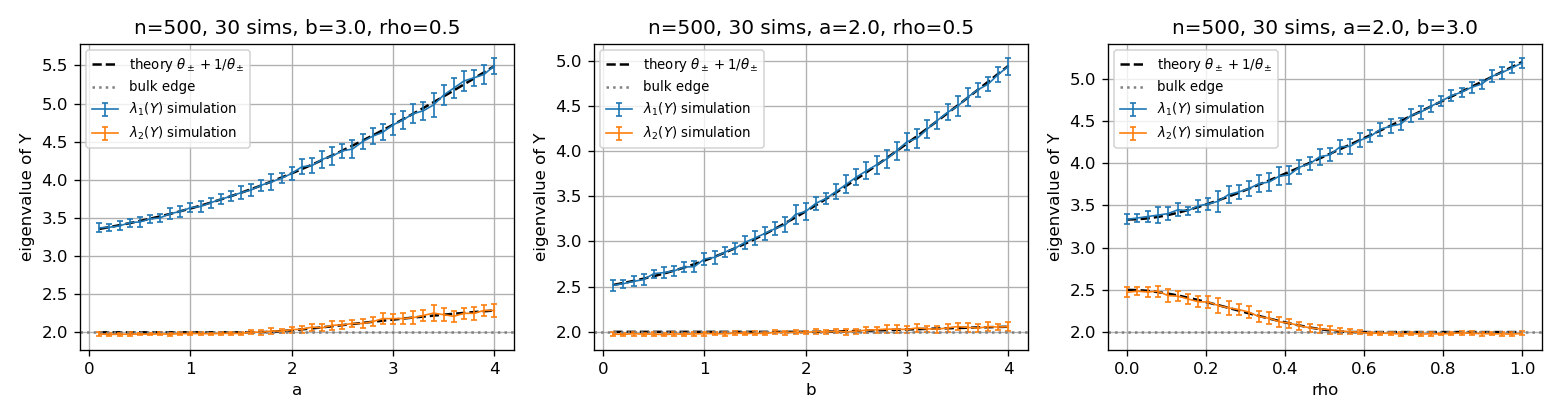
\includegraphics[width=\linewidth]{figures/eigenvalues_Y.png}
    \caption{eigenvalues Y}
    \label{fig:eigenvalues_Y}
\end{figure}




\begin{figure}[ht] 
    \centering 
    \hspace*{-1.3cm}
   \begin{subfigure}{0.3\textwidth}
        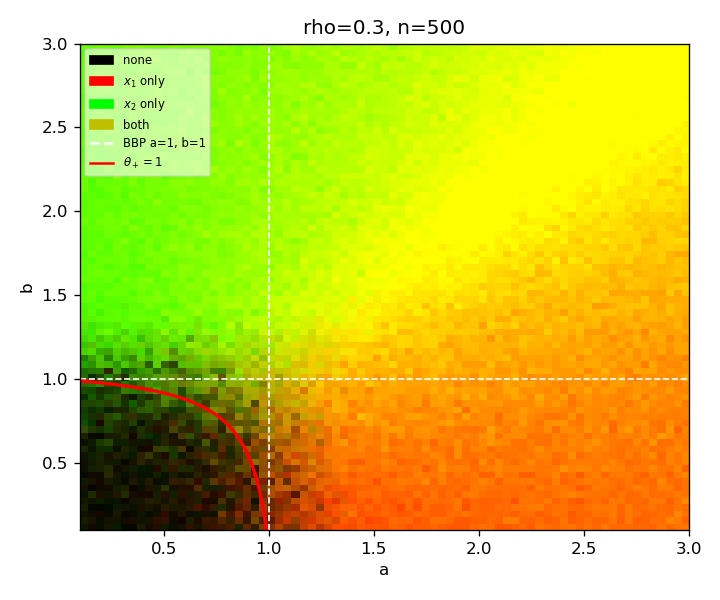
\includegraphics[width=\textwidth]{figures/phase_rho=0.3.png}
                \caption{}

    \end{subfigure}
    \begin{subfigure}{0.7\textwidth}
    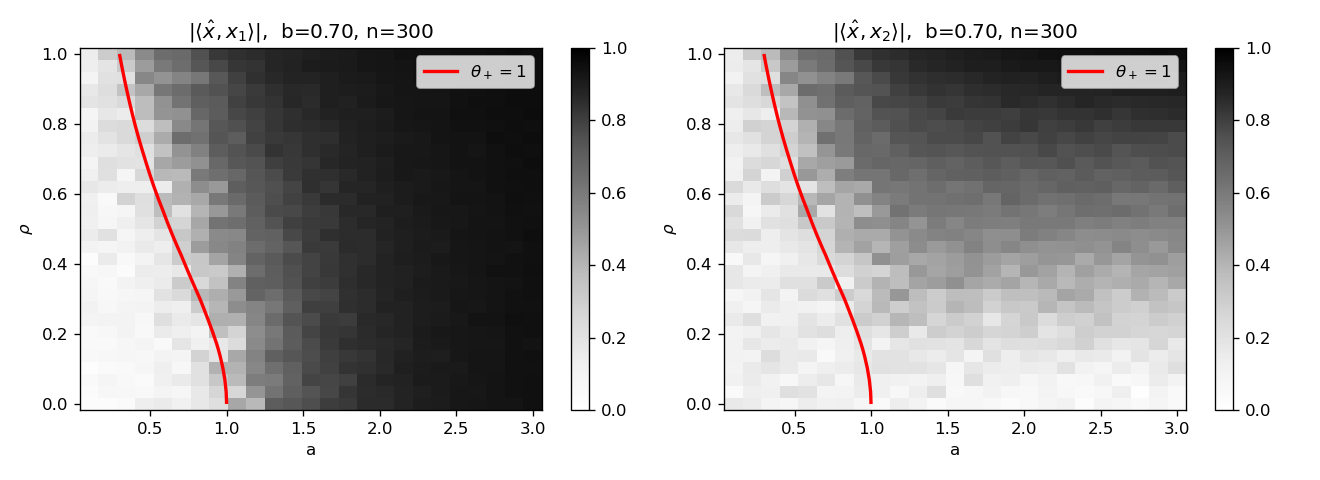
\includegraphics[width=\textwidth]{figures/heat_a_rho.png}
            \caption{}

    \end{subfigure}
  \caption{Recovery thershold}
  \label{fig:overlap_naive}
\end{figure}

\begin{figure}[H]
    \centering
    \includegraphics[width=0.4\linewidth]{figures/overlaps_vs_lambda.png}
    \caption{}
    \label{fig:placeholder}
\end{figure}



\begin{comment}


\section{First Step}

IDEE DE PLAN/TRAJECTOIRE (à partir de la section 6 pour avoir la vision):
\begin{itemize}
    \item 1- \textbf{Comment on a crée/ quelles sont nos méthode EWC :} On pose notre Loss EWC (inspiré du paper) -> methodes découlant de cette loss: méthode A et B (bien appuyer sur sequentialité step 1 puis step 2) 
    
    \item 2- \textbf{Step 1:} overlap $m_1$, transition $\lambda_1 >1$, formulation théorique de notre estimateur (garder uniquement $\hat x^{(1)}_{P_1}$ les autres en annexe peut etre)
    
    \item 3- \textbf{En préparation du Step 2:} Etude de la matrice Hessienne A évalué en $\hat x^{(1)}_{P_1}$: 
    
    Eigenvalues, transition, overlaps avec signaux
    
    (motivation: elle est centrale dans nos deux méthodes étant donné que c'est la Hessienne de notre Loss)
    \textit{Ici on ne parle pas encore d'estimateur du step 2, uniquement d'eigenvalue et eigenvector}

    \item 4- \textbf{Methode A:}
    Estimateur final au Step 2: 
    
    top(A), condition pour retrouver le signal ($\theta_{max}>1$), overlapp avec les deux signaux

    \item 5- \textbf{Methdode B:}
    Estimateur final: ecrire l'expression dans la base de A, condition pour retrouver le signal ($\theta_{max}>1$ au moins 1 spike qui sort du bulk -> au moins un overlap non nul), overlapp avec les deux signaux

\end{itemize}

Recover the first signal $\vect{x_1}$ Let us define our fist-step estimator $\hat{\vect x}^{(1)}$ as the top eigenvector of the first observaation $\rdmmat Y_1 = \lambda_1 \vect x_1 \vect x_1 ^T + \rdmmat Z_1$ 
\subsection{Ideal case: complete recovery}
We consider that in the first step our estimator of the signal completely recovers it.
For the approximation of a perfect recovery of the first signal ($ \hat{\vect x}^{(1)} = \vect x_1$), the Hessian is of the form $\rdmmat A = \rdmmat P + \rdmmat W + c \rdmmat I_n$ where:
\[
\begin{cases}
    \rdmmat P = a \vect x_1 \vect x_1^T + b \vect x_2 \vect x_2^T \qquad \text{with} \quad a = 2\mu_R \Big((\lambda_1-1)^2 + \frac{1}{n} \Big) > 0, \quad b = \lambda_2 \\
    \rdmmat W = \rdmmat Z _2\\
    c = \Big(\frac{2\mu_R}{n} - 1 \Big) 
\end{cases}
\]
The recovery transitions are then given by the general results of section \ref{sec:general_results}.

\subsection{Non-Ideal case: partial recovery}
We consider a way to approximate the first step estimator $\hat{\vect x}^{(1)}$.

\subsubsection{Estimation via first time step overlap}
The first time step overlap with the signal $m_1$, represents the recovered fraction of the signal $\vect x_1$. An possible approximation of our estimator is then:

\begin{equation}
\boxed{\;
    \hat{\vect x}^{(1)}_{m_1} = m_1 \vect x_1\;
    }
    \label{eq:x_hat_m1}
\end{equation}
Then as for the perfect recovery, the Hessian is of the form $\rdmmat A = \rdmmat P + \rdmmat W + c \rdmmat I_n$.
The recovery transitions are then given by Eq. \ref{eq:BBP_overlap_k_spikes} and Eq. \ref{eq:BBP-k-spikes}, with $k=2$ and the parameters:
\[
\begin{cases}
     a = 2\mu_R \Big((\lambda_1-1)^2 + \frac{1}{n} \Big) m_1^2  \\
     b = \lambda_2 \\
    c = \Big(\frac{2\mu_R}{n} - 1 \Big) 
\end{cases}
\]

\subsubsection{Estimation with an orthogonal projector of the signal}
A more complete way to approximate our estimator is to also consider the not recovered part of our signal. Considering a rank one spike $\vect g \in \R^n$ with $g_i \sim \mathcal{N}( 0, 1)$, project on the orthogonal subspace of the signal $\vect x_1$, the estimator can be approximate by:
\begin{equation}
\boxed{
    \hat{\; \vect x}^{(1)}_{P_1} = m_1 \vect x_1 + \sqrt{1 - m_1 ^2} \frac{\rdmmat P_{\perp x_1}\vect g}{\norm{P_{\perp x_1}\vect g}} \;} \quad \text{with} \quad \rdmmat P_{\perp x_1} = \rdmmat I - \vect x_1 \vect x_1^\top
    \label{eq:x_hat_p1}
\end{equation}
defining a rotated spike $\vect x_3 = \frac{\rdmmat P_{\perp x_1}\vect g}{\norm{P_{\perp x_1}\vect g}} $, the Hessian matrix $\rdmmat A$ is given, as before, by $ \rdmmat A = \rdmmat P + \rdmmat W + c \rdmmat I_n$ with:
\[
\rdmmat P = \alpha_{11} \vect x_1 \vect x_1^T + \alpha_{22} \vect x_2 \vect x_2^T + \alpha_{33} \vect x_3 \vect x_3^T + \alpha_{13}\big( \vect x_1 \vect x_3^T + \vect x_3 \vect x_1^T \big)
\]
and the coefficients:
\[
\begin{cases}
     \alpha_{11} = 2\mu_R \Big((\lambda_1-1)^2 + \frac{1}{n} \Big) m_1^2  \\
     \alpha_{22} = \lambda_2 \\
     \alpha_{33} = 2\mu_R \Big((\lambda_1-1)^2 + \frac{1}{n} \Big)(1 -m_1^2) \\
     \alpha_{13} = 2\mu_R \Big((\lambda_1-1)^2 + \frac{1}{n} \Big) m_1 \sqrt{1- m_1^2}
\end{cases}
\]
The orthonormal basis of $(\vect e_1, \vect e_2, \vect e_3)$ of $\rdmmat P$ is:
\[
\begin{cases}
    \vect x_1 = \vect e_1 \\
    \vect x_2 = \rho \vect e_1 + \Tilde{\rho} \vect e_3 + \sqrt{1 - \rho^2 - \Tilde{\rho}^2} \vect e_2 \\
    \vect x_3 = \vect e_3
\end{cases}
\]
Where $\rho$ is the imposed correlation between signal 1 and signal 2 ($\lvert \langle \vect x_1, \vect x_2 \rangle \rvert \xrightarrow[n\to\infty]{\text{a.s.}} \rho $) and $\Tilde{\rho}$ is the induced correlation between the second signal and our created third spike ($\lvert \langle \vect x_2, \vect x_3 \rangle \rvert = \Tilde{\rho} \rangle \rvert \approx \frac{1}{\sqrt n} \xrightarrow[n\to\infty]{\text{a.s.}} 0$).
In this basis, the matrix $\rdmmat P$ is then:
\begin{comment}
\[
\begin{aligned}
\rdmmat{P} = &{}
(\alpha_{11}+\alpha_{22}\rho^2)\,
\vect e_1 \vect e_1^T
+\alpha_{22}(1-\rho^2-\widetilde{\rho}^{\,2})\,
\vect e_2 \vect e_2^T
 +(\alpha_{33}+\alpha_{22}\widetilde{\rho}^{\,2})\,
\vect e_3 \vect e_3^T
\\
&+\alpha_{22}\rho\sqrt{1-\rho^2-\widetilde{\rho}^{\,2}}\,
\left(\vect e_1 \vect e_2^T+\vect e_2 \vect e_1^T\right)
+(\alpha_{13}+\alpha_{22}\rho\widetilde{\rho})\,
\left(\vect e_1 \vect e_3^T+\vect e_3 \vect e_1^T\right)
+\alpha_{22}\widetilde{\rho}\sqrt{1-\rho^2-\widetilde{\rho}^{\,2}}\,
\left(\vect e_2 \vect e_3^T+\vect e_3 \vect e_2^T\right). 
\end{aligned}
\]
Leading to:

\[ 
\rdmmat P =  \sum_{i,j = 1}^3 \beta_{ij} \vect e_i \vect e_j^T
\]
where the coefficients $\beta_{ij} \equiv \beta_{ij}(\lambda_1, m_1, \lambda_2, \mu_R,\rho, \Tilde{\rho})$ are given in the annex table \ref{tab:coefficients_beta_A(xP1)}.
\paragraph{Remark} As the third spike $\vect x_3$ has no preferred direction except it's orthogonality with $\vect x_1$, for $n$ large enough, it's overlap with the second signal $\vect x_2$ tend to zero.
\[
    \Tilde{\rho}= \lvert \langle \vect x_2, \vect x_3 \rangle \rvert \approx \frac{1}{\sqrt n} \xrightarrow[n\to\infty]{\text{a.s.}} 0
\]
In the limit $\widetilde{\rho}\to 0$, the matrix
Let \(\rdmmat B\) be the real symmetric matrix
\[
\rdmmat B=
\begin{pmatrix}
\beta_{11}&\beta_{12}&\beta_{13}\\
\beta_{12}&\beta_{22}& 0\\
\beta_{13}& 0 &\beta_{33}
\end{pmatrix}.
\]
has entries detailed in T\ref{truc}. And it's top eigenvalue is:

\[
\begin{aligned}
\beta_{11}&=\alpha_{11}+\alpha_{22}\rho^2, &
\beta_{22}&=\alpha_{22}(1-\rho^2), &
\beta_{33}&=\alpha_{33},\\
\beta_{12}&=\alpha_{22}\,\rho\sqrt{1-\rho^2}, &
\beta_{13}&=\alpha_{13}, &
\beta_{23}&=0 .
\end{aligned}
\]
Its eigenvalues are denoted $\theta_1\geq\theta_2\geq\theta_3$.

\paragraph{Top eigenvalue.}
Let
\[
T=\beta_{11}+\beta_{22}+\beta_{33},\qquad
Q=\beta_{11}\beta_{22}+\beta_{11}\beta_{33}+\beta_{22}\beta_{33}
-\beta_{12}^2-\beta_{13}^2,
\]
\[
D=\beta_{11}\beta_{22}\beta_{33}-\beta_{22}\beta_{13}^2-\beta_{33}\beta_{12}^2,
\qquad \Delta=T^2-3Q>0 .
\]
\[
\boxed{
\theta_1=\frac{T}{3}+\frac{2\sqrt{\Delta}}{3}
\cos\!\left(\frac13\arccos\!\left(\frac{2T^3-9TQ+27D}{2\Delta^{3/2}}\right)\right).
}
\]
Details of the computation in \ref{true}.

    
\end{comment}


\subsection{Spectrum of the Hessian $\rdmmat A$}\label{sec:hessian_A}
\subsubsection{First-step estimator}
The first-step estimator $\hat{\vect x}^{(1)}$ is the top eigenvector of $\rdmmat Y_1 = \lambda_1 \vect x_1 \vect x_1 ^T + \rdmmat Z_1$. By Theorem~\ref{thm:bbp}, its overlap with $\vect x_1$ converges to
\begin{equation}
    m_1 := \begin{cases}
        0 & \text{if } \lambda_1 \le 1,\\[0.3em]
        \sqrt{1-\lambda_1^{-2}} & \text{if } \lambda_1 > 1.
    \end{cases}
    \label{eq:lambda_max_Y1}
\end{equation}
To study the second step analytically, we replace $\hat{\vect x}^{(1)}$ by the unit vector with the same overlap,
\begin{equation}
    \hat{\vect x}^{(1)}_{P_1} = m_1\vect x_1 + \sqrt{1-m_1^2}\,\vect x_3 ,
    \label{eq:x_hat_p1}
\end{equation}
where $\vect x_3$ is a unit vector orthogonal to $\vect x_1$, independent of $\rdmmat Z_2$.

\subsubsection{The matrix}
We evaluate the Hessian at the projector estimator $\hat{\vect x}^{(1)}_{P_1}$ of Eq.~\eqref{eq:x_hat_p1}. Since $\norm{\hat{\vect x}^{(1)}_{P_1}} = 1$, the Fisher matrix of Appendix~\ref{adix:fisher} gives
\begin{equation}
    \rdmmat A = \rdmmat Y_2 - \rdmmat I_n + 2\mu_R\,\rdmmat F\big(\hat{\vect x}^{(1)}_{P_1}\big)
    = \underbrace{\Lambda\,\hat{\vect x}^{(1)}_{P_1}\hat{\vect x}^{(1)\top}_{P_1} + \lambda_2\,\vect x_2\vect x_2^\top}_{\rdmmat P}
    + \underbrace{\rdmmat Z_2}_{\rdmmat W} + c\,\rdmmat I_n,
    \qquad
    \Lambda = 2\mu_R\Big((\lambda_1-1)^2 + \frac1n\Big), \quad c = \frac{2\mu_R}{n} - 1 .
    \label{eq:A_xP1}
\end{equation}
This is the form $\rdmmat A = \rdmmat P + \rdmmat W + c\,\rdmmat I_n$ of Section~\ref{sec:model}, with $k=3$: in the orthonormal basis $\vect e_1 = \vect x_1$, $\vect e_2$, $\vect e_3 = \vect x_3$, $\rdmmat P = \rdmmat E \rdmmat B \rdmmat E^T$ with the coefficients of Table~\ref{tab:beta_A} in Appendix~\ref{tab:coefficients_beta_A(xP1)}. Its explicit form in the large $n$ limit is given in Eq.~\eqref{eq:B_A_limit}.

\subsubsection{Eigenvalues and eigenvectors}
\begin{prop}[Spectrum of $\rdmmat A$]\label{prop:spectrum_A}
Let $m_1\rho > 0$. The eigenvalues $\theta_1\ge\theta_2\ge\theta_3$ of $\rdmmat B$ are
\begin{equation}
    \theta_{1,2} = \frac{\Lambda+\lambda_2}{2} \pm \sqrt{\Big(\frac{\Lambda-\lambda_2}{2}\Big)^2 + \Lambda\lambda_2\,m_1^2\rho^2},
    \qquad \theta_3 = 0 ,
    \label{eq:theta_A}
\end{equation}
and, almost surely as $n\to\infty$, the three largest eigenvalues of $\rdmmat A$ converge to
\begin{equation}
    \lambda^{\mathrm{out}}_l \longrightarrow
    \begin{cases}
        \theta_l + \dfrac{1}{\theta_l} + c, & \theta_l > 1,\\[6pt]
        2 + c, & \theta_l \le 1,
    \end{cases}
    \quad l = 1,2,
    \qquad\qquad
    \lambda^{\mathrm{out}}_3 \longrightarrow 2 + c .
    \label{eq:outliers_A}
\end{equation}
For $l=1,2$, the eigenvectors of $\rdmmat P$ associated with $\theta_l$ and their overlaps $q_i^l = \langle\vect v_l,\vect x_i\rangle$ with the spikes are
\begin{equation}
    \vect v_l = c_1^l\,\hat{\vect x}^{(1)}_{P_1} + c_2^l\,\vect x_2, \qquad
    \big(c_1^l, c_2^l\big) = \frac{(r_l,\,1)}{\sqrt{r_l^2 + 2m_1\rho\,r_l + 1}}, \qquad
    r_l = \frac{m_1\rho\,\Lambda}{\theta_l - \Lambda} ,
    \label{eq:v_A} 
\end{equation}
\begin{equation}
    q_1^l = m_1\,c_1^l + \rho\,c_2^l, \qquad
    q_2^l = \frac{\theta_l}{\lambda_2}\,c_2^l, \qquad
    q_3^l = \sqrt{1-m_1^2}\;c_1^l ,
    \label{eq:q_A}
\end{equation}
and the unit eigenvectors $\vect u_1,\vect u_2,\vect u_3$ of $\rdmmat A$ associated with its three largest eigenvalues satisfy, for $i=1,2,3$,
\begin{equation}
    |\langle\vect u_l,\vect x_i\rangle| \longrightarrow
    \begin{cases}
        |q_i^l|\sqrt{1-\theta_l^{-2}}, & \theta_l > 1,\\
        0, & \theta_l \le 1,
    \end{cases}
    \quad l=1,2,
    \qquad
    |\langle\vect u_3,\vect x_i\rangle| \longrightarrow 0 .
    \label{eq:overlaps_A}
\end{equation}
\end{prop}
\begin{proof}
$\rdmmat P$ is built from the two vectors $\hat{\vect x}^{(1)}_{P_1}$ and $\vect x_2$, so it has rank $2$ and $\theta_3 = 0$. It has the structure of the naive signal matrix of Eq.~\eqref{eq:2spikes} with $a\to\Lambda$, $b\to\lambda_2$ and $\rho\to m_1\rho = \langle\hat{\vect x}^{(1)}_{P_1},\vect x_2\rangle$, which gives Eq.~\eqref{eq:theta_A} and, by the derivation of Appendix~\ref{sec:eigenvect_naive}, Eq.~\eqref{eq:v_A}. Eq.~\eqref{eq:q_A} follows from $\langle\vect x_1,\vect x_2\rangle = \rho$, $\langle\vect x_1,\vect x_3\rangle = 0$, $\langle\vect x_2,\vect x_3\rangle\to0$ and Eq.~\eqref{eq:overlaps-signals}. Eqs.~\eqref{eq:outliers_A} and~\eqref{eq:overlaps_A} are Theorem~\ref{thm:bbp_k} and Corollary~\ref{cor:overlap_signals}.
\end{proof}
\noindent
Since $\theta_3 = 0$, the third eigenvector belongs to the bulk and carries no information on the spikes: $\rdmmat A$ has at most two outliers. The eigenvectors and the overlaps do not depend on $c$, which only shifts the eigenvalues.

\subsubsection{Transitions}\label{sec:transitions_A}
By Eq.~\eqref{eq:outliers_A}, the number of outliers of $\rdmmat A$ is the number of $\theta_l > 1$. By Eq.~\eqref{eq:theta_A}, $\theta_1$ and $\theta_2$ are the roots of
\begin{equation}
    p(\theta) = \theta^2 - (\Lambda + \lambda_2)\,\theta + \Lambda\lambda_2(1 - m_1^2\rho^2) ,
    \label{eq:p_theta}
\end{equation}
where $\Lambda$ and $m_1 = \sqrt{1-\lambda_1^{-2}}$ (or $0$ for $\lambda_1 \le 1$) depend on $\lambda_1$ only. Solving $p(1)=0$ for $\lambda_2$ defines the two boundaries
\begin{equation}
    f_{01}(\lambda_1) = \frac{1-\Lambda}{1-\Lambda(1-m_1^2\rho^2)} \quad \text{for } \Lambda < 1,
    \qquad
    f_{12}(\lambda_1) = \frac{\Lambda-1}{\Lambda(1-m_1^2\rho^2)-1} \quad \text{for } \Lambda(1-m_1^2\rho^2) > 1 ,
    \label{eq:f01_f12}
\end{equation}
which are the same function of $\lambda_1$ on two different branches.

\begin{prop}[Phase diagram of $\rdmmat A$]\label{prop:phase_A}
In the $(\lambda_1, \lambda_2)$ plane, almost surely as $n\to\infty$, $\rdmmat A$ has
\begin{itemize}
    \item \textbf{no outlier} if $\Lambda < 1$ and $\lambda_2 < f_{01}(\lambda_1)$;
    \item \textbf{two outliers} if $\Lambda(1-m_1^2\rho^2) > 1$ and $\lambda_2 > f_{12}(\lambda_1)$;
    \item \textbf{one outlier} otherwise.
\end{itemize}
\end{prop}
\noindent
The proof is given in Appendix~\ref{adix:phase_A}. Since $f_{01} \le 1 \le f_{12}$, two outliers require $\lambda_2 > 1$, and $\lambda_2 > 1$ guarantees at least one. Equivalently, solving $p(1) = 0$ for $\Lambda$, the top eigenvalue leaves the bulk ($\theta_1 > 1$) if and only if $\lambda_2 > 1$ or $\Lambda > \Lambda^*$, with
\begin{equation}
    \Lambda^* = \frac{\lambda_2 - 1}{\lambda_2\,(1-m_1^2\rho^2) - 1},
    \qquad
    \mu_R^* = \frac{\Lambda^*}{2\big((\lambda_1-1)^2 + \frac1n\big)} .
    \label{eq:Lambda_star}
\end{equation}

\subsection{Method A: top eigenvector of the Hessian}\label{sec:methodA}
Method A takes as estimator the top eigenvector of $\rdmmat A$:
\begin{equation}
    \hat{\vect x}^{(2)}_{A} = \text{top eigenvector}(\rdmmat A) = \vect u_1 .
    \label{eq:x_hat_a}
\end{equation}
We write $\theta_{max} \equiv \theta_1$ for the largest eigenvalue of $\rdmmat B$, given by Eq.~\eqref{eq:theta_A}.

\begin{prop}[Method A]\label{prop:methodA}
Let $m_1\rho > 0$. Almost surely as $n\to\infty$:
\begin{enumerate}[(i)]
    \item the top eigenvalue of $\rdmmat A$ converges to
    \begin{equation}
        \lambda^{\mathrm{out}}_{max} \longrightarrow
        \begin{cases}
            \theta_{max} + \dfrac{1}{\theta_{max}} + \dfrac{2\mu_R}{n} - 1, & \theta_{max} > 1,\\[6pt]
            1 + \dfrac{2\mu_R}{n}, & \theta_{max} \le 1 ;
        \end{cases}
        \label{eq:top_eigenvalue_A}
    \end{equation}
    \item the estimator carries information on the signals if and only if
    \begin{equation}
        \theta_{max} > 1
        \quad\Longleftrightarrow\quad
        \lambda_2 > 1
        \quad\text{or}\quad
        \mu_R > \mu_R^* ,
        \label{eq:condition_A}
    \end{equation}
    with $\mu_R^*$ of Eq.~\eqref{eq:Lambda_star};
    \item its overlaps with the signals converge to
    \begin{equation}
        m^A_1 := |\langle \hat{\vect x}^{(2)}_A, \vect{x_1}\rangle| \longrightarrow \big\lvert m_1 c_1^1 + \rho\, c_2^1 \big\rvert \sqrt{1-\theta_{max}^{-2}} ,
        \qquad
        m^A_2 := |\langle \hat{\vect x}^{(2)}_A, \vect{x_2}\rangle| \longrightarrow \Big \lvert  \frac{\theta_{max}}{\lambda_2}c_2^1  \Big \rvert \sqrt{1-\theta_{max}^{-2}}
        \label{eq:overlap_A}
    \end{equation}
    for $\theta_{max} > 1$, and to $0$ for $\theta_{max} \le 1$, with $c_1^1, c_2^1$ of Eq.~\eqref{eq:v_A}.
\end{enumerate}
\end{prop}
\begin{proof}
(i) and (iii) are Eqs.~\eqref{eq:outliers_A} and~\eqref{eq:overlaps_A} of Proposition~\ref{prop:spectrum_A} with $l=1$, $c = \frac{2\mu_R}{n}-1$ and $q_i^1$ of Eq.~\eqref{eq:q_A}. (ii) is the condition for at least one outlier in Proposition~\ref{prop:phase_A}, written with $\Lambda^*$ of Eq.~\eqref{eq:Lambda_star}.
\end{proof}
\noindent
When the second signal is detectable on its own ($\lambda_2>1$), Method A always recovers information. Otherwise, the EWC penalty has to be strong enough to push $\theta_{max}$ above $1$: the regularisation alone can make the estimator leave the bulk. The overlaps have the same form as those of the naive method, Eq.~\eqref{eq:overlap_naive}, with $a \to \Lambda$, $b \to \lambda_2$ and $\rho \to m_1\rho$. Similarly, $m^A_3 = |\langle \hat{\vect x}^{(2)}_A, \vect{x_3}\rangle| \to \sqrt{1-m_1^2}\,|c_1^1|\sqrt{1-\theta_{max}^{-2}}$ measures the part of the first-step error inherited by the second-step estimator.

\subsection{Method B: resolvent of the Hessian}\label{sec:methodB}
Method B takes as estimator the solution of the stationarity condition with the Lagrange shift, Eq.~\eqref{eq:final_estimator_lagrange}:
\begin{equation}
    \hat{\vect x}^{(2)}_B(\lambda) = 2\mu_R\,\vect R_{\rdmmat A}(\lambda)\,\vect F_1 \hat{\vect x}^{(1)},
    \qquad \norm{\hat{\vect x}^{(2)}_B(\lambda)} = 1 ,
    \label{eq:x_hat_b}
\end{equation}
with $\hat{\vect x}^{(1)} = \hat{\vect x}^{(1)}_{P_1}$. For a unit vector $\vect x$, $\rdmmat F(\vect x)\,\vect x = \big((\lambda_1-1)^2 + \frac2n\big)\vect x$, so
\begin{equation}
    \hat{\vect x}^{(2)}_B(\lambda) = \kappa\,\vect R_{\rdmmat A}(\lambda)\,\hat{\vect x}^{(1)},
    \qquad
    \kappa = 2\mu_R\Big((\lambda_1-1)^2 + \frac2n\Big) ,
    \label{eq:xB_basisA}
\end{equation}
and the multiplier $\lambda$ is selected as the unique root of the norm constraint above the top eigenvalue $\gamma_1$ of $\rdmmat A$ (Appendix~\ref{app:B_resolvent}).

\noindent
The limit is expressed with the Stieltjes transform of the semicircle law (Appendix~\ref{proof:BBP1}), $S_W(z) = \frac{z - \sqrt{z^2-4}}{2}$ for $z>2$, which satisfies $-S_W'(z) = \frac{S_W(z)^2}{1-S_W(z)^2} > 0$, and with the overlaps $q_{il} := q_i^l$ of Eq.~\eqref{eq:q_A} and
\begin{equation}
    q_{sl} := \langle \vect v_l, \hat{\vect x}^{(1)}\rangle = \frac{\theta_l}{\Lambda}\,c^l_1 , \qquad l = 1,2,
\end{equation}
which follows from Eq.~\eqref{eq:overlaps-signals} with $a\to\Lambda$ and $\vect x_1\to\hat{\vect x}^{(1)}$. Since $\theta_3 = 0$ and $\hat{\vect x}^{(1)} \in \mathrm{span}(\vect v_1,\vect v_2)$, $q_{s3} = 0$.

\begin{prop}[Method B]\label{prop:B_overlaps}
Assume $m_1\rho > 0$ and let
$z_* := \max\!\big(2,\ \max_{l:\,\theta_l > 1}(\theta_l + \theta_l^{-1})\big)$, the right edge of the spectrum of $\rdmmat A - c\rdmmat I_n$.
Then, almost surely as $n\to\infty$, the selected multiplier converges, $\lambda \to c + z^\star$,
where $z^\star$ is the unique solution on $(z_*,\infty)$ of
\begin{equation}
    \kappa^2 \sum_{l=1}^{2} q_{sl}^2\,
    \frac{-S_W'(z)}{\big(1-\theta_l S_W(z)\big)^2} = 1 ,
    \label{eq:B_norm}
\end{equation}
and the overlaps of the estimator with the signals converge to
\begin{equation}
    m^B_i := \big|\langle \hat{\vect x}^{(2)}_B, \vect x_i\rangle\big|
    \longrightarrow
    \kappa\, \left| \sum_{l=1}^{2} q_{il}\, q_{sl}\,
    \frac{S_W(z^\star)}{1-\theta_l S_W(z^\star)} \right| ,
    \qquad i = 1,2,3 .
    \label{eq:B_overlap}
\end{equation}
\end{prop}
\noindent
The proof is given in Appendix~\ref{app:B_resolvent}. The resolvent of Eq.~\eqref{eq:xB_basisA} involves all $n$ eigenvectors of $\rdmmat A$, but its projection on the signal subspace reduces to a $2\times 2$ problem: the bulk eigenvectors are individually random, but their total contribution is captured by $S_W$. Near an outlier, $z \to \theta_l + \theta_l^{-1}$, one has $S_W(z) \to 1/\theta_l$ and
\[
    \frac{S_W(z)}{1-\theta_l S_W(z)} \simeq \frac{1-\theta_l^{-2}}{\theta_l + \theta_l^{-1} + c - \lambda} ,
\]
so the pole part of Eq.~\eqref{eq:B_overlap} is the contribution of the outlier eigenvector $\vect u_l$ given by Corollary~\ref{cor:overlap_signals}, and the regular remainder is the contribution of the bulk.

\noindent
\textbf{No sharp transition.} Unlike Method A, Method B has no recovery threshold. The left-hand side of Eq.~\eqref{eq:B_norm} diverges as $z \to z_*^+$ (through the pole $1-\theta_{\max}S_W = 0$ if $\theta_{\max} > 1$, through $-S_W' \to \infty$ as $z\to 2^+$ otherwise) and vanishes as $z\to\infty$, so a root always exists. Even for $\theta_{\max} \le 1$, Eq.~\eqref{eq:B_overlap} is non-zero as soon as $q_{il} q_{sl} \neq 0$: the estimator is then built from the bulk eigenvectors only, weighted by their overlap with $\hat{\vect x}^{(1)}$, and keeps information on $\vect x_1$, and on $\vect x_2$ through the correlation $\rho$.




\section{Fixing Regularization and Evaluation of the model}

The model aims to perform well on all the tasks it has learned. To evaluate an estimator $\hat{x}$, we compare
its rank-one reconstruction $\hat{x}\hat{x}^T$ with the observations of each task.

\subsection{Evaluation Loss}\label{sec:eval}

\paragraph{Biased Evaluation Loss}
For given observations $Y_l = \lambda_l x_l x_l^T + Z_l \in \mathbb{R}^{n\times n}$, $l = 1,\dots,k$, and an
estimator $\hat{x} \in \mathbb{R}^n$ built from them, we define the Evaluation Loss as
\begin{equation}
  \mathcal{L}_{biased}(\hat{x}) := \sum_{l=1}^{k} \big\| Y_l - \hat{x}\hat{x}^T \big\|_F^2 .
  \label{eq:train_loss_def}
\end{equation}

Expanding the Frobenius norm, using $\|x_l\| = \|\hat{x}\| = 1$ and $x_l^T Z_l x_l \to 0$, the loss becomes in
the large $n$ limit
\begin{equation}
  \mathcal{L}_{biased}(\hat{x}) = \sum_{l=1}^{k} \Big[ -2\lambda_l\, m_l^2 \;-\; 2\,\varepsilon_l \Big] + \mathrm{cst},
  \qquad
  m_l := |\langle \hat{x}, x_l \rangle|, \quad
  \varepsilon_l := \hat{x}^T Z_l \hat{x}.
  \label{eq:train_loss}
\end{equation}
The full calculation is given in Appendix~\ref{an:exp-loss}.

\paragraph{The signal term.} The first term rewards the alignment of the estimator with each signal, weighted
by the strength $\lambda_l$ of that signal. This is the quantity we actually want to optimize.

\paragraph{The noise term and overfitting.} The second term shows that the loss decreases when the estimator is aligned with the noise $Z_l$. If $\hat{x}$ were
independent of $Z_l$, it would be delocalised on the eigenvectors of $Z_l$ and
$\varepsilon_l \to  0$. 

In other words, $\mathcal{L}_{biased}$ measures how well $\hat{x}\hat{x}^T$ reconstructs the
\emph{observations} (signal and noise), not the \emph{signals}. The estimator overfit the observation by fitting the noise. 

Minimizing
$\mathcal{L}_{\mathrm{eval-biased}}$ would therefore partly favour configurations in which the estimator fits the
noise, which is opposite to our goal of recovering $x_1, \dots, x_k$. 

\paragraph{Unbiased Evaluation Loss}
Let $Y'_l = \lambda_l x_l x_l^T + Z'_l$, $l = 1, \dots, k$, be new observations of the same signals, where
the $Z'_l$ are GOE matrices independent of the $Z_l$, and hence of $\hat{x}$. The test Evaluation Loss is
\begin{equation}
  \mathcal{L}_{\mathrm{eval}}(\hat{x}) := \sum_{l=1}^{k} \big\| Y'_l - \hat{x}\hat{x}^T \big\|_F^2 
\end{equation}

Since $\hat{x}$ is independent of $Z'_l$, $\hat{x}^T Z'_l \hat{x} \to 0$ and the noise term disappears:
\begin{equation}
  \boxed{ \; \mathcal{L}_{\mathrm{eval}}(\hat{x}) = -2 \sum_{l=1}^{k} \lambda_l\, m_l^2 + \mathrm{cst}. \; }
    \label{eq:test_loss}
\end{equation}
A good estimator is then one that maximizes its overlaps with the signals, weighted by their strengths. The
difference between both losses,
\begin{equation}
  \mathcal{L}_{biased} - \mathcal{L}_{eval} = 2 \sum_{l=1}^{k} \varepsilon_l \;\geq\; 0,
\end{equation}
 quantifies how much of the apparent performance on the training data
comes from fitting the noise. The full expression of the noise terms $\varepsilon_l$ for naive method and method A are presented in Appendix \ref{an:Naive-Loss} and \ref{an:A_full_Loss}.




\subsection{Fixing the hyperparameters $\alpha$ and $\mu_R$}
\label{sec:optimal_param}

Each method has    hyperparameter that sets the balance between the two tasks: the importance factor $\alpha$ for the naive method, and the regularisation strength $\mu_R$ for Methods A and B. We fix it such that the estimator learns both tasks as well as possible, i.e.\ such that it minimises the test Evaluation Loss of Eq.~\eqref{eq:test_loss}. Writing $t \in \{\alpha, \mu_R\}$ for the hyperparameter of the method under study, the only terms of $\mathcal L_{\mathrm{eval}}$ that depend on $t$ are the overlaps $m_l(t)$ of the estimator with the signals, so that
\begin{equation}
    t^* = \operatorname*{arg\,min}_{t}\ \mathcal L_{\mathrm{eval}}(t)
    = \operatorname*{arg\,max}_{t}\ \sum_{l=1}^{k}\lambda_l\, m_l(t)^2 .
    \label{eq:t_opt}
\end{equation}
When the optimum lies inside the admissible range ($0 < \alpha^* < 1$ or $0 < \mu_R^* < \infty$), it satisfies the stationarity condition
\begin{equation}
    \frac{\partial\mathcal L_{\mathrm{eval}}}{\partial t}(t^*)
    = -2\sum_{l=1}^{k}\lambda_l\,\frac{\partial\, m_l^2}{\partial t}(t^*) = 0 .
    \label{eq:mu_opt}
\end{equation}
The optimum may also lie at a boundary, for instance $\alpha^* \in \{0, 1\}$ when the two tasks are weakly correlated and mixing them dilutes the signal below the detection threshold. In that case, Eq.~\eqref{eq:mu_opt} does not hold, and Eq.~\eqref{eq:t_opt} must be used directly. The overlaps are given in closed form by Eq.~\eqref{eq:overlap_naive} for the naive method, by Eq.~\eqref{eq:overlap_A} for Method A, and by Eqs.~\eqref{eq:B_norm}--\eqref{eq:B_overlap} for Method B. Equation~\eqref{eq:mu_opt} is therefore a scalar equation, which we solve numerically.

\paragraph{Numerical results.} Figure~\ref{fig:loss_opt} shows the Evaluation Losses of the three methods as functions of their hyperparameter, for $\lambda_1 = 3$, $\lambda_2 = 2$ and $\rho = 0.5$. We draw four observations from it.
\begin{itemize}
    \item \textbf{Theory and simulations agree.} The theoretical test loss $-2\sum_l\lambda_l m_l^2$ matches both the overlaps measured in simulations and the loss evaluated on fresh observations $\rdmmat Y'_l$ with independent noise. The theoretical biased loss of Appendix~\ref{an:Naive-Loss} (naive method) and Appendix~\ref{an:A_full_Loss} (Method A) matches its simulated counterpart. The biased loss of Method B is only shown numerically.

    \item \textbf{The biased loss is optimistic and shifts the optimum.} The biased loss lies about $2$ below the test loss for all three methods. This gap is the generalisation gap $2\sum_l\varepsilon_l$ of Section~\ref{sec:eval}: part of the apparent performance on the training data comes from fitting the noise. The gap is not constant, so it also moves the optimum. Minimising the biased loss would give $\alpha^* \simeq 0.71$ instead of $0.81$, $\mu_R^* \simeq 0.42$ instead of $0.48$ for Method A, and $\mu_R^* \simeq 0.18$ instead of $0.23$ for Method B, i.e.\ systematically less weight on the first task.

    \item \textbf{The optimum is a non-trivial trade-off.} For $\alpha \to 0$ or $\mu_R \to 0$, the estimator is the top eigenvector of $\rdmmat Y_2$, with $m_2^2 = 1 - \lambda_2^{-2}$ and $m_1^2 = \rho^2 m_2^2$: the loss tends to $-2\big(\lambda_1\rho^2 + \lambda_2\big)(1-\lambda_2^{-2}) \simeq -4.1$ (catastrophic forgetting). For $\alpha \to 1$ or $\mu_R \to \infty$, the estimator is $\hat{\vect x}^{(1)}$, with $m_1^2 = 1 - \lambda_1^{-2}$ and $m_2^2 = \rho^2 m_1^2$: the loss tends to $-2\big(\lambda_1 + \lambda_2\rho^2\big)(1-\lambda_1^{-2}) \simeq -6.2$ (no learning of task~$2$). At the optimum, the loss reaches about $-6.7$.

    \item \textbf{The sequential methods match the naive method.} At their optimum, Methods A and B reach a test loss of about $-6.70$, slightly below the $-6.65$ of the naive method, although the naive method sees both observations at the same time. A possible explanation is that the sequential methods only keep the rank-one projection of the first task, $\Lambda\,\hat{\vect x}^{(1)}\hat{\vect x}^{(1)\top}$, and thus discard the bulk noise $\rdmmat Z_1$, whereas the naive method keeps the noise of both observations. The values of $\mu_R^*$ for Methods A and B are not directly comparable, since $\mu_R$ weights different penalties in the two methods.
\end{itemize}

\begin{figure}[t]
    \centering
    \begin{subfigure}[t]{0.32\textwidth}
        \centering
        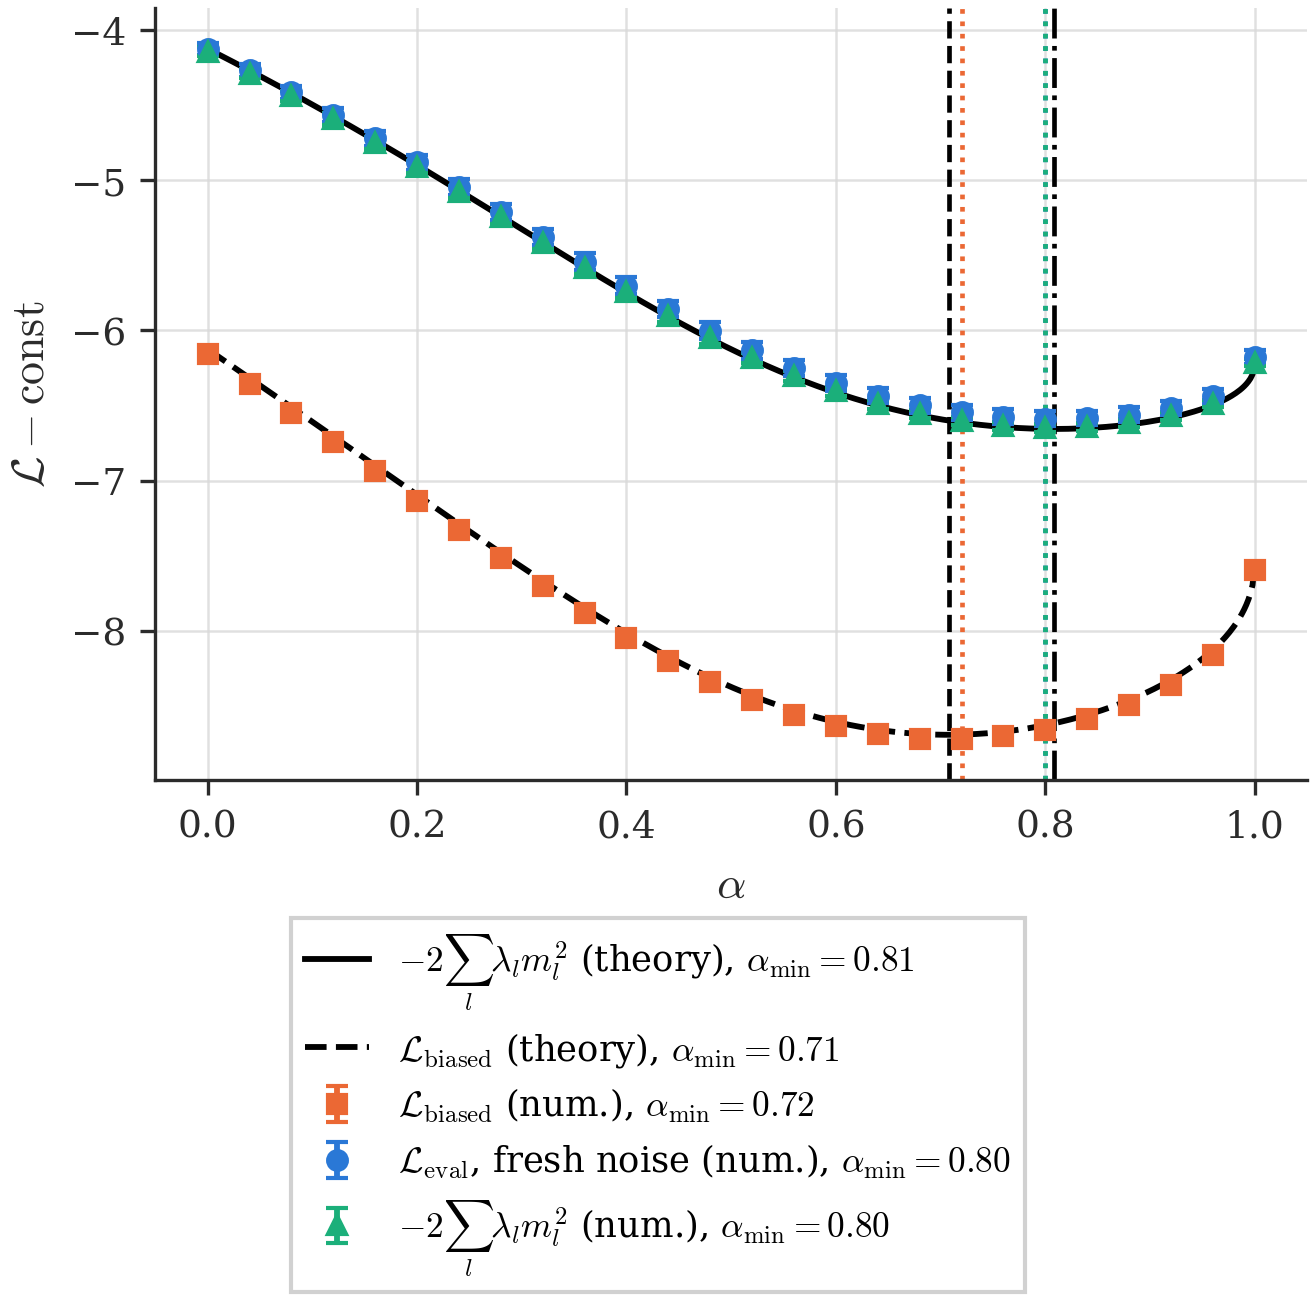
\includegraphics[width=\linewidth]{figures/loss_study/loss_biased_naive_vs_alpha_lam1=3.0_lam2=2.0_rho=0.5_report.png}
        \caption{Naive method, as a function of $\alpha$.}
        \label{fig:loss_opt_naive}
    \end{subfigure}\hfill
    \begin{subfigure}[t]{0.32\textwidth}
        \centering
        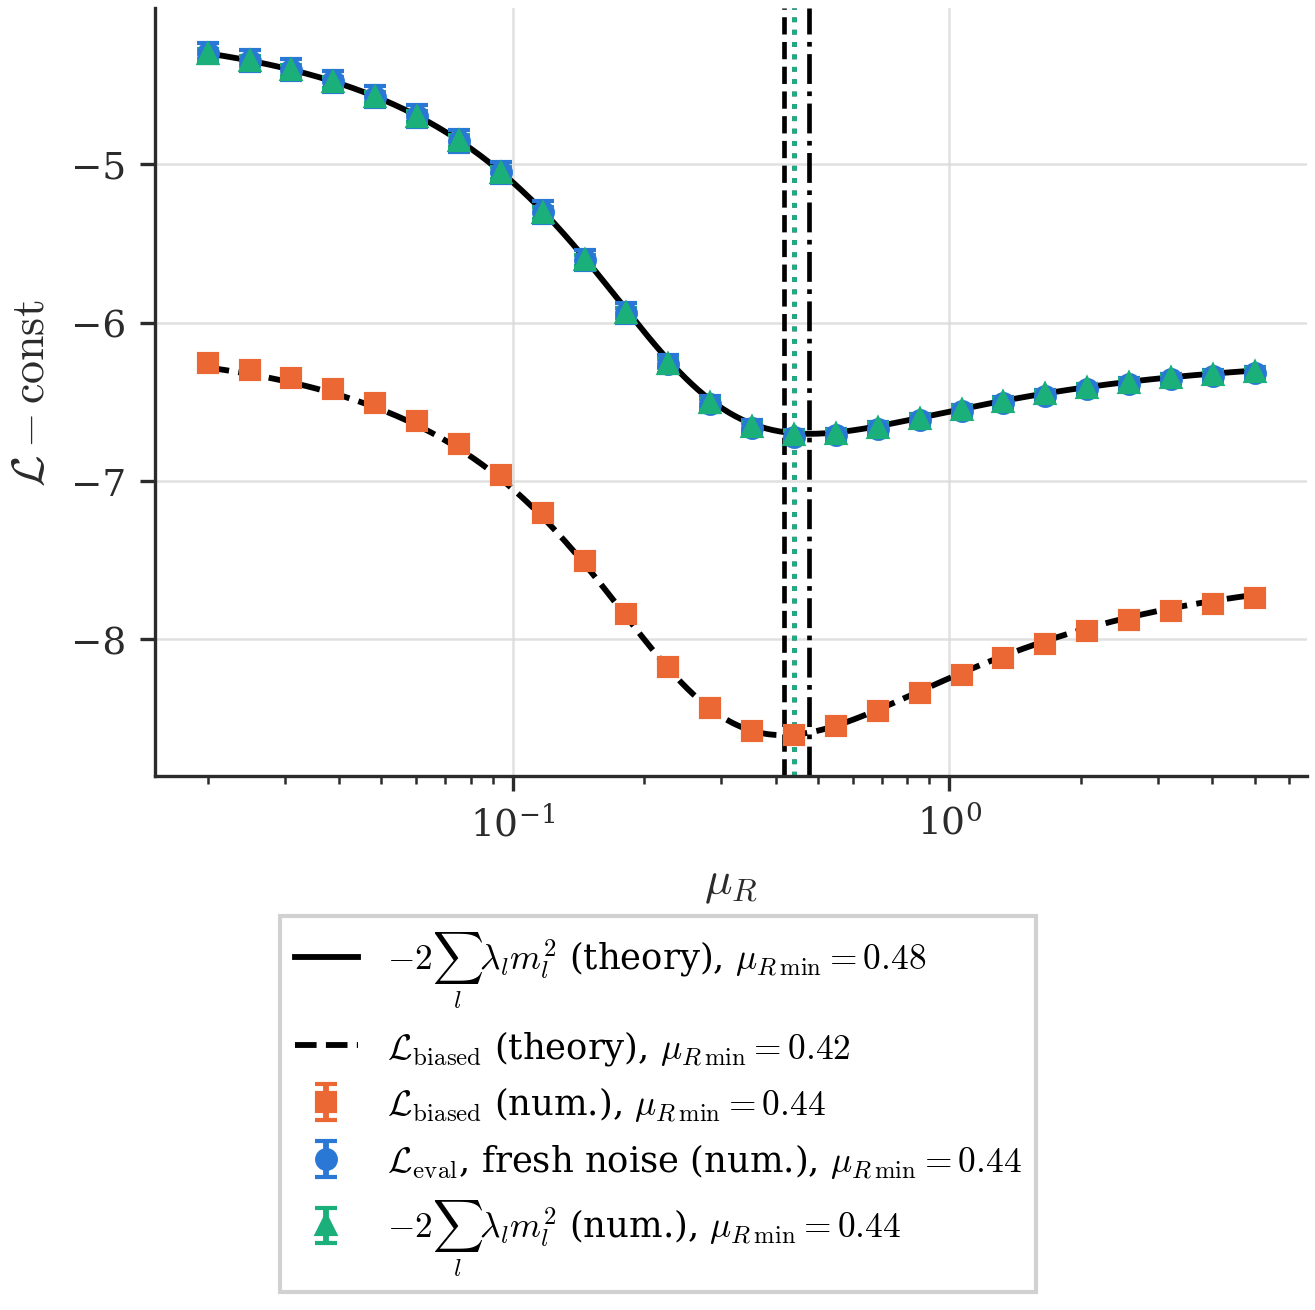
\includegraphics[width=\linewidth]{figures/loss_study/loss_biased_A_vs_mu_lam1=3.0_lam2=2.0_rho=0.5_report.png}
        \caption{Method A, as a function of $\mu_R$.}
        \label{fig:loss_opt_A}
    \end{subfigure}\hfill
    \begin{subfigure}[t]{0.32\textwidth}
        \centering
        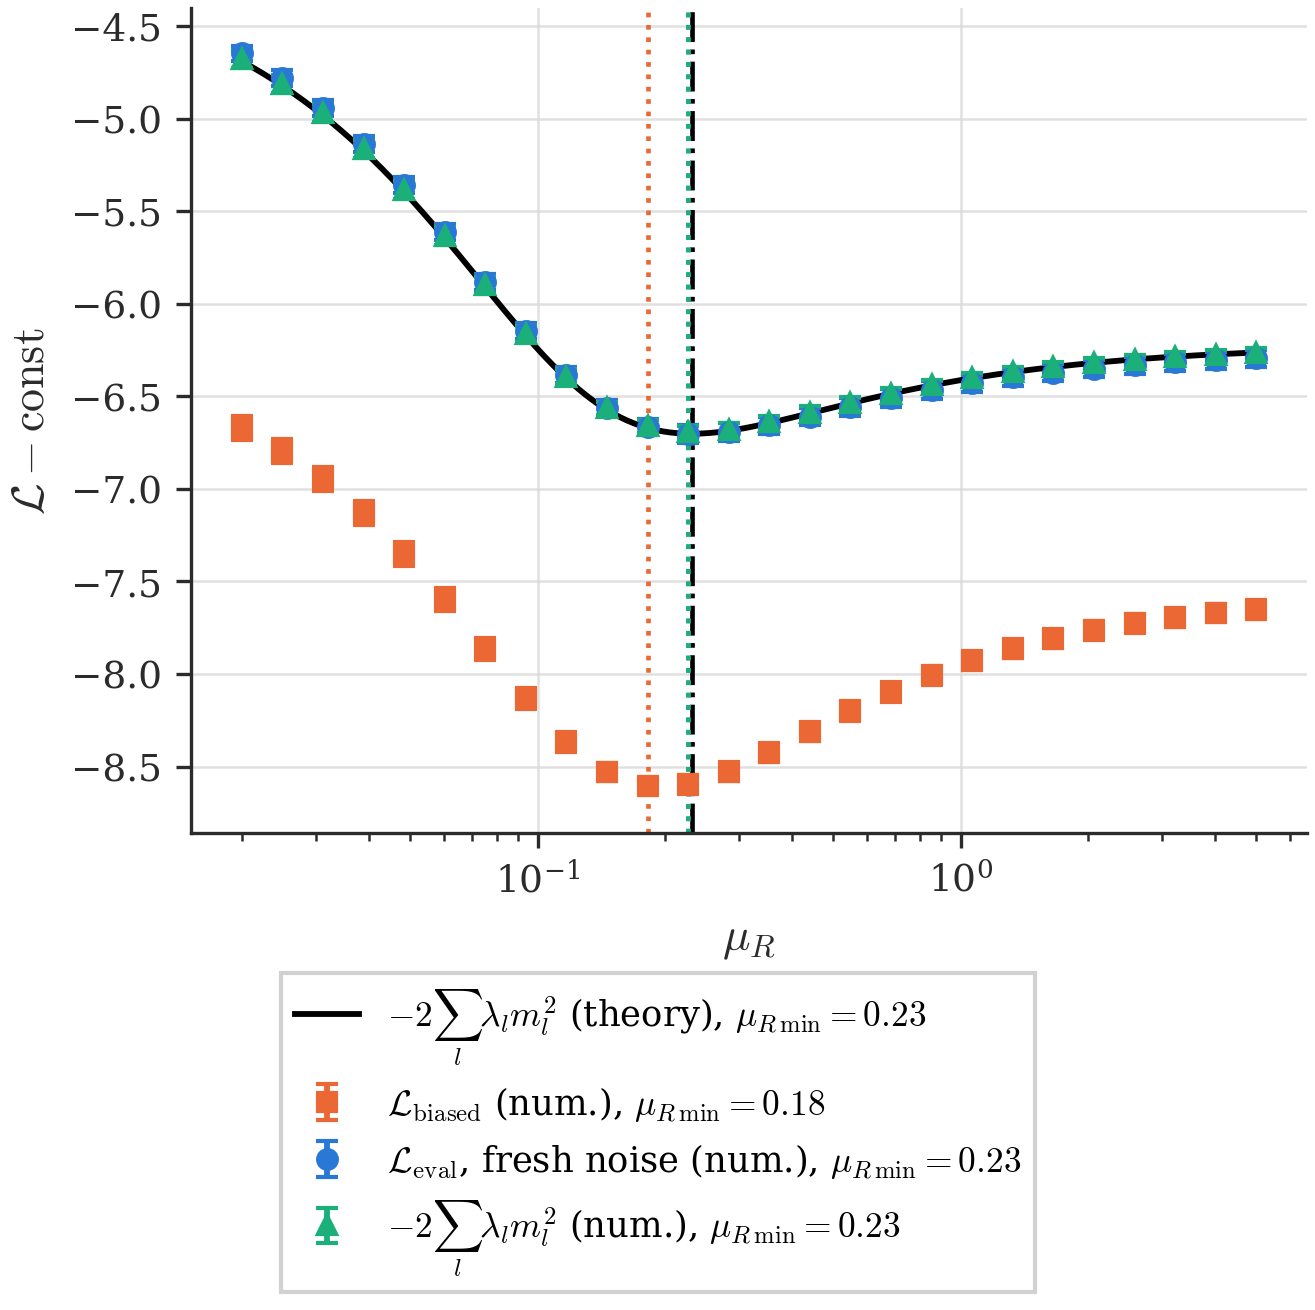
\includegraphics[width=\linewidth]{figures/loss_study/loss_biased_B_vs_mu_lam1=3.0_lam2=2.0_rho=0.5_report.png}
        \caption{Method B, as a function of $\mu_R$.}
        \label{fig:loss_opt_B}
    \end{subfigure}
    \caption{Evaluation Losses (up to a constant) as functions of the hyperparameter of each method, for $\lambda_1 = 3$, $\lambda_2 = 2$ and $\rho = 0.5$. Solid line: theoretical test loss $-2\sum_l\lambda_l m_l^2$. Dashed line: theoretical biased loss. Symbols: simulations with $n = \dots$, averaged over $\dots$ realisations (error bars: standard deviation), for the biased loss (squares), the loss evaluated on fresh noise (circles) and $-2\sum_l\lambda_l m_l^2$ computed from the measured overlaps (triangles). Vertical lines: minimisers of each curve, whose values are given in the legends. The theoretical biased loss of Method B is not computed.}
    \label{fig:loss_opt}
\end{figure}


\subsection{Comparison methods}
\begin{figure}[H]
    \centering
    \begin{subfigure}[t]{0.5\textwidth}
        \centering
        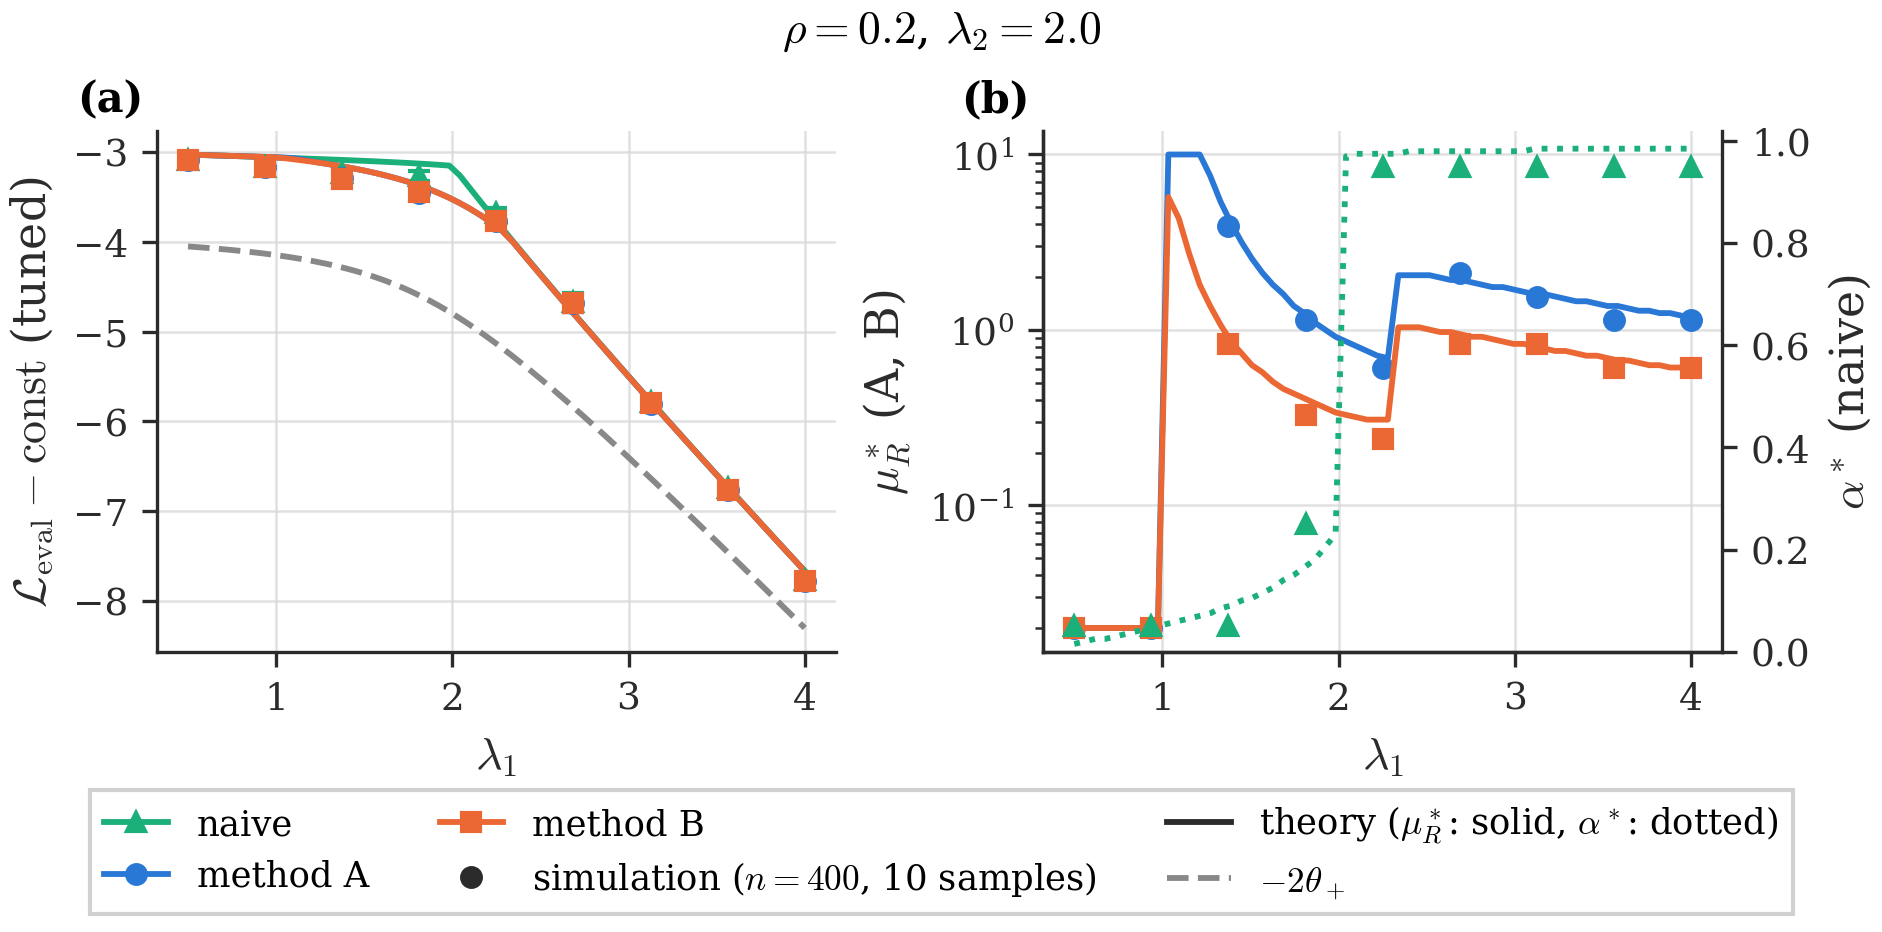
\includegraphics[width=\linewidth]{figures/loss_study/loss_unbiased_tuned_vs_lam1_lam2=2.0_rho=0.2_n=400_report.png}
        \caption{Naive method, as a function of $\alpha$.}
        \label{fig:loss_opt_naive}
    \end{subfigure}\hfill
    \begin{subfigure}[t]{0.5\textwidth}
        \centering
        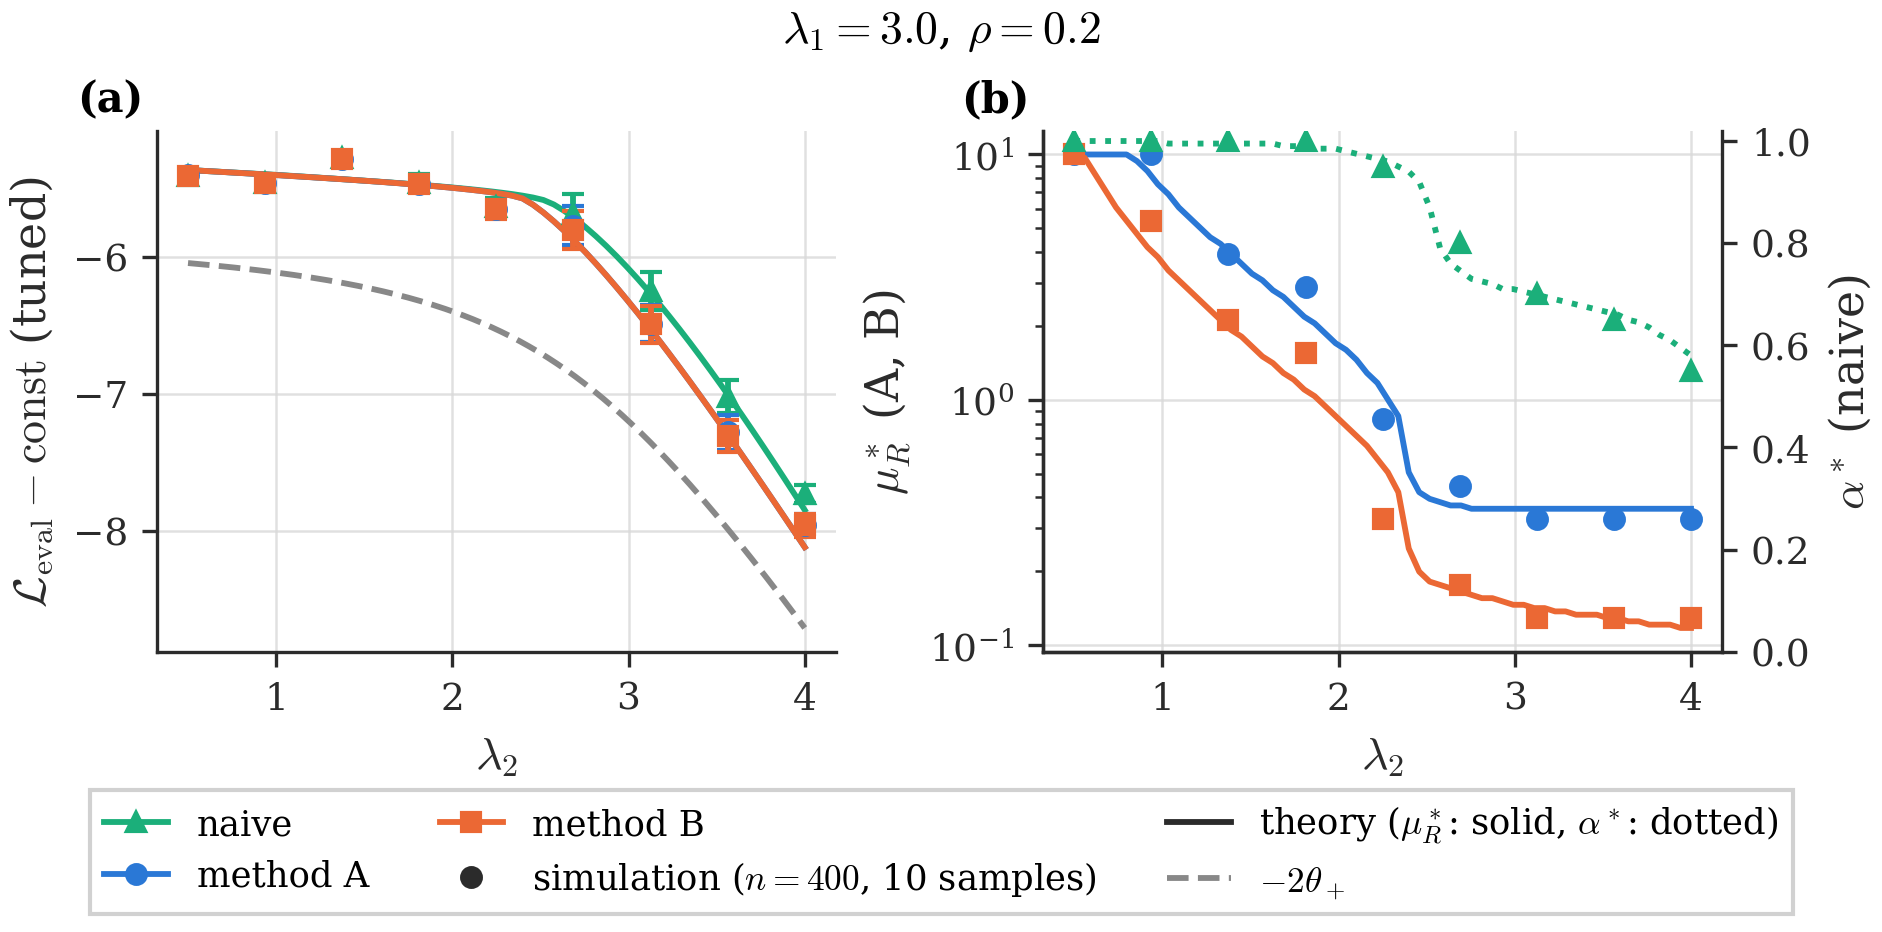
\includegraphics[width=\linewidth]{figures/loss_study/loss_unbiased_tuned_vs_lam2_lam1=3.0_rho=0.2_n=400_report.png}
        \caption{Method A, as a function of $\mu_R$.}
        \label{fig:loss_opt_A}
    \end{subfigure}\hfill
    \begin{subfigure}[t]{0.5\textwidth}
        \centering
        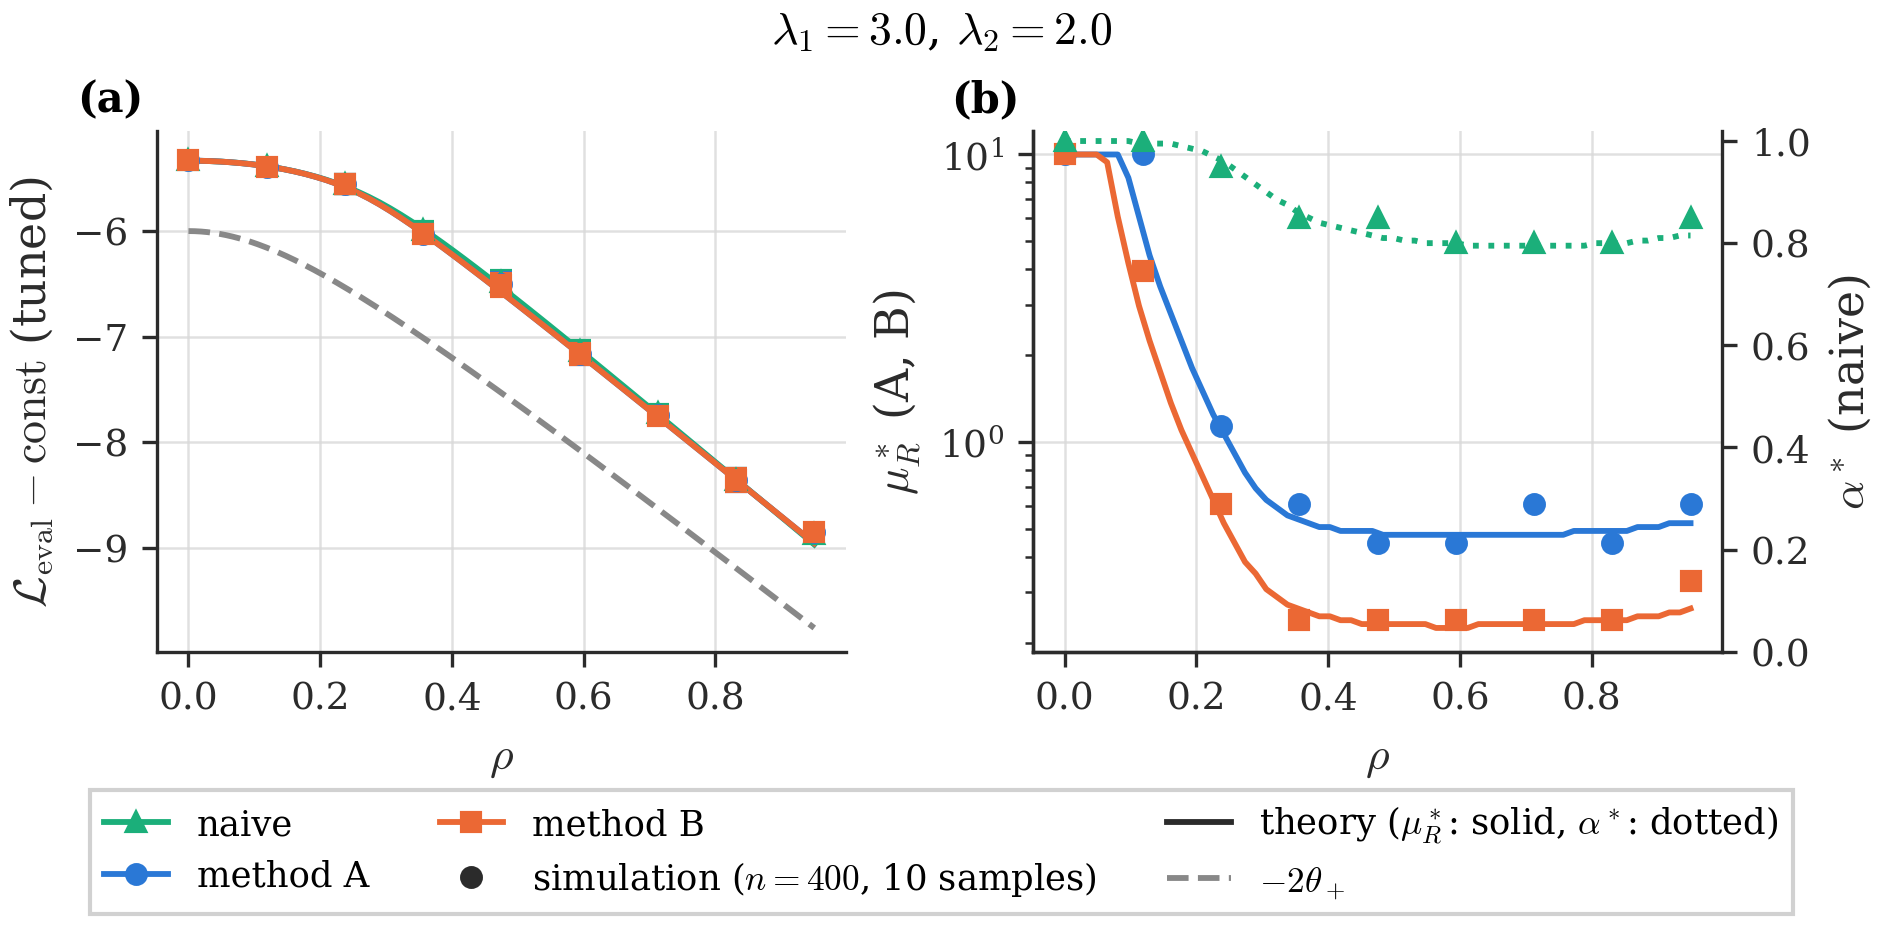
\includegraphics[width=\linewidth]{figures/loss_study/loss_unbiased_tuned_vs_rho_lam1=3.0_lam2=2.0_n=400_report.png}
        \caption{Method B, as a function of $\mu_R$.}
        \label{fig:loss_opt_B}
    \end{subfigure}
    \caption{}
    \label{fig:loss_opt}
\end{figure}
,
\begin{figure}[H]
    \centering
    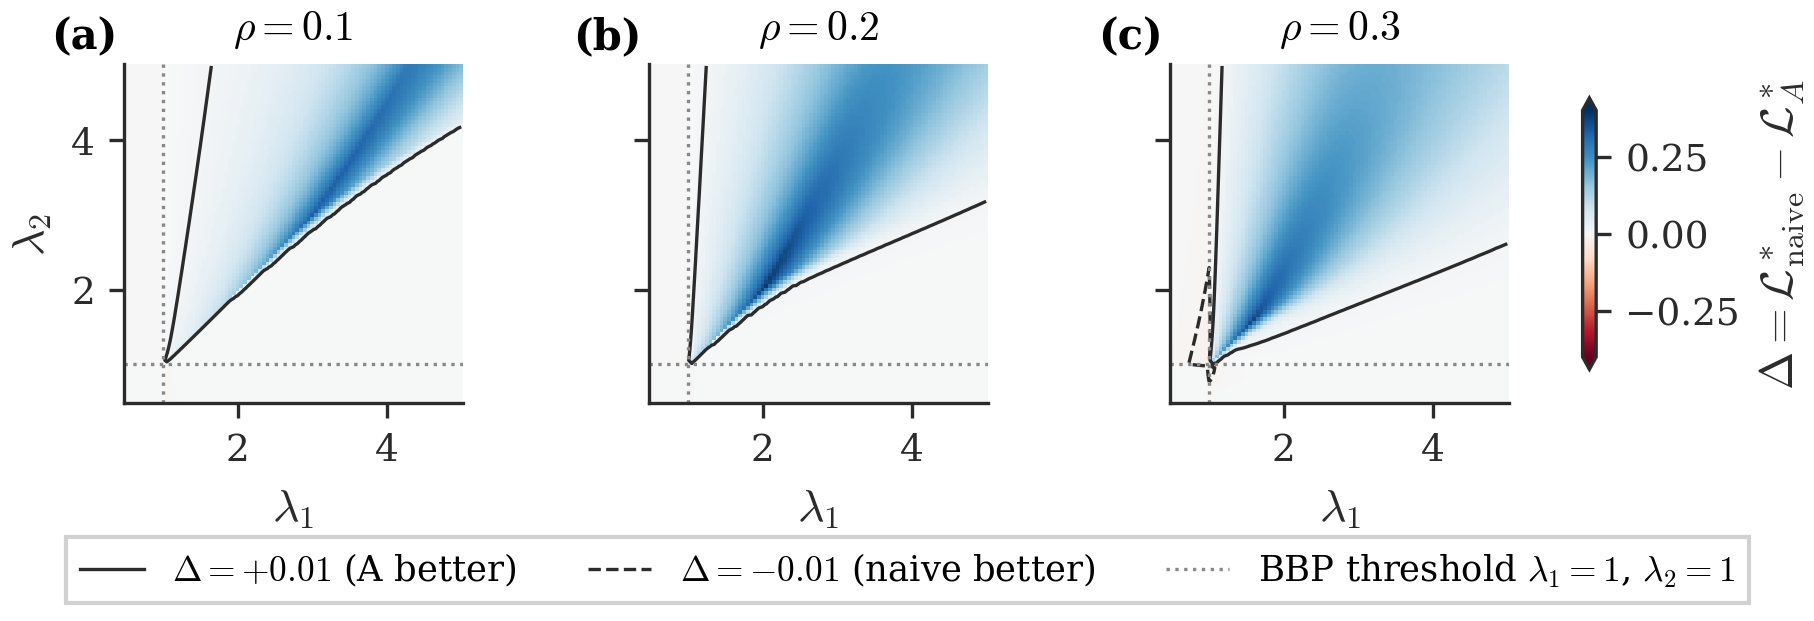
\includegraphics[width=0.9\linewidth]{figures/loss_study/heatmap_gap_naive_A_rho=0.1_0.2_0.3_report.png}
    \caption{Caption}
    \label{fig:placeholder}
\end{figure}
,
\begin{figure}[H]
    \centering
    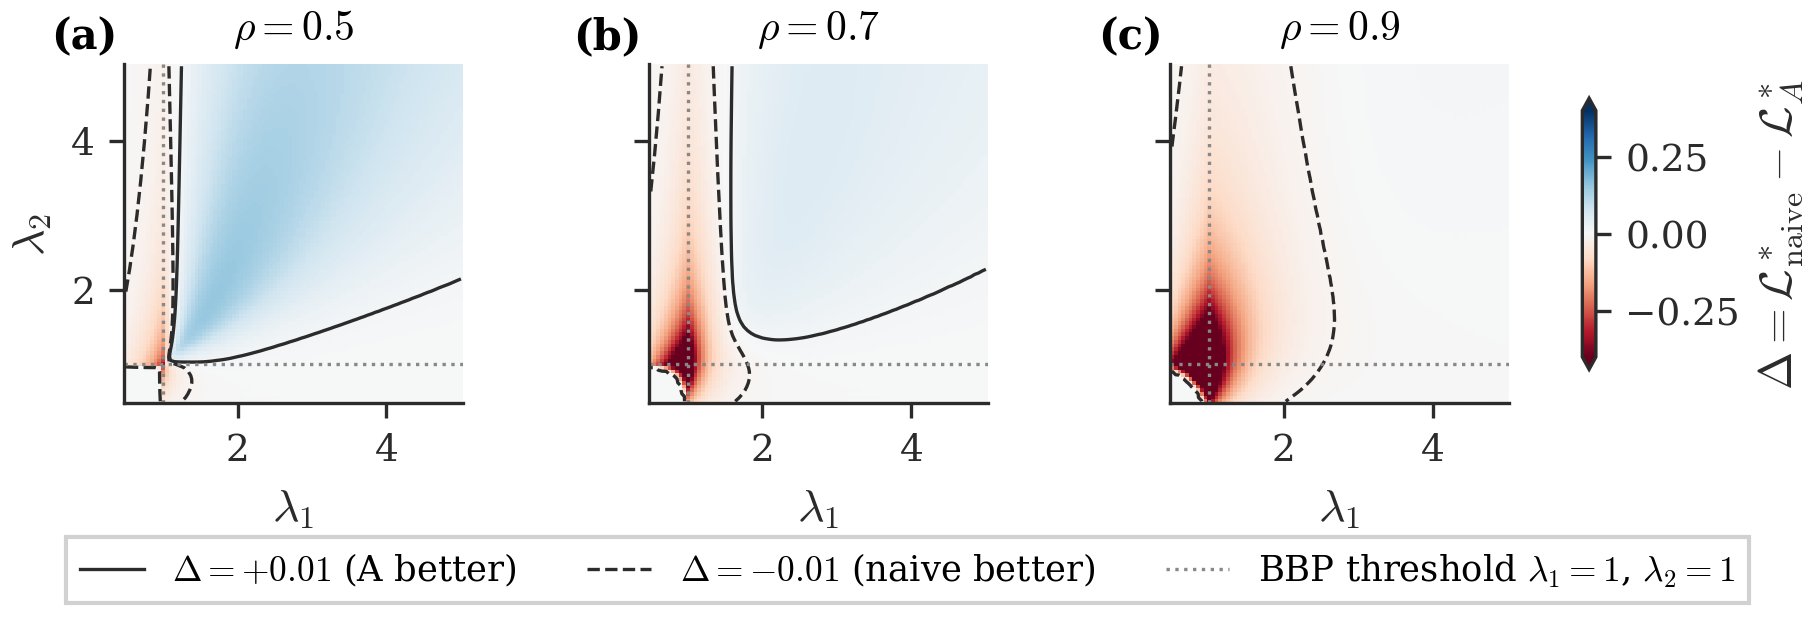
\includegraphics[width=0.9\linewidth]{figures/loss_study/heatmap_gap_naive_A_rho=0.5_0.7_0.9_report.png}
    \caption{Caption}
    \label{fig:placeholder}
\end{figure}
\begin{comment}
\subsubsection{Methode A: Optimal parameter}
Lets consider the method A estimator of our signals $\vect \hat x _A \equiv \vect \hat x _A(\mu_R) $. 

The condition eq.\ref{eq:mu_opt} on optimal regularization parameter $\mu_R^*$ is then:

\begin{equation}
    \boxed{
-4\left(\frac{\partial\vect{\hat x}_A(\mu_R^*)}{\partial\mu_R}\right)^T
\left(
\rdmmat Y_1+\rdmmat Y_2
-2\rdmmat I_n
\right)\vect{\hat x}_A (\mu_R^*) = 0.
}
\end{equation}

Let us consider the Method~A estimator, $\hat{\vect x}_A\equiv\hat{\vect x}_A(\mu_R)$ and consider the unormalized estimator $\Tilde{\vect x}_A$.

The optimality condition is therefore:
\[
\boxed{
\big(\partial \mu_R\Tilde{\vect x}_A\big)^{\,T}
\left[
Y-\frac{
\Tilde{\vect x}_A^{\,T}Y\Tilde{\vect x}_A
}{
\Tilde{\vect x}_A^{\,T}\Tilde{\vect x}_A
}
\rdmmat I_3
\right]
\Tilde{\vect x}_A=0.
}
\]

where $\vect v_{\max}$, $\widetilde{\vect v}$ and $\partial_{\mu_R}\widetilde{\vect v} = \frac{\partial \vect \Tilde v}{\partial \mu_R}$
are given in the paragraph \ref{sec:v_max_methodeA}.
The derivation of this condition is given in Annexe \ref{an:mu_rcond}.

\end{comment}




\section{Next step}
\begin{itemize}
    \item Numerics method A and B: phase diagram, overlap 2D, overlap 1D (transition)
    \item Numerics: optimal param $\mu_R$ research for methode A (Eval Loss vs mu)
    \item Numerics: Comparison of methods with Evaluation Loss
    \item Simpliphy 
    \item why B rank 2 and not 3, meme num peut etre
    \item diagram phase matrice A uniquement 
\end{itemize}

% macros compatible with the notation of the original notes




\newpage

\bibliographystyle{plain}
\bibliography{references}


\newpage
\appendix
\section{BBP transitions}
\subsection{BBP transition: rank one perturbation}
\begin{proof} 
    We consider
    \[
    Y = a\, x_1 x_1^T + W, \qquad W \sim \mathrm{GOE}, \qquad \|x_1\| = 1, \qquad a > 0.
    \]
    \paragraph{Top eigenvalue}
    
    The eigenvalues $z$ of $Y$ satisfy
    \[
    \det(z I - Y) = 0
    \]
    and we look for eigenvalues outside the semicircle, i.e.\ $z \notin [-2,2]$. In that case $\det(z I - W) \neq 0$, so we can write
    \[
    \det\left[ (z I - W)\left( I - a\, (z I - W)^{-1} x_1 x_1^T \right) \right] = 0
    \]
    We define the resolvent
    \[
    \mathrm{Res}(z) = (z I - W)^{-1} 
    \]
    Since $\det(z I - W) \neq 0$, we need $\det\left( I - a\, \mathrm{Res}(z)\, x_1 x_1^T \right) = 0$. \\
    Using
    \[
    \det(I - AB) = \det(I - BA)
    \]
    with $A = a\, \mathrm{Res}(z)\, x_1$ and $B = x_1^T$, we obtain
    \[
    a\, x_1^T\, \mathrm{Res}(z)\, x_1 = 1
    \]
    As W is real and symetric, we can write it sum lambdai ui ui with the ui orthogonal eigenvectors. The zI -  W has the same eigenvectors with eigenvalues z - lambdai, in a certain basis, this matrix is diagonal and we can inverse it givin the next equation. So the revolvent projects on u and multiplies by the factor 1/ z - lambdai.
    We expand $\mathrm{Res}(z)$ in the eigenbasis of $W$. Let $\lambda_i$ be the eigenvalues of $W$ and $u_i$ the associated orthonormal eigenvectors. Then
    \[
    \mathrm{Res}(z) = \sum_{i=1}^{N} \frac{u_i u_i^T}{z - \lambda_i}
    \]
    so
    \[
    x_1^T\, \mathrm{Res}(z)\, x_1 = \sum_{i=1}^{N} \frac{(x_1 \cdot u_i)^2}{z - \lambda_i}
    \]
    In mean, (could also say as W is GOE is rotation invariant, so applying a rotation doesn't change the eigenvalues) $x_1$ is uniform in all directions of the eigenbasis of $W$ as $W$ is GOE. Hence for $N \gg 1$,
    \[
    (x_1 \cdot u_i)^2 \to \frac{1}{N}
    \]
    and
    \[
    x_1^T\, \mathrm{Res}(z)\, x_1 = \frac{1}{N} \sum_{i=1}^{N} \frac{1}{z - \lambda_i} = S_W(z),
    \]
    where $S_W(z)$ is the Stieltjes transform of the empirical spectral distribution of $W$. CITER COURS DE SPOC ICI\\
    For a probability measure $\mu$ on $\mathbb{R}$ and $z$ outside its support, the Stieltjes transform is
    \[
    S_\mu(z) = \int \frac{d\mu(\lambda)}{z - \lambda} .
    \]
    For the empirical spectral distribution of $W$,
    \[
    \hat{\mu}_N = \frac{1}{N} \sum_{i=1}^{N} \delta_{\lambda_i},
    \]
    We know that the empirical spectral distribution converges to $\mu_{sc}$, the semicircle law:
    \[
    d\mu_{sc}(\lambda) = \frac{1}{2\pi} \sqrt{4 - \lambda^2}\; \mathbf{1}_{[-2,2]}(\lambda)\, d\lambda
    \]
    Therefore
    \[
    S_W(z) \to \frac{1}{2\pi} \int_{-2}^{2} \frac{\sqrt{4 - \lambda^2}}{z - \lambda}\, d\lambda
    \]
    With the change of variable $\lambda = 2 \cos \phi$, $\phi \in [0, \pi]$, we have $d\lambda = -2 \sin\phi\, d\phi$ and $\sqrt{4 - \lambda^2} = 2 \sin \phi$, so
    \[
    \frac{1}{2\pi} \int_{-2}^{2} \frac{\sqrt{4 - \lambda^2}}{z - \lambda}\, d\lambda
    = \frac{2}{\pi} \int_{0}^{\pi} \frac{\sin^2 \phi}{z - 2 \cos \phi}\, d\phi
    = \frac{z - \sqrt{z^2 - 4}}{2}, \qquad z > 2 .
    \]
    \\
    Hence $z$ is solution of
    \[
    a\, \frac{z - \sqrt{z^2 - 4}}{2} = 1
    \]
    This gives $z - \dfrac{2}{a} = \sqrt{z^2 - 4}$, so
    \[
    \left( z - \frac{2}{a} \right)^2 = z^2 - 4
    \quad \Longleftrightarrow \quad
    - \frac{4 z}{a} + \frac{4}{a^2} = -4
    \quad \Longleftrightarrow \quad
    z = a + \frac{1}{a} .
    \]
    Moreover, $z - \dfrac{2}{a} = \sqrt{z^2-4} \geq 0$ requires $a - \dfrac{1}{a} \geq 0$, and $z \geq 2$, which gives $a \geq 1$.\\
    We then arrive to the result that
    \[
    \boxed{
    z = a + \frac{1}{a} \quad \text{if } a \geq 1
    }
    \]
    For $a > 1$, $Y$ has an eigenvalue $z = a + 1/a > 2$ outside the bulk $[-2,2]$. For $a \leq 1$, there is no solution with $z > 2$ and the largest eigenvalue of $Y$ sticks to the edge of the semicircle at $2$.
    \paragraph{Overlap}
    Lets define $\vect u(a)$, the top eigenvector of $\vect Y$ associated with the eigenvalue found earlier $z(a)$ (with a the signal to noise ration), so that $\vect Y \vect u(a) = z(a) \vect u(a) $. Derinving by $a$, we get:
    \[
    \frac{\mathrm{d \vect Y(a)}}{\mathrm{d} a} \vect u(a) + \vect Y(a) \frac{\mathrm{d} \vect u(a)}{\mathrm{d} a} = \frac{\mathrm{d} z(a)}{\mathrm{d} a} \vect u(a) + z(a) \frac{\mathrm{d} \vect u(a)}{\mathrm{d} a}
    \]
    We have $\frac{\mathrm{d \vect Y(a)}}{\mathrm{d} a} = \frac{\mathrm{d}}{\mathrm{d} a} (a\, x_1 x_1^T + W) = x_1 x_1^T$. Left multiplying by $\vect u(a) ^\top$ and since $\vect u(a)^\top \vect Y = z(a) \vect u(a)^\top$ :
    \[
    (\vect x_1 \cdot \vect u(a))^2 = \frac{\mathrm{d} z(a)}{\mathrm{d} a}
    \]
    Considering the limit $N>>1$:
    
    \[
        m = |< \vect x_1 , \vect u(a)>|= \begin{cases}
        0 & \text{if } a \le 1,\\[0.3em]
        \sqrt{1-a^{-2}} & \text{if } a > 1.
    \end{cases}
    \]
    \label{proof:BBP1}
    
\end{proof}

\subsection{Proof of the BBP transition for $k$ spikes}\label{proof:BBP_k_spikes}

We use the setting of Section~\ref{sec:model}: $\rdmmat Y=\rdmmat P+\rdmmat W+c\rdmmat I_n$, with $\rdmmat P=\rdmmat E\rdmmat B\rdmmat E^T$, $\rdmmat E=(\vect e_1\;\dots\;\vect e_k)$ and $\rdmmat B$ symmetric with eigenvalues $\theta_1>\dots>\theta_k>0$ (assumed distinct and positive). Note that we only need \emph{some} orthonormal basis $(\vect e_i)$ of $\mathrm{span}(\vect x_1,\dots,\vect x_k)$: the eigenvalues of $\rdmmat B$ are the non-zero eigenvalues of $\rdmmat P$, whatever the basis. Since $\rdmmat Y-c\rdmmat I_n$ has the same eigenvectors as $\rdmmat Y$ and eigenvalues shifted by $c$, we take $c=0$ and add $c$ at the end.

\begin{proof}[Proof of eq.~\eqref{eq:BBP-k-spikes}]
Let $z$ be an eigenvalue of $\rdmmat Y$ with $z\notin[-2,2]$, and $\mathrm{Res}(z)=(z\rdmmat I_n-\rdmmat W)^{-1}$. Exactly as in the two-spike case,
\[
\det(z\rdmmat I_n-\rdmmat Y)=0
\;\Rightarrow\;
\det\big(\rdmmat I_n-\mathrm{Res}(z)\rdmmat E\rdmmat B\rdmmat E^T\big)=0
\;\Rightarrow\;
\det\big(\rdmmat I_k-\rdmmat B\,\rdmmat E^T\mathrm{Res}(z)\rdmmat E\big)=0,
\]
where we used $\det(\rdmmat I_n-\rdmmat X\rdmmat Y)=\det(\rdmmat I_k-\rdmmat Y\rdmmat X)$ with $\rdmmat X=\mathrm{Res}(z)\rdmmat E$ and $\rdmmat Y=\rdmmat B\rdmmat E^T$ (the $k\times k$ matrix to study is $\rdmmat E^T\mathrm{Res}(z)\rdmmat E$, with entries $\vect e_i^T\mathrm{Res}(z)\vect e_j$).

Since $\rdmmat W$ is orthogonally invariant and $(\vect e_i)$ is orthonormal, as for two spikes
\[
\vect e_i^T\mathrm{Res}(z)\vect e_i\to S_W(z),\qquad \vect e_i^T\mathrm{Res}(z)\vect e_j\to0\ (i\neq j),
\qquad\text{i.e.}\qquad
\rdmmat E^T\mathrm{Res}(z)\rdmmat E\to S_W(z)\,\rdmmat I_k .
\]
The equation becomes
\[
\det\big(\rdmmat I_k-S_W(z)\rdmmat B\big)=0
\;\Longleftrightarrow\;
\prod_{l=1}^k\big(1-\theta_l S_W(z)\big)=0,
\]
because $\rdmmat B$ has eigenvalues $\theta_1,\dots,\theta_k$. So the $k$ correlated spikes decouple into $k$ independent equations $S_W(z)=1/\theta_l$. Each one is solved as in the rank-one case: from $S_W^2-zS_W+1=0$ we get $z=S_W+1/S_W$, hence
\[
z=\theta_l+\frac1{\theta_l}\quad\text{if }\theta_l>1,
\]
and there is no solution outside $[-2,2]$ if $\theta_l\le1$ (the eigenvalue sticks to the edge of the bulk, $\lambda\to2$). Adding back $c$ gives eq.~\eqref{eq:BBP-k-spikes}.
\end{proof}

\subsubsection{Proof of the overlaps}\label{proof:BBP_k_overlaps}

Let $\theta_l>1$, $\lambda=\lambda^{\mathrm{out}}_l$ the corresponding outlier of $\rdmmat Y$ and $\vect u=\vect u_l$ its unit eigenvector. We use $S_W(z)=\frac{z-\sqrt{z^2-4}}{2}$ and, by differentiating $S_W^2-zS_W+1=0$,
\[
S_W'(z)=\frac{S_W(z)}{2S_W(z)-z}.
\]
At $z_l=\theta_l+1/\theta_l$ we have $S_W(z_l)=1/\theta_l$ and $2S_W-z=\frac{1-\theta_l^2}{\theta_l}$, so $S_W'(z_l)=\frac1{1-\theta_l^2}$.
\begin{comment}
\begin{proof}[Proof of eq.~\eqref{eq:BBP_overlap_k_spikes}]
From $(\lambda\rdmmat I-\rdmmat W)\vect u=\rdmmat E\rdmmat B\rdmmat E^T\vect u$, setting $\vect w:=\rdmmat B\rdmmat E^T\vect u\in\R^k$:
\[
\vect u=\mathrm{Res}(\lambda)\rdmmat E\vect w,
\qquad
\rdmmat E^T\vect u=\rdmmat E^T\mathrm{Res}(\lambda)\rdmmat E\,\vect w\simeq S_W(z_l)\,\vect w=\frac{\vect w}{\theta_l}.
\]
\emph{Direction of $\vect w$.} Plugging into the definition of $\vect w$: $\vect w=\rdmmat B\rdmmat E^T\vect u\simeq\frac1{\theta_l}\rdmmat B\vect w$, i.e. $\rdmmat B\vect w\simeq\theta_l\vect w$. Since $\theta_l$ is a simple eigenvalue of $\rdmmat B$, $\vect w\parallel\tilde{\vect v}_l$.

\emph{Norm of $\vect w$.} Using $\mathrm{Res}'(z)=-\mathrm{Res}(z)^2$ and $\rdmmat E^T\mathrm{Res}'(z)\rdmmat E\to S_W'(z)\rdmmat I_k$,
\[
1=\norm{\vect u}^2=\vect w^T\rdmmat E^T\mathrm{Res}(\lambda)^2\rdmmat E\,\vect w\simeq-S_W'(z_l)\norm{\vect w}^2=\frac{\norm{\vect w}^2}{\theta_l^2-1}
\;\Rightarrow\;\norm{\vect w}^2\simeq\theta_l^2-1 .
\]

\emph{Overlap.} Since $\vect v_{l'}=\rdmmat E\tilde{\vect v}_{l'}$,
\[
\langle\vect u,\vect v_{l'}\rangle=\tilde{\vect v}_{l'}^T\rdmmat E^T\vect u\simeq\frac1{\theta_l}\tilde{\vect v}_{l'}^T\vect w
=\pm\frac{\sqrt{\theta_l^2-1}}{\theta_l}\,\delta_{ll'},
\]
because $\vect w\parallel\tilde{\vect v}_l$ and the $\tilde{\vect v}_{l'}$ are orthonormal. Squaring gives $\delta_{ll'}\big(1-\theta_l^{-2}\big)$.
\end{proof}

\begin{remark}[Without resolvent: Hellmann--Feynman]
Fix the $\vect v_l$ and let $\rdmmat Y(\boldsymbol\theta)=\rdmmat W+\sum_l\theta_l\vect v_l\vect v_l^T$. Differentiating $\rdmmat Y\vect u_j=\lambda_j\vect u_j$ and multiplying by $\vect u_j^T$ gives $\partial\lambda_j/\partial\theta_l=\langle\vect u_j,\vect v_l\rangle^2$. Since $\lambda_j\to\theta_j+1/\theta_j$ depends on $\theta_j$ only,
$\langle\vect u_j,\vect v_l\rangle^2\to\delta_{jl}\big(1-\theta_j^{-2}\big)$.
\end{remark}
\end{comment}
\begin{remark}[Alternative argument: Hellmann--Feynman]
Fix $\rdmmat W$ and the unit vectors $\vect v_1,\dots,\vect v_k$, and consider
\[
\rdmmat Y(\boldsymbol\theta)=\rdmmat W+\sum_{l=1}^k\theta_l\vect v_l\vect v_l^T,
\qquad \boldsymbol\theta\in D:=\{\theta_1>\dots>\theta_k>1\}.
\]
Let $\lambda_1(\boldsymbol\theta)\ge\lambda_2(\boldsymbol\theta)\ge\cdots$ be the eigenvalues of $\rdmmat Y(\boldsymbol\theta)$ and $\vect u_j$ unit eigenvectors.

\smallskip
\noindent\emph{Step 1: Hellmann--Feynman formula.}
If $\lambda_j$ is a simple eigenvalue, it is differentiable in $\boldsymbol\theta$. Differentiating $\rdmmat Y\vect u_j=\lambda_j\vect u_j$ with respect to $\theta_l$ gives
\[
\vect v_l\vect v_l^T\vect u_j+\rdmmat Y\,\partial_{\theta_l}\vect u_j=(\partial_{\theta_l}\lambda_j)\vect u_j+\lambda_j\,\partial_{\theta_l}\vect u_j .
\]
Multiplying on the left by $\vect u_j^T$ and using $\vect u_j^T\rdmmat Y=\lambda_j\vect u_j^T$, the terms in $\partial_{\theta_l}\vect u_j$ cancel, so
\[
\frac{\partial\lambda_j}{\partial\theta_l}=\langle\vect u_j,\vect v_l\rangle^2 .
\]
Similarly, if $\lambda_j>\lambda_{j+1}$, then $\Lambda_j:=\lambda_1+\dots+\lambda_j$ is differentiable and
\[
\frac{\partial\Lambda_j}{\partial\theta_l}=\sum_{i\le j}\langle\vect u_i,\vect v_l\rangle^2 .
\]
This is the case with high probability on $D$, since the outliers are separated from each other and from the bulk.

\smallskip
\noindent\emph{Step 2: convergence of the derivatives.}
By Ky Fan's principle, $\Lambda_j(\boldsymbol\theta)=\max_{\rdmmat Q^T\rdmmat Q=\rdmmat I_j}\mathrm{tr}\big(\rdmmat Q^T\rdmmat Y(\boldsymbol\theta)\rdmmat Q\big)$ is a maximum of affine functions of $\boldsymbol\theta$, hence convex. For $\boldsymbol\theta\in D$ and $j\le k$, the eigenvalue convergence $\lambda_i\to\theta_i+\theta_i^{-1}$ gives, almost surely,
\[
\Lambda_j(\boldsymbol\theta)\longrightarrow \Lambda_j^\infty(\boldsymbol\theta):=\sum_{i\le j}\Big(\theta_i+\frac1{\theta_i}\Big).
\]
(Convergence holds a.s.\ simultaneously for all $\boldsymbol\theta$ in a countable dense subset of $D$, and then, by convexity, for all $\boldsymbol\theta\in D$.)
The limit $\Lambda_j^\infty$ is $C^1$ on $D$. A classical result on convex functions (e.g.\ Rockafellar, \emph{Convex Analysis}, Thm.~25.7) states that if convex functions $f_n$ converge pointwise on an open convex set to a function $f$ differentiable at $\boldsymbol\theta$, then $\nabla f_n(\boldsymbol\theta)\to\nabla f(\boldsymbol\theta)$. Hence, for every $\boldsymbol\theta\in D$,
\[
\sum_{i\le j}\langle\vect u_i,\vect v_l\rangle^2=\frac{\partial\Lambda_j}{\partial\theta_l}
\longrightarrow\frac{\partial\Lambda_j^\infty}{\partial\theta_l}
=\mathbf 1_{\{l\le j\}}\Big(1-\frac1{\theta_l^2}\Big).
\]

\smallskip
\noindent\emph{Step 3: conclusion.}
Taking the difference between $j$ and $j-1$ (with $\Lambda_0:=0$),
\[
\langle\vect u_j,\vect v_l\rangle^2
=\frac{\partial\Lambda_j}{\partial\theta_l}-\frac{\partial\Lambda_{j-1}}{\partial\theta_l}
\longrightarrow\big(\mathbf 1_{\{l\le j\}}-\mathbf 1_{\{l\le j-1\}}\big)\Big(1-\frac1{\theta_l^2}\Big)
=\delta_{jl}\Big(1-\frac1{\theta_j^{2}}\Big).
\]
\end{remark}
\subsubsection{Proof of the overlap with the signals}

Since $\vect x_i=\sum_{l}q_i^l\vect v_l$, we have $\langle\vect u_l,\vect x_i\rangle=\sum_{l'}q_i^{l'}\langle\vect u_l,\vect v_{l'}\rangle$. By eq.~\eqref{eq:BBP_overlap_k_spikes} only $l'=l$ survives, so
\[
\big|\langle\vect u_l,\vect x_i\rangle\big|\to|q_i^l|\sqrt{1-\frac1{\theta_l^2}},
\]
which is eq.~\eqref{eq:overlap_signal_k-spikes}. (In your notes the sum should read $\langle\vect u_l,\vect v_{l'}\rangle$, not $\langle\vect u_{l'},\vect v_{l'}\rangle$.)

%\paragraph{Factorised form:}

\section{EWC: Fisher matrix and stationarity condition}

\subsection{Derivation of the Fisher matrix}\label{adix:fisher}

We consider a single task, $\vect Y = \lambda\,\vect x\vect x^\top + \vect W$ (for the first task of Section~\ref{sec:ewc}, $\lambda = \lambda_1$), with the misspecified loss
\[
    \mathcal{L}(\vect{x}) = -\tfrac{1}{4} \|\vect Y - \vect{x}\vect{x}^\top\|_F^2 .
\]
Its gradient is
\[
    \vect \nabla_x \mathcal{L}(\vect{x}) = (\vect Y - \vect{x} \vect{x}^\top) \vect{x} = \vect Z\vect{x},
    \qquad \vect Z := \vect Y - \vect{x} \vect{x}^\top ,
\]
so that, since $\vect Z^\top = \vect Z$,
\[
    \vect \nabla_x \mathcal{L}(\vect{x}) \vect \nabla_x \mathcal{L}(\vect{x})^\top = \vect Z \vect{x}\vect{x}^\top \vect Z ,
    \qquad
    \mathcal{F}_{\mathrm{MS}}(\vect{x}) = \mathbb{E}[\vect Z \vect{x}\vect{x}^\top \vect Z] .
\]
With $\vect Z = (\lambda - 1) \vect{x} \vect{x}^\top + \vect W$, where $\vect W$ is the bulk of the noise, a symmetric Gaussian Wigner matrix with $\mathbb{E}[W_{ij}]=0$ and $\mathbb{E}[W_{ij}^2]=\sigma^2=\frac{1}{n}$, the cross terms vanish and
\[
\mathbb{E} [\vect Z \vect{x} \vect{x}^\top \vect Z] = (\lambda - 1)^2 \vect{x} \vect{x}^\top + \mathbb{E}[\vect W \vect{x} \vect{x}^\top \vect W] .
\]
\begin{property} \label{prop:wigner_expectation}
\[
    \mathbb{E}[\vect W \vect A \vect W] = \sigma^2(\mathrm{Tr}(\vect A) \vect I + \vect A^\top).
\]
\end{property}
\noindent
Applying Prop.~\ref{prop:wigner_expectation} to $\vect A = \vect{x} \vect{x}^\top$ with $\|\vect{x}\| = 1$, i.e.\ $\mathrm{Tr}(\vect A) = 1$ and $\vect A^\top = \vect A$,
\[
\mathbb{E}[\vect W \vect{x} \vect{x}^\top \vect W] = \frac{1}{n}(\vect I + \vect{x} \vect{x}^\top),
\]
which gives the Fisher matrix used in Section~\ref{sec:ewc}:
\begin{equation}
    \mathcal{F}_{\mathrm{MS}}(\vect{x}) = (\lambda-1)^2\vect{x}\vect{x}^\top + \frac{1}{n}(\vect I + \vect{x} \vect{x}^\top) .
    \label{eq:fisher_ms}
\end{equation}

\subsection{Derivation of the EWC stationarity condition}\label{adix:ewc}
With the misspecified losses $\mathcal{L}_{i,\mathrm{MS}}(\vect{x}) = -\tfrac{1}{4} \|\vect Y_i - \vect{x}\vect{x}^\top\|_F^2$, of gradient $\vect \nabla \mathcal{L}_{i,\mathrm{MS}}(\vect{x}) = (\vect Y_i - \vect{x}\vect{x}^\top) \vect{x}$, the EWC loss is
\[
    \mathcal L_{\mathrm{EWC}}(\vect{x}) = \mathcal{L}_{2,\mathrm{MS}}(\vect{x}) +
    \mu_R (\vect{x} - \hat{\vect{x}}^{(1)})^\top \vect F_1(\vect{x} - \hat{\vect{x}}^{(1)}),
\]
with $\hat{\vect{x}}^{(1)}$ the optimizer of $\mathcal{L}_{1,\mathrm{MS}}$ on the first task only. Using $\vect F_1^\top=\vect F_1$,
\[
    \vect \nabla \mathcal L_{\mathrm{EWC}}(\vect{x})= (\vect Y_2 - \vect{x} \vect{x}^\top) \vect{x}+2\mu_R \vect F_1(\vect{x} - \hat{\vect x}^{(1)}) .
\]
We substitute $\|\vect{x}\|^2 = 1$ directly into the gradient (rather than enforcing it through a Lagrange multiplier at this stage), which linearises the stationarity condition in $\vect{x}$. The constraint is re-imposed afterwards through the Lagrange multiplier of Eq.~\eqref{eq:final_estimator_lagrange}. The gradient becomes
\[
 \vect \nabla \mathcal L_{\mathrm{EWC}}(\vect{x})= (\vect Y_2 - \vect I) \vect{x}+2\mu_R \vect F_1(\vect{x} - \hat{\vect x}^{(1)}),
\]
and the Hessian is
\[
    \mathcal{H}_{\mathrm{EWC}} = \vect \nabla \vect \nabla ^\top \mathcal{L}_{\mathrm{EWC}} = \vect Y_2 - \vect I  + 2 \mu_R \vect F_1 .
\]
The stationarity condition $\vect \nabla \mathcal L_{\mathrm{EWC}}(\vect{x})= 0$ then reads
\[
(\vect Y_2 - \vect I + 2 \mu_R \vect F_1) \vect{x}=2 \mu_R\vect F_1\hat{\vect x}^{(1)},
\]
which is the affine system $\vect A \vect{x} = \vect b$ of Eq.~\eqref{eq:stationary_condition}, with $\vect A = \mathcal{H}_{\mathrm{EWC}}$. Whenever $\vect A$ is invertible, it is solved by
\[
    \hat{\vect{x}}^{(2)} = \vect A^{-1}\vect b = 2\mu_R\,\vect R_{\vect A}(0)\,\vect F_1 \hat{\vect x}^{(1)},
\]
with $\vect R_{\vect A}(z) = (\vect A - z\vect I)^{-1}$ the resolvent of $\vect A$, as in Section~\ref{sec:ewc}.

\section{Naive method}\label{proof:naive}
The observable splits into a noise part and a low rank signal part:
\begin{equation}
    \rdmmat Y = \underbrace{a\,\vect{x_1}\vect{x_1}^T + b\,\vect{x_2}\vect{x_2}^T}_{=:\ \rdmmat P}
              + \underbrace{\alpha \rdmmat Z_1 + \sqrt{1-\alpha^2}\,\rdmmat Z_2}_{=:\ \rdmmat W}
    \qquad
    a := \alpha\lambda_1, \quad b := \sqrt{1-\alpha^2}\,\lambda_2
    \label{eq:Y-split}
\end{equation}
Since $\rdmmat Z_1$ and $\rdmmat Z_2$ are independent with entries of variance $1/n$, the entries of $\rdmmat W$ are Gaussian with variance $(\alpha^2 + 1 - \alpha^2)/n = 1/n$: the noise $\rdmmat W$ is again a Wigner matrix. So \eqref{eq:Y-split} is a rank-two spiked Wigner model whose spike matrix $\rdmmat P$ carries all the dependence on $\alpha$, $\lambda_1$, $\lambda_2$ and $\rho$. We can then compute its spectrum in closed form from section \ref{sec:general_results} with $P$ and $c=0$.

Expanding $\rdmmat P$ in an orthonormal basis $(e_1, e_2)$ of $\mathrm{span}(x_1, x_2)$ defined by
    \[
    x_1 = e_1, \qquad x_2 = \rho\, e_1 + \sqrt{1-\rho^2}\, e_2 .
    \]
    We have
    \[
    \rdmmat P = (a + b\rho^2)\, \vect e_1 \vect e_1^T + b\rho\sqrt{1-\rho^2}\, ( \vect e_1 \vect e_2^T + \vect e_2 \vect e_1^T) + b(1-\rho^2)\, \vect e_2 \vect e_2^T ,
    \]
    so that
    \[
    \vect P = \vect E \vect B \vect E^T, \qquad \vect E = (\vect e_1 \;\; \vect e_2),
    \]
    where $\vect E$ is the $N \times 2$ matrix with columns $\vect e_1, \vect e_2$ and
    \[
    \vect B = \begin{pmatrix} a + b\rho^2 & b\rho\sqrt{1-\rho^2} \\ b\rho\sqrt{1-\rho^2} & b(1-\rho^2) \end{pmatrix}
    \]

\paragraph{Eigenvalues and eigenvectors of the signal matrix $\rdmmat P$}
From section \ref{sec:model}, the non zero eigenvalues of $\rdmmat P$ are the same as $\rdmmat B$. Leading to the eigenvalues
\begin{equation}
    \boxed{\;
    \theta_\pm = \frac{a+b}{2} \pm \sqrt{\Big(\frac{a-b}{2}\Big)^2 + ab\,\rho^2}
    \;}
    \qquad
    a = \alpha\lambda_1, \quad b = \sqrt{1-\alpha^2}\,\lambda_2
    \label{eq:theta-pm}
\end{equation}
The discriminant is non-negative, so $\theta_\pm \in \mathbb{R}$. \\
For this method, our estimator is the top eigenvector of $\rdmmat Y$, and so only the top eigenvalue $\theta_+$ will be studied. Computing the top eigenvector of $\rdmmat B$ and expanding them in the $\R^n$ space, from section \ref{sec:model}, the top eigenvector of $\rdmmat P$ is:
\[
    \boxed{
    \vect v_+ = c_1^+\,\vect{x_1} + c_2^+\,\vect{x_2},
    \qquad
    \big(c_1^+,\, c_2^+\big) = \frac{\big(r,\, 1\big)}{\sqrt{r^2 + 2\rho\, r + 1}},
    \qquad
    r = \frac{\rho\, a}{\theta_+ - a} = \frac{\theta_+ - b }{b \; \rho}.
    }
\]
the full calculation of the eigenvectors is in Annex \ref{sec:eigenvect_naive}.
In the limit $N >> 1$, leading to:
\[
    q_1^+ = \langle \vect x_1, \vect v_+ \rangle = c_1^+ + \rho c_2^+ \qquad q_2^+ = \langle \vect x_2, \vect v_+ \rangle = c_2^+ + \rho c_1^+
\]


\paragraph{Overlap of the estimator with the signals.}
Then considering our estimator $\hat{\vect x}_{naive} := \vect u_+$ being the top eigenvector of the observation $\rdmmat Y$. From equation \ref{eq:overlap_signal_k-spikes}, and rewriting $q_1^+$ and $q_2^+$, the overlap with our signals are:

\begin{equation}
\boxed{
    m_1 := |\langle \hat{\vect x}_{naive}, \vect{x_1}\rangle| \xrightarrow[n\to\infty]{\text{a.s.}} \Bigg \lvert \frac{\theta_+}{a}c_1^+ \Bigg \rvert \; \sqrt{1-\theta_+^{-2}} }
    \qquad
    \boxed{
    m_2 := |\langle \hat{\vect x}_{naive}, \vect{x_2}\rangle| \xrightarrow[n\to\infty]{\text{a.s.}} \Bigg \lvert  \frac{\theta_+}{b}c_2^+  \Bigg \rvert \; \sqrt{1-\theta_+^{-2}} }
    \label{eq:m12-naive}
\end{equation}
for $\theta_+ > 1$, and $m_1, m_2 \to 0$ for $\theta_+ \le 1$.


\paragraph{Derivation of the signal matrix eigenvectors } \label{sec:eigenvect_naive}
We now derive the eigenvectors of $\rdmmat P$ in closed form. We assume $a, b > 0$ (i.e.\ $\alpha \in (0,1)$ and $\lambda_1, \lambda_2 > 0$) and $\rho \in [0,1)$, so that both $\theta_\pm$ are strictly positive. We introduce
\begin{equation}
    \Delta := \sqrt{\Big(\frac{a-b}{2}\Big)^2 + ab\,\rho^2},
    \qquad \text{so that} \qquad
    \theta_\pm = \frac{a+b}{2} \pm \Delta.
    \label{eq:Delta}
\end{equation}
We exclude the degenerate case $a = b$, $\rho = 0$, in which $\theta_+ = \theta_-$ and every vector of $\operatorname{span}(\vect{x_1},\vect{x_2})$ is an eigenvector.

%\paragraph{Going to the plane of the signals (méthode de Celia):} 
\noindent
Since the eigenvectors lie in $\operatorname{span}(\vect{x_1},\vect{x_2})$, we can express them in $\operatorname{span}(\vect{x_1},\vect{x_2})$. Let $\vect v$ be a unit eigenvector of $\rdmmat P$ with eigenvalue $\theta \neq 0$. Since
\begin{equation}
    \rdmmat P \vect v = a\,\langle \vect{x_1}, \vect v\rangle\,\vect{x_1} + b\,\langle \vect{x_2}, \vect v\rangle\,\vect{x_2} = \theta\,\vect v
\end{equation}
and we write
\begin{equation}
    \vect v = c_1\,\vect{x_1} + c_2\,\vect{x_2},
    \qquad
    \langle \vect{x_1}, \vect v\rangle = c_1 + \rho\, c_2,
    \qquad
    \langle \vect{x_2}, \vect v\rangle = \rho\, c_1 + c_2 .
    \label{eq:ansatz}
\end{equation}
Substituting into the eigenvalue equation and identifying the coefficients of $\vect{x_1}$ and $\vect{x_2}$ (which are linearly independent since $\rho < 1$) gives
\begin{equation}
    \begin{cases}
        a\,(c_1 + \rho\, c_2) = \theta\, c_1 ,\\[2pt]
        b\,(\rho\, c_1 + c_2) = \theta\, c_2 ,
    \end{cases}
    \label{eq:eig-system}
\end{equation}
A non-trivial solution exists if and only if $\theta \in \{\theta_+, \theta_-\}$, recovering \eqref{eq:theta-pm}. For $\rho > 0$ we have $(\theta_\pm - a)(\theta_\pm - b) = ab\rho^2 > 0$, so $\theta_\pm \neq a$, and the first row yields
\begin{equation}
    c_1 = r_\pm\, c_2,
    \qquad
    r_\pm := \frac{\rho\, a}{\theta_\pm - a} = \frac{\theta_\pm - b}{b\rho},
    \label{eq:ratio}
\end{equation}
where the two expressions for $r_\pm$ agree precisely because of the characteristic equation. For the same reason, the second row of \eqref{eq:eig-system} is then automatically satisfied.

%\paragraph{Normalization:} 
\noindent
We can then normalize the eigenvector, using that $\norm{\vect{x_1}} = \norm{\vect{x_2}} = 1$ and $\langle \vect{x_1},\vect{x_2}\rangle = \rho$,
\begin{equation}
    \norm{\vect v}^2 = c_1^2 + 2\rho\, c_1 c_2 + c_2^2
    = c_2^2\,\big( r_\pm^2 + 2\rho\, r_\pm + 1 \big) = 1
    \quad \Longrightarrow \quad
    c_2 = \pm \big( r_\pm^2 + 2\rho\, r_\pm + 1 \big)^{-1/2}
\end{equation}
The bracket is strictly positive, since $r^2 + 2\rho r + 1 = (r+\rho)^2 + 1 - \rho^2 > 0$.

%\paragraph{Final expression for the eigenvectors of the noiseless $\rdmmat P$:} 
\noindent
Combining \eqref{eq:ratio} with the normalization, the unit-norm eigenvectors of $\rdmmat P$ associated with $\theta_\pm$ are, up to an overall sign,
\begin{equation}
    \boxed{
    \hat{\vect v}_\pm = c_1^\pm\,\vect{x_1} + c_2^\pm\,\vect{x_2},
    \qquad
    \big(c_1^\pm,\, c_2^\pm\big) = \frac{\big(r_\pm,\, 1\big)}{\sqrt{r_\pm^2 + 2\rho\, r_\pm + 1}},
    \qquad
    r_\pm = \frac{\rho\, a}{\theta_\pm - a} .
    }
    \label{eq:v-final}
\end{equation}

%\paragraph{Overlaps of the noiseless eigenvectors with the signals:} 
\noindent
The overlaps of $\hat{\vect v}_\pm$ with the signals follow directly from \eqref{eq:ansatz} and \eqref{eq:eig-system}, since $c_1 + \rho c_2 = \theta c_1/a$ and $\rho c_1 + c_2 = \theta c_2/b$:
\begin{equation}
\boxed{
    \langle \hat{\vect v}_\pm, \vect{x_1}\rangle = \frac{\theta_\pm}{a}\, c_1^\pm}
    \qquad
    \boxed{
    \langle \hat{\vect v}_\pm, \vect{x_2}\rangle = \frac{\theta_\pm}{b}\, c_2^\pm}
    \label{eq:overlaps-signals}
\end{equation}
Eq. \eqref{eq:overlaps-signals} shows that the \emph{coefficients} $c_i^\pm$ (how much of each signal we put into the mixture) are not the same thing as the \emph{overlaps} $\langle \hat{\vect v}_\pm, \vect{x_i}\rangle$ (how much of each signal we actually see), because $\vect{x_1}$ and $\vect{x_2}$ are not orthogonal.

\medskip
\noindent
Multiplying the first relation in Eq. \eqref{eq:overlaps-signals} by $a\,\langle \hat{\vect v}_\pm, \vect{x_1}\rangle$, its second by $b\,\langle \hat{\vect v}_\pm, \vect{x_2}\rangle$, adding, and using the normalization $c_1^2 + 2\rho c_1 c_2 + c_2^2 = 1$, we get
\begin{equation}
\boxed{
    \theta_\pm \;=\; \hat{\vect v}_\pm^{\,T}\, \rdmmat P\, \hat{\vect v}_\pm
    \;=\; a\,\langle \hat{\vect v}_\pm, \vect{x_1}\rangle^2 + b\,\langle \hat{\vect v}_\pm, \vect{x_2}\rangle^2}
    \label{eq:theta-pm-relation}
\end{equation}

\section{Hessian of the EWC loss and Methods A and B}\label{adix:hessian}
\subsection{Method A and B: Matrix $\rdmmat A$}\label{tab:coefficients_beta_A(xP1)}

\begin{table}[htbp]
    \centering
    
    
    \renewcommand{\arraystretch}{1.8}
    \begin{tabular}{|c|l|}
        \hline
        Coefficient & Expression \\
        \hline
        $\beta_{11}$
        & $\Lambda m_1^2+\lambda_2\rho^2$ \\

        $\beta_{22}$
        & $\lambda_2(1-\rho^2-\widetilde{\rho}^{\,2})$ \\

        $\beta_{33}$
        & $\Lambda(1-m_1^2)+\lambda_2\widetilde{\rho}^{\,2}$ \\

        $\beta_{12}=\beta_{21}$
        & $\lambda_2\rho\sqrt{1-\rho^2-\widetilde{\rho}^{\,2}}$ \\

        $\beta_{13}=\beta_{31}$
        & $\Lambda m_1\sqrt{1-m_1^2}
        +\lambda_2\rho\widetilde{\rho}$ \\

        $\beta_{23}=\beta_{32}$
        & $\lambda_2\widetilde{\rho}
        \sqrt{1-\rho^2-\widetilde{\rho}^{\,2}}$ \\
        \hline
    \end{tabular}

    \vspace{0.3cm}
    \begin{minipage}{0.9\textwidth}
        \footnotesize
        \[
        \Lambda=2\mu_R\left((\lambda_1-1)^2+\frac{1}{n}\right).
        \]
    \end{minipage}
    \caption{Coefficients $\beta_{ij}$ of the signal matrix $\vect P$ of $\vect A(\vect{ \hat x}^{(1)}_{P_1})$  in the orthonormal basis$\{\vect e_i\}_{i=1}^3$.}
    \label{tab:beta_A}

\end{table}

\noindent
In the large $n$ limit, $\widetilde\rho = \< \vect x_2, \vect x_3\>\to0$ and
\begin{equation}
    \rdmmat B =
    \begin{pmatrix}
        \Lambda m_1^2 + \lambda_2\rho^2 & \lambda_2\rho\sqrt{1-\rho^2} & \Lambda m_1\sqrt{1-m_1^2}\\
        \lambda_2\rho\sqrt{1-\rho^2} & \lambda_2(1-\rho^2) & 0\\
        \Lambda m_1\sqrt{1-m_1^2} & 0 & \Lambda(1-m_1^2)
    \end{pmatrix}.
    \label{eq:B_A_limit}
\end{equation}

\subsection{Top eigenvector of $\rdmmat B$ in the orthonormal basis}\label{sec:v_max_methodeA}
For the computations of Appendix~\ref{an:A_full_Loss}, it can be convenient to also write the top eigenvector of $\rdmmat B$ directly in the basis $\{\vect e_i\}_{i=1}^3$. Define the unnormalized components
\[
\begin{aligned}
\tilde v_1&=-\beta_{13}\,(\beta_{22}-\theta_{max}),\\
\tilde v_2&=\beta_{12}\beta_{13},\\
\tilde v_3&=(\beta_{11}-\theta_{max})(\beta_{22}-\theta_{max})-\beta_{12}^2,
\end{aligned}
\]
and the normalized ones
\[
v_i=\frac{\tilde v_i}{\sqrt{\tilde v_1^2+\tilde v_2^2+\tilde v_3^2}},\qquad i=1,2,3,
\]
so that the unit eigenvector associated with $\theta_{max}$ is
$\vect v_{\max}=v_1\vect e_1+v_2\vect e_2+v_3\vect e_3$
(valid for $0<m_1<1$, when $\theta_{max}$ is simple and $\tilde{\vect v}\neq\vect 0$).
Since $\vect x_1=\vect e_1$, $\vect x_2=\rho\,\vect e_1+\sqrt{1-\rho^2}\,\vect e_2$ and $\vect x_3=\vect e_3$ in the limit $\Tilde{\rho}\to0$,
\[
q_1^1 = \langle\vect v_{\max},\vect x_1\rangle=v_1,\qquad
q_2^1 = \langle\vect v_{\max},\vect x_2\rangle=\rho\, v_1+\sqrt{1-\rho^2}\,v_2 ,\qquad
q_3^1 = \langle\vect v_{\max},\vect x_3\rangle=v_3,
\]
which coincide, up to a global sign, with the expressions of Eq.~\eqref{eq:q_A}.

\subsection{Phase diagram of $\rdmmat A$}\label{adix:phase_A}
We prove Proposition~\ref{prop:phase_A}. Write $s := m_1^2\rho^2 \in [0,1)$, so that $p(\theta) = (\theta-\theta_1)(\theta-\theta_2)$ with $p$ of Eq.~\eqref{eq:p_theta}.

\paragraph{Interlacing.} Evaluating $p$ at $\Lambda$ and at $\lambda_2$,
\[
    p(\Lambda) = p(\lambda_2) = -\Lambda\lambda_2\, s \le 0 ,
\]
so both $\Lambda$ and $\lambda_2$ lie between the roots:
\begin{equation}
    \theta_2 \le \min(\Lambda, \lambda_2) \le \max(\Lambda, \lambda_2) \le \theta_1 .
    \label{eq:sandwich}
\end{equation}

\paragraph{Value at $1$.} The sign of $p(1) = (1-\theta_1)(1-\theta_2)$ tells whether $1$ lies between the roots, and
\[
    p(1) = (\Lambda-1)(\lambda_2-1) - \Lambda\lambda_2\, s = \lambda_2\big(\Lambda(1-s) - 1\big) + 1 - \Lambda .
\]

\paragraph{Case $\Lambda < 1$.} By Eq.~\eqref{eq:sandwich}, $\theta_2 \le \Lambda < 1$: there is at most one outlier, and $\theta_1 > 1$ if and only if $p(1) < 0$. Since $\Lambda(1-s) - 1 < 0$, this reads
\[
    \lambda_2 > \frac{1-\Lambda}{1-\Lambda(1-s)} = f_{01}(\lambda_1) .
\]
So there is no outlier for $\lambda_2 < f_{01}(\lambda_1)$ and one outlier for $\lambda_2 > f_{01}(\lambda_1)$. Note that $f_{01} \le 1$, since $\Lambda s \ge 0$.

\paragraph{Case $\Lambda > 1$.} By Eq.~\eqref{eq:sandwich}, $\theta_1 \ge \Lambda > 1$: there is at least one outlier, and $\theta_2 > 1$ if and only if $p(1) > 0$. If $\Lambda(1-s) \le 1$, then $p(1) \le 1 - \Lambda < 0$ and there is exactly one outlier. If $\Lambda(1-s) > 1$, then $p(1) > 0$ if and only if
\[
    \lambda_2 > \frac{\Lambda-1}{\Lambda(1-s)-1} = f_{12}(\lambda_1) ,
\]
so there are two outliers above $f_{12}$ and one below. Note that $f_{12} \ge 1$, since $\Lambda s \ge 0$.

\noindent
Together, the two cases give Proposition~\ref{prop:phase_A}; $\Lambda = 1$ is a boundary of measure zero. Finally, for $\lambda_2 < 1$, the condition $\lambda_2 > f_{01}(\lambda_1)$ of the first case can be solved for $\Lambda$: it reads $\Lambda > \Lambda^*$, with $\Lambda^*$ of Eq.~\eqref{eq:Lambda_star}, and $\Lambda^* < 1$.

\subsection{Method B: resolvent of A}
\label{app:B_resolvent}

\paragraph{Setting.} By Eq.~\eqref{eq:A_xP1}, $A = P + W + cI_n$ with $P = EBE^\top$, $E = (e_1\, e_2\, e_3)$ and $B$ the matrix of Table~\ref{tab:beta_A} (with $\tilde\rho \to 0$).
The noise $W = Z_2$ is a Wigner matrix independent of $\hat x^{(1)}$, which is built from $Y_1$ only.
In the limit $\tilde\rho \to 0$, the vectors $\hat x^{(1)}, x_1, x_2$ all lie in $\mathrm{span}(e_1,e_2,e_3)$, and
\begin{equation}
    \hat x^{(1)} = \sum_{l} q_{sl}\, v_l, \qquad x_i = \sum_l q_{il}\, v_l, \qquad v_l = E\tilde v_l .
\end{equation}
Fix $\lambda > \gamma_1$ and write $z = \lambda - c$. As in Appendix A.2, let $\mathrm{Res}(z) = (zI_n - W)^{-1}$.

\paragraph{Step 1: reduction to a $3\times 3$ matrix.}
Since $A - \lambda I_n = -\big(\mathrm{Res}(z)^{-1} - EBE^\top\big)$, the Woodbury identity gives
\begin{equation}
    R_A(\lambda) = (A-\lambda I_n)^{-1}
    = -\Big[\mathrm{Res} + \mathrm{Res}\,E\,B\,\big(I_3 - E^\top \mathrm{Res}\,E\,B\big)^{-1} E^\top \mathrm{Res}\Big] .
\end{equation}
Write $H := E^\top \mathrm{Res}(z) E \in \mathbb{R}^{3\times 3}$. Projecting on the signal subspace, and using
$B(I_3 - HB)^{-1} = (I_3 - BH)^{-1}B$,
\begin{equation}
    -E^\top R_A(\lambda) E = H + H(I_3 - BH)^{-1} B H
    = H (I_3 - BH)^{-1}\big[(I_3 - BH) + BH\big]
    = H\,(I_3 - BH)^{-1} .
\end{equation}

\paragraph{Step 2: deterministic limit.}
Exactly as in the proof of Eq.~\eqref{eq:BBP-k-spikes} (Appendix~\ref{proof:BBP_k_spikes}), the orthogonal invariance of $W$ gives
$H \to S_W(z)\, I_3$ almost surely, for $z$ outside the limiting spectrum. This uses that $E$ is independent of $W$.
Hence $-E^\top R_A(\lambda) E \to S_W(z)\,\big(I_3 - S_W(z) B\big)^{-1}$, which is diagonal in the eigenbasis of $B$:
\begin{equation}
    \langle v_l, R_A(\lambda)\, v_{l'}\rangle
    \xrightarrow[n\to\infty]{a.s.}
    -\,\delta_{ll'}\, \frac{S_W(z)}{1-\theta_l S_W(z)} .
    \label{eq:B_resolvent}
\end{equation}
This requires $1 - \theta_l S_W(z) \neq 0$, i.e. $z \neq \theta_l + \theta_l^{-1}$: these are precisely the outliers of Eq.~\eqref{eq:BBP-k-spikes},
and $z > z_*$ since $\lambda > \gamma_1$.

\paragraph{Step 3: overlaps.}
Expanding $x_i$ and $\hat x^{(1)}$ on the $v_l$,
\begin{equation}
    \langle x_i, \hat x^{(2)}_B\rangle = \kappa\, \langle x_i, R_A(\lambda)\, \hat x^{(1)}\rangle
    = \kappa \sum_{l,l'} q_{il}\, q_{sl'}\, \langle v_l, R_A(\lambda)\, v_{l'}\rangle
    \longrightarrow
    -\kappa \sum_{l} q_{il}\, q_{sl}\, \frac{S_W(z)}{1-\theta_l S_W(z)} ,
\end{equation}
which is Eq.~\eqref{eq:B_overlap} after taking absolute values. The term $l = 3$ vanishes since $q_{s3} = 0$.

\paragraph{Step 4: norm equation.}
Since $\partial_\lambda (A-\lambda I_n)^{-1} = (A-\lambda I_n)^{-2}$,
\begin{equation}
    \big\|\hat x^{(2)}_B\big\|^2 = \kappa^2 \langle \hat x^{(1)}, R_A(\lambda)^2\, \hat x^{(1)}\rangle
    = \kappa^2\, \partial_\lambda \langle \hat x^{(1)}, R_A(\lambda)\, \hat x^{(1)}\rangle .
\end{equation}
On any compact subset of $(z_*,\infty)$ these functions are analytic, and the convergence of Step 2 is uniform.
By Weierstrass' theorem the derivatives converge as well. Using
$\partial_z \frac{S_W}{1-\theta S_W} = \frac{S_W'}{(1-\theta S_W)^2}$,
\begin{equation}
    \big\|\hat x^{(2)}_B\big\|^2 \longrightarrow
    \kappa^2 \sum_l q_{sl}^2\, \frac{-S_W'(z)}{\big(1-\theta_l S_W(z)\big)^2} ,
    \qquad
    -S_W'(z) = \frac{S_W(z)^2}{1-S_W(z)^2},
\end{equation}
where the expression of $S_W'$ follows from $S_W'(z) = S_W/(2S_W - z)$ (Appendix~\ref{proof:BBP_k_overlaps}) and $z = S_W + 1/S_W$,
so that $2S_W - z = (S_W^2-1)/S_W$. Setting this to $1$ gives Eq.~\eqref{eq:B_norm}.

\paragraph{Step 5: existence, uniqueness, and convergence of $\lambda$.}
Writing $A = \sum_{j=1}^n \gamma_j\, u_j u_j^\top$ with $\gamma_1\ge\gamma_2\ge\dots$, the norm constraint $\|\hat x^{(2)}_B(\lambda)\| = 1$ reads
\begin{equation}
    \kappa^2\sum_{j=1}^n \frac{\langle u_j,\hat x^{(1)}\rangle^2}{(\gamma_j-\lambda)^2} = 1 .
    \label{eq:secular_B}
\end{equation}
Its left-hand side has a pole at every eigenvalue of $A$ and decreases from $+\infty$ to $0$ on $(\gamma_1,\infty)$, so it has a unique root $\lambda>\gamma_1$, which is the one selected.
Let $\Phi(z)$ be the left-hand side of Eq.~\eqref{eq:B_norm}. It is the limit of the left-hand side of Eq.~\eqref{eq:secular_B},
$\kappa^2\sum_j \langle u_j,\hat x^{(1)}\rangle^2/(\gamma_j-\lambda)^2$, which is positive and strictly decreasing on $(\gamma_1,\infty)$.
Hence $\Phi$ is non-increasing; being analytic and non-constant, it is strictly decreasing.
As $z\to\infty$, $S_W \sim 1/z$ and $-S_W' \sim 1/z^2$, so $\Phi \to 0$.
As $z\to z_*^+$, $\Phi\to+\infty$: if $\theta_{\max} > 1$, because $1 - \theta_{\max} S_W \to 0$ and $q_{s1} \neq 0$ for $m_1\rho > 0$ (Eq.~\eqref{eq:v_A});
otherwise because $S_W \to 1$ and $-S_W' \to \infty$ as $z \to 2^+$.
The equation $\Phi(z) = 1$ thus has a unique root $z^\star > z_*$. Since the finite-$n$ functions are monotone and converge pointwise to $\Phi$,
their roots converge, $\lambda - c \to z^\star$. Plugging $z^\star$ in Step 3 concludes the proof. \hfill$\square$

\section{Proof of the Optimal regularization parameter}

\subsection{Expansion of the Evaluation Loss}\label{an:exp-loss}

\[
    \norm{\rdmmat Y_l - \vect \hat x\vect \hat x^T}^2_F = \text{Tr} \left[ \big(\rdmmat Y_l - \vect \hat x\vect \hat x^T \big)^T \cdot \big(\rdmmat Y_l - \vect \hat x\vect \hat x^T \big) \right] 
\]
substituting $\rdmmat Y_l = \lambda_l \vect x_l \vect x_l^T + \rdmmat Z_l $, and using trace properties,
\[
= \lambda_l^2  \; \underbrace{\norm{\vect x_l}^4}_{=1}\;  + \;  \norm{Z_l}^2_F + \; \underbrace{\norm{\vect \hat x}^4}_{=1} \; - \; 2 \lambda_l \; \vect x_l^T \rdmmat Z_l \vect x_l - 2 \vect \hat x^T \rdmmat Z_l \vect \hat x - 2  \lambda_l \; \big( \; \underbrace{\vect x_l^T \vect \hat x }_{= m_l}  \; \big)^2
\]

Since the noise and the signals are independant, in the large $n$ limit $\vect x_l^T \rdmmat Z_l \vect x_l \rightarrow 0$ for $l=1,2$.
\subsection{Naive Method: Expansion of the noise term}\label{an:Naive-Loss}

\paragraph{Step 1: decomposition of the observation.}
The naive estimator $\hat{\boldsymbol{x}}_{\mathrm{naive}}$ is the top eigenvector of
\begin{equation}
  \mathbf{Y} = \alpha\mathbf{Y}_1 + \sqrt{1-\alpha^2}\,\mathbf{Y}_2 = \mathbf{P} + \mathbf{Z},
  \qquad
  \mathbf{P} = a\,\boldsymbol{x}_1\boldsymbol{x}_1^\top + b\,\boldsymbol{x}_2\boldsymbol{x}_2^\top,
  \qquad
  \mathbf{Z} = \alpha\mathbf{Z}_1 + \sqrt{1-\alpha^2}\,\mathbf{Z}_2,
\end{equation}
with $a = \alpha\lambda_1$, $b = \sqrt{1-\alpha^2}\,\lambda_2$ (Eq.~\eqref{eq:2spikes}). Since $\alpha^2 + (1-\alpha^2) = 1$ and
$\mathbf{Z}_1$, $\mathbf{Z}_2$ are independent GOE matrices, $\mathbf{Z}$ is again a GOE matrix.
We write $\theta_+$ for the top eigenvalue of $\mathbf{P}$ (Eq.~\eqref{eq:eigenvalue_naive}) and $\boldsymbol{v}$ for the associated eigenvector.

\paragraph{Step 2: total noise.}
By BBP, $\hat{\boldsymbol{x}}^\top\mathbf{Y}\hat{\boldsymbol{x}} = \theta_+ + \theta_+^{-1}$ (top eigenvalue of $\mathbf{Y}$).
By Eq.~\eqref{eq:overlap_signal_k-spikes}, $\langle\hat{\boldsymbol{x}},\boldsymbol{v}\rangle^2 = 1-\theta_+^{-2}$, and the rest of $\hat{\boldsymbol{x}}$ is orthogonal to the
signal subspace, so
\begin{equation}
  \hat{\boldsymbol{x}}^\top\mathbf{P}\hat{\boldsymbol{x}} = a\, m_1^2 + b\, m_2^2 = \theta_+\big(1-\theta_+^{-2}\big) = \theta_+ - \frac{1}{\theta_+} .
  \label{eq:naive_T}
\end{equation}
Hence
\begin{equation}
  \hat{\boldsymbol{x}}^\top\mathbf{Z}\hat{\boldsymbol{x}}
  = \hat{\boldsymbol{x}}^\top\mathbf{Y}\hat{\boldsymbol{x}} - \hat{\boldsymbol{x}}^\top\mathbf{P}\hat{\boldsymbol{x}}
  = \frac{2}{\theta_+} .
\end{equation}

\paragraph{Step 3: splitting the noise between the two tasks.}
Define the orthogonal combination
\begin{equation}
  \mathbf{Z}' = \sqrt{1-\alpha^2}\,\mathbf{Z}_1 - \alpha\,\mathbf{Z}_2 ,
  \qquad\text{so that}\qquad
  \mathbf{Z}_1 = \alpha\,\mathbf{Z} + \sqrt{1-\alpha^2}\,\mathbf{Z}',
  \quad
  \mathbf{Z}_2 = \sqrt{1-\alpha^2}\,\mathbf{Z} - \alpha\,\mathbf{Z}' .
\end{equation}
$\mathbf{Z}$ and $\mathbf{Z}'$ are jointly Gaussian with zero covariance
($\alpha\sqrt{1-\alpha^2} - \sqrt{1-\alpha^2}\,\alpha = 0$), hence independent, and $\mathbf{Z}'$ is a GOE matrix.
The estimator depends on the noise only through $\mathbf{Y} = \mathbf{P} + \mathbf{Z}$, so it is independent of $\mathbf{Z}'$.
Being delocalised on the eigenvectors of $\mathbf{Z}'$ (as $\boldsymbol{w}$ for Method A),
\begin{equation}
  \hat{\boldsymbol{x}}^\top\mathbf{Z}'\hat{\boldsymbol{x}} \;\xrightarrow[n\to\infty]{}\; \int x\,\rho_{sc}(x)\,dx = 0 .
\end{equation}

\paragraph{Step 4: assembling.}
\begin{equation}
  \boxed{\;
  \varepsilon_1^{\mathrm{naive}} = \hat{\boldsymbol{x}}^\top\mathbf{Z}_1\hat{\boldsymbol{x}} = \frac{2\alpha}{\theta_+},
  \qquad
  \varepsilon_2^{\mathrm{naive}} = \hat{\boldsymbol{x}}^\top\mathbf{Z}_2\hat{\boldsymbol{x}} = \frac{2\sqrt{1-\alpha^2}}{\theta_+}
  \;}
\end{equation}
Each task receives the share of the noise given by its weight in $\mathbf{Y}$.

\subsubsection{Final Loss expression}
Assembling both noise terms with the Loss expression, the total Evaluation Loss for method A is:
\begin{equation}
  \mathcal{L}_{naive}(\alpha) = 
  - 2\Big[\lambda_1 \big(m_1^{naive}\big)^2 + \lambda_2 \big(m_2^{naive}\big)^2  \Big] + \frac{2}{\theta_+}\big( \alpha + \sqrt{1 - \alpha^2} \big) + \mathrm{cst}.
\end{equation}

\subsection{Method A: Expansion of the noise term}\label{an:A_full_Loss}

The noise terms $\varepsilon_l := \hat{\boldsymbol{x}}_A^\top \mathbf{Z}_l \hat{\boldsymbol{x}}_A$ can be computed explicitly
for both noises $\mathbf{Z}_1$ and $\mathbf{Z}_2$. We write
$(c_1, c_2) \equiv (c_1^1, c_2^1)$ (Eq.~\eqref{eq:v_A}), and define
\begin{equation}
  s = \sqrt{1-\theta_{max}^{-2}},
  \qquad
  q_s := \langle \hat{\boldsymbol{x}}_A, \hat{\boldsymbol{x}}^{(1)}\rangle .
\end{equation}
The overlap $q_s$ of the final estimator with the first-step estimator follows from
$\hat{\boldsymbol{x}}^{(1)} = m_1\boldsymbol{x}_1 + \sqrt{1-m_1^2}\,\boldsymbol{x}_3$ (Eq.~\eqref{eq:x_hat_p1}) and the overlaps of Eq.~\eqref{eq:overlap_A}:
\begin{equation}
  q_s = m_1\, m_1^A + \sqrt{1-m_1^2}\; m_3^A
      = s\,\big(m_1^2 c_1 + m_1\rho\, c_2\big) + s\,(1-m_1^2)\, c_1
      = s\,\big(c_1 + m_1\rho\, c_2\big).
  \label{eq:qs}
\end{equation}
It does not reduce to $m_1 m_1^A$: through the Fisher penalty, $\hat{\boldsymbol{x}}_A$ inherits a component $m_3^A$
along the step-1 error $\boldsymbol{x}_3$.

\subsubsection{Task 2}

\paragraph{Step 1: eigenvalue equation.}
$\hat{\boldsymbol{x}}_A$ is the top eigenvector of
\begin{equation}
  \mathbf{A} = \mathbf{Y}_2 - \mathbf{I} + \Lambda\, \hat{\boldsymbol{x}}^{(1)}\hat{\boldsymbol{x}}^{(1)\top} ,
  \qquad
  \Lambda = 2\mu_R(\lambda_1-1)^2 ,
\end{equation}
associated with the eigenvalue (Eq.~\eqref{eq:top_eigenvalue_A})
\begin{equation}
  \lambda^{\mathrm{out}}_{\max} = \theta_{\max} + \frac{1}{\theta_{\max}} - 1 .
\end{equation}

\paragraph{Step 2: quadratic form with $\mathbf{Y}_2$.}
Since $\hat{\boldsymbol{x}}_A$ is a unit eigenvector of $\mathbf{A}$,
$\hat{\boldsymbol{x}}_A^\top \mathbf{A}\, \hat{\boldsymbol{x}}_A = \lambda^{\mathrm{out}}_{\max}$. Expanding the left-hand side,
\begin{equation}
  \hat{\boldsymbol{x}}_A^\top \mathbf{A}\, \hat{\boldsymbol{x}}_A
  = \hat{\boldsymbol{x}}_A^\top \mathbf{Y}_2 \hat{\boldsymbol{x}}_A - 1 + \Lambda\, q_s^2 ,
\end{equation}
 and
\begin{equation}
  \hat{\boldsymbol{x}}_A^\top \mathbf{Y}_2 \hat{\boldsymbol{x}}_A = \theta_{\max} + \frac{1}{\theta_{\max}} - \Lambda\, q_s^2 .
  \label{eq:xAY2xA}
\end{equation}

\paragraph{Step 3: noise term.}
With $\mathbf{Z}_2 = \mathbf{Y}_2 - \lambda_2\boldsymbol{x}_2\boldsymbol{x}_2^\top$,
\begin{equation}
  \varepsilon_2
  = \hat{\boldsymbol{x}}_A^\top \mathbf{Z}_2 \hat{\boldsymbol{x}}_A
  = \theta_{\max} + \frac{1}{\theta_{\max}} - \Lambda\, q_s^2 - \lambda_2 \big(m_2^A\big)^2 .
  \label{eq:eps2}
\end{equation}

\paragraph{Step 4: simplified form.}
The signal part of $\mathbf{A}$ is $\rdmmat P_A = \lambda_2\boldsymbol{x}_2\boldsymbol{x}_2^\top + \Lambda\hat{\boldsymbol{x}}^{(1)}\hat{\boldsymbol{x}}^{(1)\top}$,
with top eigenvalue $\theta$. Since $\hat{\boldsymbol{x}}^{(1)}$ is independent of $\mathbf{Z}_2$, the BBP result gives
$\hat{\boldsymbol{x}}_A^\top \rdmmat _A \hat{\boldsymbol{x}}_A = \theta\, s^2 = \theta - \theta^{-1}$, i.e.
\begin{equation}
  \lambda_2 \big(m_2^A\big)^2 + \Lambda\, q_s^2 = \theta_{\max} - \frac{1}{\theta_{\max}} .
\end{equation}
Inserting it into Eq.~\eqref{eq:eps2},
\begin{equation}
  \boxed{\;
  \varepsilon_2 = \hat{\boldsymbol{x}}_A^\top \mathbf{Z}_2 \hat{\boldsymbol{x}}_A
  = \frac{2}{\theta_{\max}}
  \;}
  \label{eq:eps2_final}
\end{equation}
where the last form only involves the overlaps $m_2^A$ and $q_s$.
The noise of task 2 decreases as the top eigenvalue $\theta_{\max}$ grows, i.e.\ as the outlier of $\mathbf{A}$ separates from the bulk.
\paragraph{Task 1.}
\subsubsection{Task 1}

\paragraph{Step 1: decompositions.}
The noise of the first observation is
\begin{equation}
  \mathbf{Z}_1 = \mathbf{Y}_1 - \lambda_1 \boldsymbol{x}_1\boldsymbol{x}_1^\top,
  \qquad
  \varepsilon_1 := \hat{\boldsymbol{x}}_A^\top \mathbf{Z}_1 \hat{\boldsymbol{x}}_A
  = \hat{\boldsymbol{x}}_A^\top \mathbf{Y}_1 \hat{\boldsymbol{x}}_A - \lambda_1 \big(m_1^A\big)^2 .
  \label{eq:eps1_def}
\end{equation}

\emph{Observation 1.} We expand $\mathbf{Y}_1$ in its orthonormal eigenbasis, separating the outlier from the bulk:
\begin{equation}
  \mathbf{Y}_1 = \theta^{(1)}\, \hat{\boldsymbol{x}}^{(1)}\hat{\boldsymbol{x}}^{(1)\top} + \mathcal{B},
  \qquad
  \mathcal{B} = \sum_{j\geq 2} \gamma_j\, \boldsymbol{u}_j\boldsymbol{u}_j^\top,
  \qquad
  \theta^{(1)} = \lambda_1 + \frac{1}{\lambda_1},
  \label{eq:Y1_expansion}
\end{equation}
where $\hat{\boldsymbol{x}}^{(1)}$ is the top eigenvector (Eq.~\eqref{eq:lambda_max_Y1}), the $\boldsymbol{u}_j$ are the bulk eigenvectors,
$\gamma_j \in [-2, 2]$, and $\mathcal{B}\,\hat{\boldsymbol{x}}^{(1)} = 0$.

\emph{Signal 1.} The top eigenvector only captures a fraction $m_1 = \sqrt{1-\lambda_1^{-2}}$ of $\boldsymbol{x}_1$.
We write
\begin{equation}
  \boldsymbol{x}_1 = m_1\, \hat{\boldsymbol{x}}^{(1)} + \sqrt{1-m_1^2}\; \bar{\boldsymbol{x}}_1,
  \qquad
  \bar{\boldsymbol{x}}_1 := \frac{\boldsymbol{x}_1 - m_1 \hat{\boldsymbol{x}}^{(1)}}{\sqrt{1-m_1^2}}
  = \sqrt{1-m_1^2}\,\boldsymbol{x}_1 - m_1 \boldsymbol{x}_3 ,
  \label{eq:x1_expansion}
\end{equation}
where the last equality uses $\hat{\boldsymbol{x}}^{(1)} = m_1\boldsymbol{x}_1 + \sqrt{1-m_1^2}\,\boldsymbol{x}_3$ (Eq.~\eqref{eq:x_hat_p1}).
The vector $\bar{\boldsymbol{x}}_1$ is the part of $\boldsymbol{x}_1$ that step 1 did not recover:
$\|\bar{\boldsymbol{x}}_1\| = 1$, $\bar{\boldsymbol{x}}_1 \perp \hat{\boldsymbol{x}}^{(1)}$, so $\bar{\boldsymbol{x}}_1$ lives in the bulk of $\mathbf{Y}_1$.

\emph{Estimator.} In the same basis, with $\boldsymbol{w} \perp \hat{\boldsymbol{x}}^{(1)}, \bar{\boldsymbol{x}}_1$,
\begin{equation}
  \hat{\boldsymbol{x}}_A = q_s\, \hat{\boldsymbol{x}}^{(1)} + \beta\, \bar{\boldsymbol{x}}_1 + \boldsymbol{w},
  \qquad
  q_s = \langle \hat{\boldsymbol{x}}_A, \hat{\boldsymbol{x}}^{(1)}\rangle = m_1 m_1^A + \sqrt{1-m_1^2}\, m_3^A,
  \qquad
  \beta = \langle \hat{\boldsymbol{x}}_A, \bar{\boldsymbol{x}}_1\rangle = \sqrt{1-m_1^2}\, m_1^A - m_1 m_3^A .
  \label{eq:xA_expansion}
\end{equation}
With the overlaps of Eq.~\eqref{eq:overlap_A}, $q_s = \sqrt{1-\theta_{\max}^{-2}}\,(c_1^1 + m_1\rho\, c_2^1)$ and
$\beta = \sqrt{1-\theta_{\max}^{-2}}\;\rho\, c_2^1/\lambda_1$.
The remainder $\boldsymbol{w}$ is independent of $\mathbf{Z}_1$.

\paragraph{Step 2: quadratic form with $\mathbf{Y}_1$.}
Inserting Eqs.~\eqref{eq:Y1_expansion} and \eqref{eq:xA_expansion}, and using $\mathcal{B}\hat{\boldsymbol{x}}^{(1)} = 0$,
\begin{equation}
  \hat{\boldsymbol{x}}_A^\top \mathbf{Y}_1 \hat{\boldsymbol{x}}_A
  = \theta^{(1)} q_s^2
  + \beta^2\, \bar{\boldsymbol{x}}_1^\top \mathcal{B}\, \bar{\boldsymbol{x}}_1
  + 2\beta\, \bar{\boldsymbol{x}}_1^\top \mathcal{B}\, \boldsymbol{w}
  + \boldsymbol{w}^\top \mathcal{B}\, \boldsymbol{w} .
\end{equation}
The last two terms vanish as $n\to\infty$. Since $\mathbf{Z}_1$ is a GOE matrix, its eigenvectors are uniformly
distributed on the sphere, independently of its eigenvalues. A vector $\boldsymbol{w}$ independent of $\mathbf{Z}_1$
is therefore delocalised on the bulk, $\langle \boldsymbol{w}, \boldsymbol{u}_j\rangle^2 \simeq \|\boldsymbol{w}\|^2/n$, and
\begin{equation}
  \boldsymbol{w}^\top \mathcal{B}\, \boldsymbol{w}
  = \sum_{j} \gamma_j \langle \boldsymbol{w}, \boldsymbol{u}_j\rangle^2
  \;\xrightarrow[n\to\infty]{}\; \|\boldsymbol{w}\|^2 \int x\, \rho_{sc}(x)\, dx = 0 ,
  \qquad
  \bar{\boldsymbol{x}}_1^\top \mathcal{B}\, \boldsymbol{w} \;\xrightarrow[n\to\infty]{}\; 0 ,
\end{equation}
the second because the signs of $\langle \boldsymbol{w}, \boldsymbol{u}_j\rangle$ are independent of $\bar{\boldsymbol{x}}_1$. Thus
\begin{equation}
  \hat{\boldsymbol{x}}_A^\top \mathbf{Y}_1 \hat{\boldsymbol{x}}_A
  = \theta^{(1)} q_s^2 + \beta^2\, \bar{\boldsymbol{x}}_1^\top \mathcal{B}\, \bar{\boldsymbol{x}}_1 .
  \label{eq:xAY1xA}
\end{equation}

\paragraph{Step 3: the missing term $\bar{\boldsymbol{x}}_1^\top \mathcal{B}\, \bar{\boldsymbol{x}}_1$.}
Unlike $\boldsymbol{w}$, the vector $\bar{\boldsymbol{x}}_1$ is built from $\mathbf{Z}_1$ (through $\hat{\boldsymbol{x}}^{(1)}$) and is
concentrated on the bulk eigenvectors close to the upper edge, so its quadratic form does not vanish.
It follows from $\boldsymbol{x}_1$ itself, which is independent of $\mathbf{Z}_1$:
\begin{equation}
  \boldsymbol{x}_1^\top \mathbf{Y}_1 \boldsymbol{x}_1 = \lambda_1 + \boldsymbol{x}_1^\top \mathbf{Z}_1 \boldsymbol{x}_1
  \;\xrightarrow[n\to\infty]{}\; \lambda_1 .
\end{equation}
On the other hand, by Eqs.~\eqref{eq:Y1_expansion} and \eqref{eq:x1_expansion},
\begin{equation}
  \boldsymbol{x}_1^\top \mathbf{Y}_1 \boldsymbol{x}_1
  = \theta^{(1)} m_1^2 + (1-m_1^2)\, \bar{\boldsymbol{x}}_1^\top \mathcal{B}\, \bar{\boldsymbol{x}}_1
  = \lambda_1 - \frac{1}{\lambda_1^3} + \frac{1}{\lambda_1^2}\, \bar{\boldsymbol{x}}_1^\top \mathcal{B}\, \bar{\boldsymbol{x}}_1 ,
\end{equation}
using $\theta^{(1)} m_1^2 = (\lambda_1 + \lambda_1^{-1})(1 - \lambda_1^{-2})$ and $1 - m_1^2 = \lambda_1^{-2}$. Equating both expressions,
\begin{equation}
  \bar{\boldsymbol{x}}_1^\top \mathcal{B}\, \bar{\boldsymbol{x}}_1 = \frac{1}{\lambda_1} .
  \label{eq:xbarBxbar}
\end{equation}

\paragraph{Step 4: assembling.}
Inserting Eq.~\eqref{eq:xbarBxbar} into Eq.~\eqref{eq:xAY1xA} and then into Eq.~\eqref{eq:eps1_def},
\begin{equation}
  \varepsilon_1
  = \Big(\lambda_1 + \frac{1}{\lambda_1}\Big) q_s^2 + \frac{\beta^2}{\lambda_1} - \lambda_1 \big(m_1^A\big)^2 .
\end{equation}
With $\beta = \lambda_1 (m_1^A - m_1 q_s)$ (from Eq.~\eqref{eq:x1_expansion}, since $\sqrt{1-m_1^2} = \lambda_1^{-1}$)
and $\lambda_1 m_1^2 = \lambda_1 - \lambda_1^{-1}$, all the $\lambda_1^{-1}$ terms cancel and
\begin{equation}
  \boxed{\;
  \varepsilon_1 = \hat{\boldsymbol{x}}_A^\top \mathbf{Z}_1 \hat{\boldsymbol{x}}_A
  = 2\lambda_1\, q_s\big(q_s - m_1 m_1^A\big)
  = 2\, q_s\, m_3^A
  \;}
  \label{eq:eps1_final}
\end{equation}
where the last form uses $q_s - m_1 m_1^A = \sqrt{1-m_1^2}\, m_3^A = m_3^A/\lambda_1$.
The noise of task 1 is thus seen by $\hat{\boldsymbol{x}}_A$ only through its component $m_3^A$ along the step-1 error $\boldsymbol{x}_3$.

\subsubsection{Final Loss expression}
Assembling both noise terms with the Loss expression, the total Evaluation Loss for method A is:
\begin{equation}
  \mathcal{L}_{\mathrm{eval}}(\mu_R) = 
  - 2\Big[\lambda_1 \big(m_1^A\big)^2 + \lambda_2 \big(m_2^A\big)^2  \Big] + 2\, q_s\, m_3^A + \frac{2}{\theta_{max}}+ \mathrm{cst}.
\end{equation}




\end{document}